\documentclass[11pt, oneside]{book}   	% use "amsart" instead of "article" for AMSLaTeX format
\usepackage{pgf}
\usepackage{graphicx}

\usepackage{pgfplots}
\pgfplotsset{compat=1.18}
\usepackage{pgfplots}
\pgfplotsset{compat=1.18}

\definecolor{mplblue}{RGB}{31,119,180}
\definecolor{mplorange}{RGB}{255,127,14}
\definecolor{mplgreen}{RGB}{44,160,44}
\definecolor{mplred}{RGB}{214,39,40}

\pgfplotscreateplotcyclelist{matplotlibcycle}{
    color=mplblue, solid\\
    color=mplorange, solid\\
    color=mplgreen, solid\\
    color=mplred, solid\\
}
\pgfplotsset{
    thesisplot/.style={
        width=\linewidth,
        height=0.52\linewidth,
        axis background/.style={fill=white},
        axis lines=box,
        axis line style={
            black,
            line width=0.75pt
        },
        xtick pos=both,
        ytick pos=both,
        tick align=inside,
        major tick length=4pt,
        tick style={
            black,
            line width=0.75pt
        },
        label style={
            font=\normalsize
        },
        tick label style={
            font=\small
        },
        grid=major,
        major grid style={
            draw=black!10,
            densely dotted,
            line width=0.35pt
        },
        cycle list name=matplotlibcycle,
        every axis plot/.append style={
            no marks,
            line width=1.25pt,
            line cap=round,
            line join=round
        },
        legend style={
            at={(0.985,0.985)},
            anchor=north east,
            font=\small,
            draw=black!20,
            fill=white,
            fill opacity=0.94,
            text opacity=1,
            cells={anchor=west},
            inner xsep=7pt,
            inner ysep=5pt,
            row sep=1.5pt
        },
        legend cell align=left,
        unbounded coords=jump
    }
}


\usepackage{float}
\usepackage[ a4paper ]{geometry}                		% See geometry.pdf to learn the layout options. There are lots.
\usepackage{siunitx}
\DeclareSIUnit{\torr}{Torr}
\DeclareSIUnit{\Torr}{Torr}
\usepackage{physics}
%\geometry{landscape}                		% Activate for rotated page geometry
%\usepackage[parfill]{parskip}    		% Activate to begin paragraphs with an empty line rather than an indent
\usepackage{graphicx}				% Use pdf, png, jpg, or eps§ with pdflatex; use eps in DVI mode
\usepackage{layouts}
								% TeX will automatically convert eps --> pdf in pdflatex		
\usepackage{subcaption}
\usepackage{amsmath}
\usepackage{amssymb}
\usepackage[english]{babel}

\usepackage[backend=biber ,sorting=none,sortcites=false ]{biblatex}
\addbibresource{biblio.bib}

\usepackage{lineno}


%SetFonts


\title{Brief Article}
\author{The Author}
\providecommand{\mathdefault}[1]{#1}
%\date{}							% Activate to display a given date or no date

\usepackage{pgfplots}
\usepackage{siunitx}



\begin{document}
\printinunitsof{in}\prntlen{\textwidth}
\maketitle
\tableofcontents
\modulolinenumbers[5]
\linenumbers


%\typeout{TEXTWIDTH=\the\textwidth}
\typeout{LINEWIDTH=\the\linewidth}


%\chapter{Introduction}

Quantum memories are light--matter interfaces that coherently map photonic quantum states onto material degrees of freedom and later retrieve them as optical fields~\cite{Qmeaara_HeshamiEtAl_2016,AWAVQMitCoSR_Rodriguez_,QmfpDp_FleischhauerEtAl_2002}. In this broad sense, a quantum memory is not an optical delay line, but a controlled absorption and re-emission process in which the quantum state of light is transferred to a stationary excitation without measuring the input state~\cite{Qmeaara_HeshamiEtAl_2016}. Photons are well suited for distributing quantum information because they propagate over long distances, while atoms and other matter systems provide internal states that can remain coherent for much longer times than optical excitations~\cite{QmfpDp_FleischhauerEtAl_2002,Qmeaara_HeshamiEtAl_2016}. A useful memory must therefore convert a flying photonic state into a stationary material coherence and, after a controllable delay, convert it back into a well-defined optical mode~\cite{QmfpDp_FleischhauerEtAl_2002,AWAVQMitCoSR_Rodriguez_}.

Quantum memories are required in many quantum-network protocols because entanglement generation and photon transmission are probabilistic processes that must be synchronized across distant nodes~\cite{Qmeaara_HeshamiEtAl_2016}. In quantum repeaters, memories allow successful elementary links to be stored while other links are still being established. This avoids the exponential penalty associated with direct optical transmission over long distances~\cite{Qmeaara_HeshamiEtAl_2016,Tssqrnfgqc_GundoganEtAl_2024}. The same requirement appears in satellite-assisted architectures, where memories can support time-delayed entanglement distribution between distant ground stations or between different segments of a repeater chain~\cite{Tssqrnfgqc_GundoganEtAl_2024}. In these settings, the memory must preserve the quantum state long enough for communication, heralding, or synchronization to take place.

The performance of a quantum memory is described by several figures of merit, and no single platform optimizes all of them simultaneously~\cite{AWAVQMitCoSR_Rodriguez_,Qmeaara_HeshamiEtAl_2016}. The most common metrics are storage-and-retrieval efficiency, fidelity, storage time, bandwidth, noise, multimode capacity, and operational stability~\cite{Qmeaara_HeshamiEtAl_2016,Smqms_JutiszEtAl_2025,AWAVQMitCoSR_Rodriguez_}. Efficiency measures how much of the input optical excitation is recovered, fidelity measures how accurately the quantum state is preserved, and storage time measures how long the material excitation remains useful for retrieval~\cite{Qmeaara_HeshamiEtAl_2016,AWAVQMitCoSR_Rodriguez_}. For deployable systems, these intrinsic quantities must also be considered together with robustness, alignment stability, size, weight, and power consumption~\cite{Smqms_JutiszEtAl_2025}. Recent portable warm-vapour demonstrations provide a concrete motivation for studying compact memory geometries, where laboratory-scale optical performance must be combined with mechanical stability and reduced system complexity~\cite{Smqms_JutiszEtAl_2025}.

Quantum memories have been demonstrated in several physical platforms, including cold atomic ensembles, Bose--Einstein condensates, warm alkali vapours, rare-earth-ion-doped solids, colour centres, trapped ions, and other solid-state systems~\cite{Qmeaara_HeshamiEtAl_2016,Smqms_JutiszEtAl_2025,AWAVQMitCoSR_Rodriguez_}. Solid-state systems can offer long coherence times, high density, or compatibility with integrated devices, while cold atoms and BEC provide well-controlled motional states and narrow spectral features~\cite{Qmeaara_HeshamiEtAl_2016,AWAVQMitCoSR_Rodriguez_}. Warm alkali vapours are attractive for deployable memories because large optical depths can be obtained in simple vapour cells without laser cooling or cryogenic infrastructure~\cite{Smqms_JutiszEtAl_2025}. BEC memories and warm-vapour memories therefore represent complementary regimes. The former emphasize motional control and low temperature, whereas the latter emphasize simplicity, scalability, and reduced experimental complexity~\cite{Qmeaara_HeshamiEtAl_2016,Smqms_JutiszEtAl_2025}.

In optically controlled ensemble memories, storage can be described using a three-level $\Lambda$ system with two long-lived ground states and one optically excited state~\cite{Qmeaara_HeshamiEtAl_2016,QmfpDp_FleischhauerEtAl_2002}. A weak signal field and a strong control field couple the two optical transitions, allowing the incoming optical excitation to be mapped onto a collective ground-state coherence known as a spin wave~\cite{QmfpDp_FleischhauerEtAl_2002,Qmeaara_HeshamiEtAl_2016}. Following the standard spin-wave description of ensemble memories~\cite{QmfpDp_FleischhauerEtAl_2002,Qmeaara_HeshamiEtAl_2016}, the spatial phase of this coherence is set by the wave-vector mismatch
%
\begin{equation}
    \Delta\mathbf{k}
    =
    \mathbf{k}_{\mathrm{sig}}
    -
    \mathbf{k}_{\mathrm{c}},
    \label{eq:intro_spin_wave_wavevector}
\end{equation}
%
where $\mathbf{k}_{\mathrm{sig}}$ and $\mathbf{k}_{\mathrm{c}}$ are the signal and control wave vectors. Retrieval is then a collective emission process. The stored atomic coherence is converted back into light, and efficient readout requires the microscopic emitters to radiate with phases that add constructively into the desired optical mode~\cite{QmfpDp_FleischhauerEtAl_2002,Qmeaara_HeshamiEtAl_2016}. The experimentally relevant lifetime is therefore not only the lifetime of internal atomic coherence, but the lifetime of the collective mode that remains phase matched and spatially overlapped with the optical output.

Compact warm-vapour memories make this distinction especially important. The  warm-vapour system of Jutisz \emph{et al.} provides a relevant reference architecture~\cite{Smqms_JutiszEtAl_2025}. Such systems are promising because warm vapours combine low experimental complexity with favourable size, weight, and power requirements. Further miniaturization, however, changes the balance of the relevant loss mechanisms. As the cell size is reduced, atoms diffuse across finite optical modes on shorter timescales, wall collisions become more frequent, and the retrieved field becomes more sensitive to beam geometry, magnetic-field gradients, and phase matching~\cite{Smqms_JutiszEtAl_2025,Qmeaara_HeshamiEtAl_2016}.

In alkali-vapour cells, wall relaxation can strongly reduce spin-polarization lifetimes, and this effect becomes more severe in miniaturized cells because the surface-to-volume ratio increases~\cite{ChiEtAl_2020}. Buffer gases and anti-relaxation coatings are standard strategies for reducing wall-induced relaxation and preserving useful atomic coherence~\cite{ChiEtAl_2020,Happer_1972}. Coatings are often characterized by the average number of wall collisions an atom can undergo before depolarization. This parameter is denoted here by \(N_{\mathrm{b}}\), with typical anti-relaxation behaviour discussed for values such as \(N_{\mathrm{b}}\sim10^3\) to \(10^4\) and beyond~\cite{ChiEtAl_2020,Happer_1972}.

The decay of the retrievable spin-wave mode is investigated in realistic three-dimensional geometries, with emphasis on the optical power coupled back into a target fibre mode. The simulated observable is the normalized fiber-coupled retrieval power,
%
\begin{equation}
    \frac{P_{\mathrm{fib}}(t)}
    {P_{\mathrm{tot}}(0)},
    \label{eq:intro_normalized_fibre_retrieval}
\end{equation}
%
which measures the survival of the collective mode that remains phase matched and spatially overlapped with the desired optical output. This quantity is not a full memory efficiency. It isolates the decay of the retrievable mode after the spin wave has been prepared. An ensemble may retain local atomic coherence while losing the spatial phase and amplitude profile required for efficient fiber-coupled retrieval. The model therefore represents the stored spin wave as an ensemble of moving, phased microscopic emitters whose coherent sum determines the retrieved optical field. Diffusion, finite beam overlap, magnetic dephasing, phase mismatch, wall collisions, and coating-dependent survival remain physically distinct mechanisms, but their effect is evaluated through the same observable. %The resulting framework connects microscopic atomic motion in compact warm-vapour memories to the experimentally relevant retrieval signal and provides a basis for assessing how miniaturization affects deployable quantum-memory architectures.

%\chapter{Theoretical framework}
%\section{From Quantum Memories to EIT Storage}
\label{sec:from_quantum_memories_to_eit}

Photons are natural carriers of quantum information over long distances. Their weak interaction with the environment allows optical quantum states to be transmitted through fibres or free-space links with low noise. The same weak interaction, however, makes deterministic storage challenging, since a freely propagating photon must be absorbed, delayed, or coherently converted into another degree of freedom before it can be held. Quantum networks therefore require a reversible interface between travelling optical states and stationary matter excitations~\cite{AWAVQMitCoSR_Rodriguez_,Oqmboeit_MaEtAl_2017}.

An optical quantum memory performs this interface by writing an input optical state into a material system, preserving it for a chosen storage time, and retrieving it into a well-defined optical mode. Following the standard description of optical quantum memories~\cite{AWAVQMitCoSR_Rodriguez_,Oqmboeit_MaEtAl_2017}, the idealized process may be represented as
\begin{equation}
    \ket{\psi}_{\mathrm{light}}
    \ket{G}_{\mathrm{atoms}}
    \longrightarrow
    \ket{0}_{\mathrm{light}}
    \ket{\psi}_{\mathrm{atoms}}
    \longrightarrow
    \ket{\psi}_{\mathrm{light}},
    \label{eq:quantum_memory_mapping}
\end{equation}
where $\ket{\psi}_{\mathrm{light}}$ denotes the incoming optical state, $\ket{G}_{\mathrm{atoms}}$ denotes the initial atomic state, and $\ket{\psi}_{\mathrm{atoms}}$ denotes the stored matter excitation. The performance of the mapping is determined by efficiency, fidelity, bandwidth, noise, storage time, and multimode capacity, with different physical platforms optimizing different combinations of these quantities~\cite{AWAVQMitCoSR_Rodriguez_,Oqmboeit_MaEtAl_2017}.

A single isolated atom contains internal states that could, in principle, store quantum information, but its coupling to a freely propagating optical mode is weak. After optical excitation, spontaneous emission generally distributes the excitation over many modes rather than returning it coherently to the prescribed one. Without a cavity or another enhancement mechanism, efficient absorption and re-emission into a selected spatial mode are therefore strongly suppressed~\cite{AWAVQMitCoSR_Rodriguez_}. Atomic ensembles overcome this limitation through collective coupling. The optical excitation is delocalized over many atoms, and the coherent addition of the emission amplitudes enhances the coupling between the optical field and the stored matter coherence~\cite{AWAVQMitCoSR_Rodriguez_,Oqmboeit_MaEtAl_2017}.

The stored excitation is described by a collective spin wave. If all atoms are initially prepared in the ground state $\ket{g}$, the absorption of a single photon can transfer one atom to a long-lived state $\ket{s}$, where no measurement reveals which atom has changed. Following the standard collective-excitation description of ensemble quantum memories~\cite{AWAVQMitCoSR_Rodriguez_,Oqmboeit_MaEtAl_2017}, the single-excitation spin wave is written as
\begin{equation}
    \ket{1_S}
    =
    \frac{1}{\sqrt{N}}
    \sum_{j=1}^{N}
    e^{i\Delta\mathbf{k}\cdot\mathbf{r}_j}
    \ket{g_1,\ldots,s_j,\ldots,g_N},
    \label{eq:intro_spin_wave}
\end{equation}
where $N$ is the number of atoms, $\mathbf{r}_j$ is the position of atom $j$, and $\Delta\mathbf{k}$ is the wave-vector mismatch transferred from the optical fields to the atomic coherence. The phase factor in Eq.~\eqref{eq:intro_spin_wave} determines the spatial grating of the stored coherence and therefore fixes the phase-matching condition for retrieval. Preservation of the collective phase is consequently required for conversion back into the desired optical mode~\cite{AWAVQMitCoSR_Rodriguez_,Oqmboeit_MaEtAl_2017}.

A two-level atom is not suffcient to provide a suitable long-lived storage state for this mapping. If the optical field couples only $\ket{g}$ to an excited state $\ket{e}$, the excitation remains stored in an optically excited state that is rapidly lost by spontaneous emission. A third state $\ket{s}$ is required, with a lifetime much longer than that of $\ket{e}$ and weak coupling to the electromagnetic vacuum. The optical field can then be mapped onto a ground-state coherence between $\ket{g}$ and $\ket{s}$ rather than onto population in the short-lived excited state~\cite{AWAVQMitCoSR_Rodriguez_,Oqmboeit_MaEtAl_2017}.

Ground-state optical storage is therefore naturally described by three-level light-matter systems. Depending on the ordering of the levels one obtains $\Lambda-$, ladder, or $V-$types system. For atomic quantum memories, the relevant configuration is usually the $\Lambda$ system, in which two long-lived lower states, $\ket{g}$ and $\ket{s}$, are optically coupled to a common excited state $\ket{e}$. Where one optical field, the signal field, couples the transition $\ket{g}\leftrightarrow\ket{e}$, while a stronger control field couples $\ket{s}\leftrightarrow\ket{e}$. The control field determines how the optical excitation is transferred into the ground-state coherence and how it is later converted back into light~\cite{Oqmboeit_MaEtAl_2017,Apgteitiav_FinkelsteinEtAl_2023}.

Electromagnetically induced transparency (EIT) provides a controlled storage protocol for this $\Lambda$ system. In EIT, the control field modifies the optical susceptibility of an otherwise absorbing ensemble. A resonant signal field can propagate through a narrow transparency window created by quantum interference, while the associated steep dispersion reduces the group velocity and spatially compresses the pulse inside the medium. In the standard dark-state polariton treatment~\cite{C:Tampsiae_Lukin_2003}, adiabatic reduction of the control field converts the optical component of the excitation into a ground-state atomic coherence. Reapplying the control field reverses the mapping and retrieves the stored optical field~\cite{Oqmboeit_MaEtAl_2017,Apgteitiav_FinkelsteinEtAl_2023,C:Tampsiae_Lukin_2003}.

Warm alkali vapours provide a practical platform for EIT storage because laser cooling and cryogenic operation are not required, while the optical depth can be controlled through the vapour temperature. Cesium (Cs) and Rubidium (Rb) are commonly used in this context because their D-line transitions are accessible with near-infrared lasers and their hyperfine ground states can support long-lived coherences. The compact quantum memory demonstrated by Jutisz \emph{et al.} is particularly relevant here, since it implements EIT storage in a Cs vapour cell using the D$_1$ line and provides the experimental reference system for part of the modelling developed later~\cite{Smqms_JutiszEtAl_2025}. In such warm-vapour memories, the retrieval efficiency is not determined by the internal level structure alone. Atomic motion, wall collisions, magnetic dephasing, and finite spatial mode overlap all modify the stored spin wave and must be included when the retrieved optical field is modelled~\cite{Smqms_JutiszEtAl_2025,Apgteitiav_FinkelsteinEtAl_2023}.

The remaining discussion follows the physical sequence required to describe EIT storage in a warm-vapour ensemble. The alkali-metal level structure is first specified, since the hyperfine ground states provide the two long-lived states of the effective $\Lambda$ system and the excited D-line manifold supplies the optically coupled state. The EIT mechanism is then formulated in terms of the signal and control fields, which determine how the travelling optical excitation is converted into a collective ground-state coherence. After storage, the relevant dynamical object is the spin wave. Its amplitude envelope, phase factor, and subsequent evolution under atomic motion determine the spatial mode and efficiency of the retrieved field.


%\section{Electromagnetically Induced Transparency Memory}
\label{sec:eit_memory}

EIT storage is enabled by a $\Lambda$-type atomic system in which two long-lived ground states, denoted by $\ket{g}$ and $\ket{s}$, are optically coupled to a common excited state $\ket{e}$. The weak signal field couples the transition $\ket{g}\leftrightarrow\ket{e}$, while a stronger classical control field couples $\ket{s}\leftrightarrow\ket{e}$. Under suitable resonance conditions, the control field modifies the optical response of the ensemble so that resonant absorption is suppressed and the optical excitation can be mapped coherently onto a ground-state spin coherence~\cite{Apgteitiav_FinkelsteinEtAl_2023,Psliwavueit_DeRoseEtAl_2023a,}.

In the absence of the control field, the signal field addresses an ordinary resonant optical transition. Atoms initially prepared in $\ket{g}$ may absorb signal photons and be excited to $\ket{e}$. Since the excited state is short-lived, this excitation decays by spontaneous emission and removes the photon in a random optical mode. An optically dense ensemble is therefore opaque to a resonant signal field unless the optical response is modified by the control field~\cite{Apgteitiav_FinkelsteinEtAl_2023,Psliwavueit_DeRoseEtAl_2023a}.

When the signal and control fields satisfy two-photon resonance, the atom can be prepared in a coherent superposition of the two ground states with no excited-state component. In the standard $\Lambda$-system description, the dark state is written as~\cite{Apgteitiav_FinkelsteinEtAl_2023,Psliwavueit_DeRoseEtAl_2023a}
\begin{equation}
    \ket{D}
    =
    \frac{
    \Omega_{\mathrm{c}}\ket{g}
    -
    \Omega_{\mathrm{sig}}\ket{s}
    }{
    \sqrt{|\Omega_{\mathrm{c}}|^2+|\Omega_{\mathrm{sig}}|^2}
    },
    \label{eq:eit_dark_state}
\end{equation}
where $\Omega_{\mathrm{sig}}$ and $\Omega_{\mathrm{c}}$ are the Rabi frequencies of the weak signal field on $\ket{g}\leftrightarrow\ket{e}$  and the control field on $\ket{s}\leftrightarrow\ket{e}$ respectively. Absorption is suppressed because the two optical excitation pathways interfere destructively at $\ket{e}$. The ensemble can therefore remain transparent to a resonant signal field even though the atoms occupy a ground state that would absorb in the absence of the control field~\cite{Apgteitiav_FinkelsteinEtAl_2023,Psliwavueit_DeRoseEtAl_2023a}.

The destructive interference also reshapes the optical susceptibility. In the weak-signal limit, the signal field probes the linear response of the atomic medium, while the control field sets the width and strength of the EIT resonance. A commonly used expression for the signal susceptibility is~\cite{Apgteitiav_FinkelsteinEtAl_2023,}
\begin{equation}
    \chi_{\mathrm{sig}}(\Delta,\delta)
    =
        i\frac{\mathcal{N}|\mu_{ge}|^2}{\hbar\epsilon_0}
    \frac{\Gamma_{gs}}
    {\Gamma_{gs}\Gamma_{ge}+|\Omega_{\mathrm{c}}|^2},
    \label{eq:eit_susceptibility}
\end{equation}

where $\mathcal{N}$ is the atomic number density, $\mu_{ge}$ is the electric-dipole matrix element of the signal transition, and $\epsilon_0$ is the vacuum permittivity. The optical detuning, defined as $\Delta=\omega_{\mathrm{sig}}-\omega_{eg}$, where $\omega_{\mathrm{sig}}$ is the signal-field angular frequency and $\omega_{eg}$ is the resonance frequency of the $\ket{g}\leftrightarrow\ket{e}$ transition. The two-photon detuning $\delta=(\omega_{\mathrm{sig}}-\omega_{\mathrm{c}})-\omega_{sg}$, where $\omega_{\mathrm{c}}$ is the control-field angular frequency and $\omega_{sg}$ is the ground-state splitting between $\ket{g}$ and $\ket{s}$. The complex response factors $\Gamma_{ge}=\gamma_{ge}-i\Delta$ and $\Gamma_{gs}=\gamma_{gs}-i\delta$ combine coherent detuning with irreversible loss of coherence. Here, $\gamma_{ge}$ is the decay rate of the optical coherence associated with $\ket{g}\leftrightarrow\ket{e}$, while $\gamma_{gs}$ is the decoherence rate of the stored ground-state coherence between $\ket{g}$ and $\ket{s}$.

At exact two-photon resonance, \(\delta=0\). If the ground-state coherence is long lived, so that \(\gamma_{gs}\) is negligible, then \(\Gamma_{gs}\rightarrow0\). In Eq.~\eqref{eq:eit_susceptibility}, the numerator therefore tends to zero, and the signal susceptibility vanishes at the centre of the EIT resonance. Physically, the medium no longer absorbs the resonant signal field because the excitation pathway through \(\ket{e}\) is cancelled by destructive interference. Away from the exact resonance, however, the cancellation is incomplete. The imaginary part of \(\chi_{\mathrm{sig}}\), which describes absorption, remains strongly suppressed inside the transparency window, while the real part changes rapidly with detuning. This steep variation of the real part is the origin of the large group index and the slow propagation of the signal pulse~\cite{Apgteitiav_FinkelsteinEtAl_2023,}.

This steep dispersion inside the EIT window reduces the group velocity of the signal pulse. For a dispersive medium, the scalar wavenumber of the signal field is~\cite{Apgteitiav_FinkelsteinEtAl_2023,}
\begin{equation}
    k(\omega)
    =
    \frac{n(\omega)\omega}{c},
    \label{eq:eit_dispersion_relation}
\end{equation}
where $\omega$ is the optical angular frequency, $n(\omega)$ is the refractive index, and $c$ is the speed of light in vacuum. The group velocity is then~\cite{Apgteitiav_FinkelsteinEtAl_2023,Psliwavueit_DeRoseEtAl_2023a}
\begin{equation}
    v_{\mathrm{g}}
    =
    \left(\frac{\partial k}{\partial\omega}\right)^{-1}
    =
    \frac{c}
    {n+\omega\,\frac{\partial n}{\partial\omega}},
    \label{eq:eit_group_velocity}
\end{equation}
where $v_{\mathrm{g}}$ is the velocity of the pulse envelope. Inside the EIT window, absorption is small and $\partial n/\partial\omega$ can be large, so the denominator in Eq.~\eqref{eq:eit_group_velocity} may greatly exceed unity. The pulse then propagates through the ensemble with a group velocity far below $c$~\cite{Apgteitiav_FinkelsteinEtAl_2023,Psliwavueit_DeRoseEtAl_2023a,}.

The reduced group velocity compresses the signal pulse inside the ensemble, which allows the optical mode to be spatially contained before the control field is extinguished. The front of the pulse is slowed after entering the EIT medium, while the remaining part of the pulse continues to enter the cell. For sufficient optical depth and an appropriate control-field strength, the full pulse can be placed inside the ensemble. Only the optical excitation inside the medium can be converted into atomic coherence during storage~\cite{QmfpDp_FleischhauerEtAl_2002,Psliwavueit_DeRoseEtAl_2023a,SoLiAV_PhillipsEtAl_2001,}.

In the dark-state polariton treatment of Fleischhauer and Lukin, storage is described as the adiabatic rotation of a joint light--matter excitation rather than as ordinary resonant absorption~\cite{QmfpDp_FleischhauerEtAl_2002}. The polariton field is written as
\begin{equation}
    \hat{\Psi}(z,t)
    =
    \cos\theta(t)\,\hat{\mathcal{E}}(z,t)
    -
    \sin\theta(t)\,\hat{S}(z,t),
    \label{eq:dark_state_polariton}
\end{equation}

where $\hat{\Psi}(z,t)$ is the dark-state polariton field, $\hat{\mathcal{E}}(z,t)$ is the slowly varying quantum field operator of the signal light, and $\hat{S}(z,t)$ is the collective ground-state spin coherence of the ensemble. The polariton is a coherent superposition of a propagating optical excitation and a stationary atomic coherence. Its photonic weight is $\cos^2\theta(t)$, while its atomic weight is $\sin^2\theta(t)$. The mixing angle $\theta(t)$ is therefore the parameter that determines where the quantum excitation is stored at a given time.

Following the dark-state polariton treatment of Fleischhauer and Lukin~\cite{QmfpDp_FleischhauerEtAl_2002}, the mixing angle is set by the ratio between the collective atom--light coupling and the control-field Rabi frequency,
\begin{equation}
    \tan^2\theta(t)
    =
    \frac{g^2N}{|\Omega_{\mathrm{c}}(t)|^2}.
    \label{eq:eit_mixing_angle}
\end{equation}
Here, $g$ is the single-atom coupling strength to the signal mode, $N$ is the effective number of atoms coupled to that mode, and $g\sqrt{N}$ is the collectively enhanced coupling between the ensemble and the signal field. The control Rabi frequency $\Omega_{\mathrm{c}}(t)$ controls the coupling between the optical polarization and the spin coherence. A large $|\Omega_{\mathrm{c}}|$ makes $g^2N/|\Omega_{\mathrm{c}}|^2$ small, so $\theta\approx0$ and $\hat{\Psi}$ is predominantly optical. As the control field is reduced, $\theta$ increases and the same excitation acquires a larger spin-wave component. In the limit $|\Omega_{\mathrm{c}}|\rightarrow0$, $\theta\rightarrow\pi/2$, the photonic weight $\cos^2\theta$ vanishes, and the excitation is mapped onto the collective ground-state coherence $\hat{S}(z,t)$~\cite{QmfpDp_FleischhauerEtAl_2002,}.

Storage is obtained when the control field is reduced adiabatically while the system remains in the dark state. The optical part of the polariton is then converted into the ground-state coherence between $\ket{g}$ and $\ket{s}$, while population of $\ket{e}$ remains suppressed. The stored excitation can survive longer than an optical polarization because it is carried by long-lived ground states rather than by the short-lived excited state~\cite{QmfpDp_FleischhauerEtAl_2002,SoLiAV_PhillipsEtAl_2001,}.

Retrieval is produced by applying the control field again. The mixing angle is rotated back toward the photonic limit, the stored spin coherence is converted into an optical polarization, and the signal field is regenerated. If decoherence and mode distortion during storage are negligible, the retrieved pulse preserves the quantum state, phase, and temporal mode of the input. In practice, retrieval is limited by the lifetime and spatial structure of the stored coherence, as well as by optical depth, bandwidth, and noise~\cite{QmfpDp_FleischhauerEtAl_2002,Apgteitiav_FinkelsteinEtAl_2023}.

The full time-dependent EIT writing dynamics are not solved explicitly in the retrieval model presented later. EIT is used to justify the initial condition after storage, where the travelling optical excitation has been converted into a collective ground-state coherence. The relevant object is then the spin wave left by the storage process, whose spatial envelope and phase determine the optical field that can be retrieved~\cite{QmfpDp_FleischhauerEtAl_2002,}.



%\section{Atomic Structure of Alkali-Metal Memories}
\label{sec}

Alkali-metal atoms are well suited to ensemble quantum memories because their single valence electron produces a comparatively simple spectrum of electronic, hyperfine, and Zeeman states. The optically allowed $D_1$ and $D_2$ transitions provide strong coupling to the signal and control fields, while the hyperfine-split ground states support coherences with lifetimes far exceeding that of the optical excited state~\cite{Qmeaara_HeshamiEtAl_2016,JiangEtAl_2016,Apgteitiav_FinkelsteinEtAl_2023}. This combination naturally provides the two long-lived lower states and the optically accessible excited state required for a $\Lambda$-type memory. Rubidium (Rb) and Cessium (Cs) are therefore considered in the simulations presented in this work. Although they differ in atomic mass, transition wavelength, hyperfine splitting, and operating conditions, both can be prepared as warm vapours or laser-cooled ensembles and described within the same restricted level structure relevant to optical storage~\cite{Oqmboeit_MaEtAl_2017}.

Alkali atoms are widely used in quantum optics because their strongest optical transitions lie in the near-infrared spectral region. Narrow-linewidth diode lasers, modulators, detectors, and standard optical components are readily available at these wavelengths. These technical features are particularly important for quantum memories protocols because the signal and control fields must address selected transitions, maintain stable frequency detunings, and allow the weak retrieved field to be separated from the strong classical control field \cite{Oqmboeit_MaEtAl_2017}.

\textbf{Relevant Lines} 
The optical transitions relevant to alkali-metal memories are the $D_1$ and $D_2$ lines, corresponding respectively to $n^2S_{1/2}\rightarrow n^2P_{1/2}$ and $n^2S_{1/2}\rightarrow n^2P_{3/2}$~\cite{CsDataLineSteck,RbDataLineSteck}. The present work considers the $D_1$ line, located near \SI{894.6}{\nano\metre} for the $6^2S_{1/2}\rightarrow6^2P_{1/2}$ transition in ${}^{133}\mathrm{Cs}$ and near \SI{795}{\nano\metre} for the $5^2S_{1/2}\rightarrow5^2P_{1/2}$ transition in ${}^{87}\mathrm{Rb}$~\cite{CsDataLineSteck,RbDataLineSteck,Oqmboeit_MaEtAl_2017}.

The optically excited state is unsuitable for long-lived storage because the associated population and optical coherence decay through spontaneous emission and optical dephasing. The storage states are instead selected from the hyperfine levels of the electronic ground state. Hyperfine structure arises from the coupling of the nuclear angular momentum $\hat{\mathbf I}$ to the electronic angular momentum $\hat{\mathbf J}$. The resulting total angular momentum is~\cite{CsDataLineSteck,RbDataLineSteck}
$\hat{\mathbf F}
=
\hat{\mathbf I}
+
\hat{\mathbf J} 
$ with the eigenstates $\ket{F,m_F}$ that satisfy:
\begin{equation}
\hat{F}^{2}\ket{F,m_F}
=
\hbar^{2}F(F+1)\ket{F,m_F},
\qquad
\hat{F}_{z}\ket{F,m_F}
=
\hbar m_F\ket{F,m_F},
\label{eq:hyperfine_angular_momentum}
\end{equation}
where $F$ is the hyperfine angular-momentum quantum number and $m_F$ is its projection along the quantization axis.

For ${}^{133}\mathrm{Cs}$, the $6^2S_{1/2}$ ground state is divided into the $F=3$ and $F=4$ hyperfine manifolds, separated by approximately \SI{9.193}{\giga\hertz}~\cite{CsDataLineSteck}. The two storage states may therefore be selected as
\begin{equation}
\ket{g}
=
\ket{6^2S_{1/2},F=3,m_g},
\qquad
\ket{s}
=
\ket{6^2S_{1/2},F=4,m_s},
\label{eq:cs_memory_states}
\end{equation}
where $m_g$ and $m_s$ denote the selected Zeeman sublevels.

For ${}^{87}\mathrm{Rb}$, the $5^2S_{1/2}$ ground state is divided into the $F=1$ and $F=2$ manifolds, separated by approximately \SI{6.835}{\giga\hertz}~\cite{RbDataLineSteck}. The corresponding storage states may be written as
\begin{equation}
\ket{g}
=
\ket{5^2S_{1/2},F=1,m_g},
\qquad
\ket{s}
=
\ket{5^2S_{1/2},F=2,m_s}.
\label{eq:rb_memory_states}
\end{equation}
In both species, the selected ground-state pair supports a coherence whose lifetime is substantially longer than that of the optical excited state. The values of $m_g$ and $m_s$ are determined by the optical polarizations, selection rules, and magnetic-field configuration used to define the effective memory transition.

Figure~\ref{fig} shows the complete hyperfine structure of the $D_1$ lines from which the effective memory levels are selected. In each species, the two ground-state hyperfine manifolds provide the long-lived storage states, while the excited-state hyperfine manifolds provide the optical transitions addressed by the signal and control fields.

The excited state $\ket{e}$ is selected from the corresponding $D_1$ excited manifold. For Cs it belongs to $6^2P_{1/2}$, while for Rb it belongs to $5^2P_{1/2}$. More completely, the selected state may be denoted by $\ket{e}=\ket{n^2P_{1/2},F',m_e}$, where the excited hyperfine quantum number $F'$ and Zeeman sublevel $m_e$ depend on the addressed transition. The signal field couples $\ket{g}$ to $\ket{e}$, while the control field couples $\ket{s}$ to the same excited state,
\begin{equation}
\ket{g}
\leftrightarrow
\ket{e},
\qquad
\ket{s}
\leftrightarrow
\ket{e}.
\label{eq:lambda_transitions}
\end{equation}
The two optical couplings therefore establish a $\Lambda$ system in which the signal and control fields create a coherence between the long-lived states $\ket{g}$ and $\ket{s}$~\cite{Apgteitiav_FinkelsteinEtAl_2023,Oqmboeit_MaEtAl_2017}.

The allowed couplings are determined by the electric-dipole selection rules. At the hyperfine level, the transitions satisfy~\cite{CsDataLineSteck,RbDataLineSteck}
\begin{equation}
\Delta F
=
0,\pm1,
\qquad
F=0
\not\rightarrow
F'=0,
\label{eq:selection_rule_F}
\end{equation}
together with
\begin{equation}
\Delta m_F
=
0,\pm1.
\label{eq:selection_rule_mF}
\end{equation}
The change in $m_F$ is fixed by the optical polarization. A $\pi$-polarized field drives $\Delta m_F=0$, while $\sigma^{+}$ ($\sigma^{-}$) polarizations drive $\Delta m_F=+1\, (-1)$, respectively~\cite{CsDataLineSteck,RbDataLineSteck,Apgteitiav_FinkelsteinEtAl_2023}.

The $\Lambda$ model retains one pair of ground-state hyperfine--Zeeman levels and one common excited state from the full Cs or Rb level structure. All remaining hyperfine and Zeeman states are excluded. This reduction is appropriate when the signal and control frequencies and polarizations predominantly address the selected transitions, while coupling to neighbouring levels is sufficiently off resonant. The retrieval model developed in sec.~\ref{sec:Model} does not solve the full internal-state dynamics. Instead, the stored ground-state coherence is introduced directly as a spin-wave amplitude, and the atomic species enters through the $D_1$ wavelength, atomic mass, motional parameters, and differential Zeeman response. The ground-state splitting fixes the signal--control frequency difference required for two-photon resonance. Optical pumping, multilevel light shifts, and noise generated by off-resonant transitions are therefore outside the scope of the model.

% The [H] placement specifier requires \usepackage{float} in the main preamble.
\begin{figure}[tbp]
    \centering
    \begin{minipage}[t]{0.495\textwidth}
        \centering
        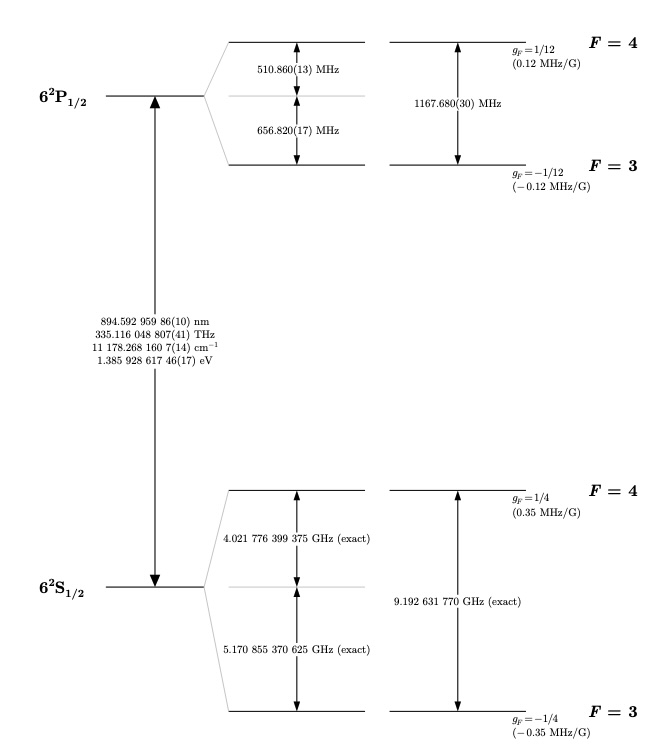
\includegraphics[width=\linewidth]{Figures/cs133_d1_hyperfine.jpeg}
        \par\smallskip
        \textbf{(a)} \({}^{133}\mathrm{Cs}\) D$_1$ line.
    \end{minipage}\hfill
    \begin{minipage}[t]{0.495\textwidth}
        \centering
        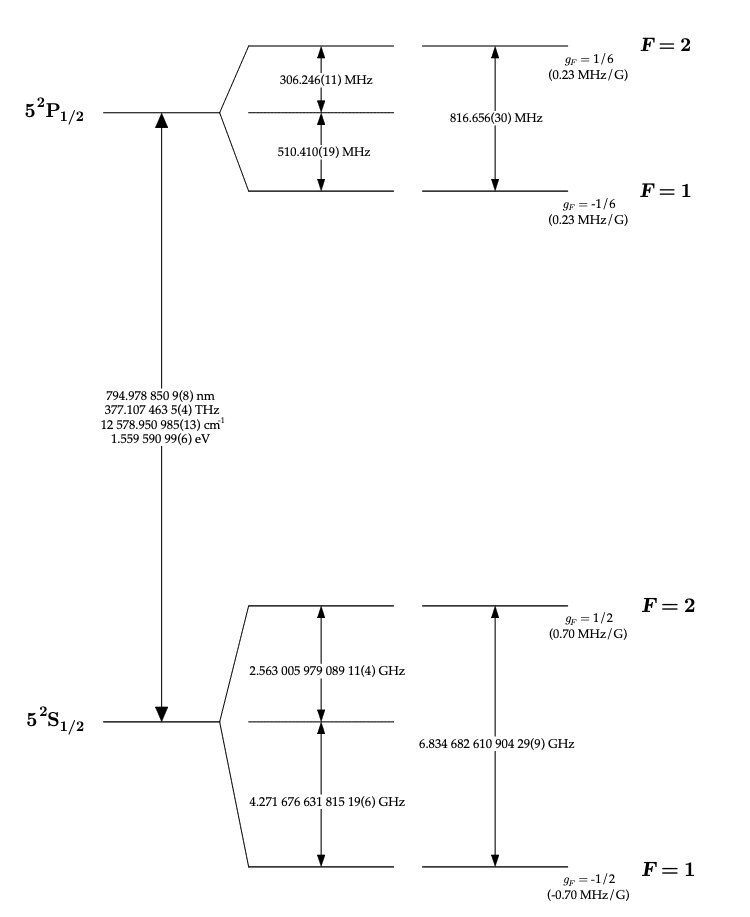
\includegraphics[width=\linewidth]{Figures/rb87_d1_hyperfine.jpeg}
        \par\smallskip
        \textbf{(b)} \({}^{87}\mathrm{Rb}\) D$_1$ line.
    \end{minipage}
    \caption[Hyperfine structure of the Cs and Rb D$_1$ lines.]{
        Hyperfine structure of the D$_1$ transitions used to construct alkali-metal
        \(\Lambda\)-type memories: \textbf{(a)} the
        \(6^2S_{1/2}\rightarrow6^2P_{1/2}\) transition of
        \({}^{133}\mathrm{Cs}\), reproduced from Ref.~\cite{CsDataLineSteck}, and
        \textbf{(b)} the \(5^2S_{1/2}\rightarrow5^2P_{1/2}\) transition of
        \({}^{87}\mathrm{Rb}\), reproduced from Ref.~\cite{RbDataLineSteck}.
        The diagrams show the ground- and excited-state hyperfine splittings and
        the approximate Land\'e factors. Splittings are drawn to scale within each
        hyperfine manifold, but the optical separation and the relative spacing
        of different manifolds are not shown on a common scale.
    }
    \label{fig:cs_rb_d1_hyperfine}
\end{figure}

%\section{Simulation Model}
\label{sec:simulation_model}

The  purpuse of the simulation model is to describe how a stored spin wave is converted into an optical field during retrieval and how this conversion is degraded when atoms move, acquire different phases, or leave the interaction region. The full Maxwell--Bloch writing dynamics are not solved. The stored ground-state coherence is used as the initial condition, and the retrieved field is calculated from the coherent radiation of the atoms that remain coupled to the retrievable collective mode.

Each atom contributing to readout is approximated as an ideal radiating dipole with a common internal orientation. Under this approximation, differences between atoms enter through their positions, phases, and weights, while the single-atom radiation pattern is treated as a common factor. Following the standard element-factor and array-factor decomposition used in antenna theory~\cite{AntenaCourseNotes}, the far-field amplitude in the observation direction $\hat{\mathbf n}$ may be written as
\begin{equation}
    \mathcal{E}_{\mathrm{out}}(\hat{\mathbf n},t)
    \propto
    \mathcal{E}_{\mathrm{dip}}(\hat{\mathbf n})
    \,
    \mathcal{A}(\hat{\mathbf n},t),
    \label{eq:field_element_array_factor}
\end{equation}
where $\mathcal{E}_{\mathrm{out}}(\hat{\mathbf n},t)$ is the emitted field amplitude, $\mathcal{E}_{\mathrm{dip}}(\hat{\mathbf n})$ is the single-dipole radiation factor, and $\mathcal{A}(\hat{\mathbf n},t)$ is the collective array factor. Since the relevant quantity is the relative retrieval into a selected optical mode, $\mathcal{E}_{\mathrm{dip}}(\hat{\mathbf n})$ is taken to be identical for all atoms and is not used to distinguish different trajectories.

The collective part of the field is represented by the weighted coherent sum
\begin{equation}
    \mathcal{A}(\hat{\mathbf n},t)
    =
    \sum_{j=1}^{N}
    W_j(t)
    \exp\left[
        i\Phi_j(\hat{\mathbf n},t)
    \right],
    \label{eq:array_factor_general}
\end{equation}
where $N$ is the number of simulated atoms, $W_j(t)$ is the complex amplitude weight assigned to atom $j$, and $\Phi_j(\hat{\mathbf n},t)$ is the phase with which that atom contributes to the field observed along $\hat{\mathbf n}$. The optical power associated with the selected direction is proportional to the squared modulus of the coherent amplitude,
\begin{equation}
    P(\hat{\mathbf n},t)
    \propto
    \left|
    \mathcal{A}(\hat{\mathbf n},t)
    \right|^2 .
    \label{eq:array_factor_power}
\end{equation}
Constructive collective emission is obtained when the phases in Eq.~\eqref{eq:array_factor_general} remain aligned. Random phases reduce the coherent sum even if individual atoms still radiate, because the field amplitudes no longer add efficiently before the modulus square is taken~\cite{AntenaCourseNotes,PsiL-odamIFm_GorshkovEtAl_2007}.

For spin-wave retrieval, the phase of each atomic contribution is set by the stored spin-wave grating, the read control field, the emitted optical mode, and any internal phase accumulated during storage. Using $\mathbf{k}_{\mathrm{out}}(\hat{\mathbf n})=k_{\mathrm{out}}\hat{\mathbf n}$, the phase is written as
\begin{equation}
    \Phi_j(\hat{\mathbf n},t)
    =
    \left(
        \Delta\mathbf{k}
        +
        \mathbf{k}_{\mathrm{c}}^{\mathrm{read}}
        -
        \mathbf{k}_{\mathrm{out}}(\hat{\mathbf n})
    \right)
    \cdot
    \mathbf{r}_j(t)
    -
    \phi_j(t),
    \label{eq:atom_retrieval_phase}
\end{equation}
where $\Delta\mathbf{k}$ is the spin-wave wave vector written during storage, $\mathbf{k}_{\mathrm{c}}^{\mathrm{read}}$ is the read-control wave vector, $\mathbf{k}_{\mathrm{out}}(\hat{\mathbf n})$ is the retrieved optical wave vector in the observation direction, $\mathbf{r}_j(t)$ is the position of atom $j$ after storage time $t$, and $\phi_j(t)$ is the additional phase accumulated by the ground-state coherence. Constructive retrieval is obtained when the position-dependent phase in Eq.~\eqref{eq:atom_retrieval_phase} is stationary across the ensemble. Following the usual spin-wave phase-matching condition~\cite{PsiL-odamIFm_GorshkovEtAl_2007}, this gives
\begin{equation}
    \mathbf{k}_{\mathrm{out}}
    =
    \Delta\mathbf{k}
    +
    \mathbf{k}_{\mathrm{c}}^{\mathrm{read}}.
    \label{eq:simulation_phase_matching}
\end{equation}
The preferred retrieval direction is therefore fixed by the spatial phase stored in the atomic coherence and by the geometry of the read control field.

The weights $W_j(t)$ describe the amplitude with which each atom contributes to the selected mode. Uniform weights would be obtained for an ideal ensemble illuminated homogeneously by the relevant optical fields. In a finite memory system with nonuniform optical mode profiles, atoms near the centre of the signal and control beams couple more strongly than atoms in the wings. The stored spin wave therefore carries an amplitude envelope, and the coherent sum in Eq.~\eqref{eq:array_factor_general} must be evaluated as a weighted sum.

For a Gaussian optical mode, the transverse field envelope is taken as
\begin{equation}
    u_{\ell}(\mathbf{r})
    =
    \exp\left[
        -\frac{\rho_{\ell}^2(\mathbf{r})}{w_{\ell}^2}
    \right],
    \label{eq:gaussian_field_envelope}
\end{equation}
where the subscript $\ell$ labels the optical field, $\rho_{\ell}(\mathbf{r})$ is the transverse distance from the propagation axis of that field, and $w_{\ell}$ is the Gaussian field radius. The corresponding intensity profile is
\begin{equation}
    I_{\ell}(\mathbf{r})
    \propto
    \left|
    u_{\ell}(\mathbf{r})
    \right|^2
    =
    \exp\left[
        -\frac{2\rho_{\ell}^2(\mathbf{r})}{w_{\ell}^2}
    \right].
    \label{eq:gaussian_intensity_profile}
\end{equation}
If the beam diameter is specified by the full width at half maximum of the intensity, the field radius in Eq.~\eqref{eq:gaussian_field_envelope} is related to $\mathrm{FWHM}_{\ell}$ by
\begin{equation}
    \mathrm{FWHM}_{\ell}
    =
    w_{\ell}\sqrt{2\ln 2}.
    \label{eq:fwhm_to_waist}
\end{equation}

The initial spin-wave profile is determined by the overlap of the signal and write-control fields. Following the spin-wave description of ensemble memories~\cite{PsiL-odamIFm_GorshkovEtAl_2007}, the stored coherence may be written as
\begin{equation}
    S(\mathbf{r},0)
    =
    \mathcal{N}
    \,
    u_{\mathrm{sig}}(\mathbf{r})
    u_{\mathrm{c}}^{*}(\mathbf{r})
    \exp\left[
        i
        \left(
            \mathbf{k}_{\mathrm{sig}}^{\mathrm{write}}
            -
            \mathbf{k}_{\mathrm{c}}^{\mathrm{write}}
        \right)
        \cdot
        \mathbf{r}
    \right],
    \label{eq:initial_spin_wave_profile}
\end{equation}
where $S(\mathbf{r},0)$ is the initial ground-state coherence, $\mathcal{N}$ is a normalization constant, $u_{\mathrm{sig}}(\mathbf{r})$ is the signal-mode envelope, $u_{\mathrm{c}}(\mathbf{r})$ is the write-control envelope, $\mathbf{k}_{\mathrm{sig}}^{\mathrm{write}}$ is the signal wave vector, and $\mathbf{k}_{\mathrm{c}}^{\mathrm{write}}$ is the write-control wave vector. The conjugation of $u_{\mathrm{c}}(\mathbf{r})$ reflects that the stored coherence is written by the signal field relative to the control field.

In the particle representation, the continuous spin wave is sampled by atoms at positions $\mathbf{r}_j(0)$. The initial amplitude weight is
\begin{equation}
    W_j(0)
    =
    \mathcal{N}
    \,
    u_{\mathrm{sig}}\!\left(\mathbf{r}_j(0)\right)
    u_{\mathrm{c}}^{*}\!\left(\mathbf{r}_j(0)\right),
    \label{eq:initial_atomic_weight}
\end{equation}
where $W_j(0)$ is the initial contribution of atom $j$ to the stored mode. The spin-wave phase is kept outside the weight and is included explicitly in Eq.~\eqref{eq:atom_retrieval_phase}. This separation assigns the mode amplitude to $W_j(t)$ and the retrieval interference to $\Phi_j(\hat{\mathbf n},t)$.

Atomic motion is included by evolving the positions $\mathbf{r}_j(t)$ during storage. In a warm vapour, atoms move through the optical mode, collide with buffer-gas atoms, and may encounter the cell walls. Even when the internal coherence survives, the atom contributes from a different position at readout. Since the phase in Eq.~\eqref{eq:atom_retrieval_phase} is evaluated at $\mathbf{r}_j(t)$, motion changes the collective interference pattern and can reduce the phase-matched retrieved field.

For diffusive motion, the stochastic displacement during a time step $\Delta t$ is sampled as~\cite{MonteCarloNotes}
\begin{equation}
    \mathbf{r}_j(t+\Delta t)
    =
    \mathbf{r}_j(t)
    +
    \sqrt{2D\Delta t}\,
    \boldsymbol{\xi}_j,
    \label{eq:diffusive_position_update}
\end{equation}
where $D$ is the diffusion coefficient and $\boldsymbol{\xi}_j$ is a three-dimensional random vector with independent normally distributed components of zero mean and unit variance. This update gives the three-dimensional diffusion result~\cite{MonteCarloNotes}
\begin{equation}
    \left\langle
    \left|
    \mathbf{r}_j(t+\Delta t)-\mathbf{r}_j(t)
    \right|^2
    \right\rangle
    =
    6D\Delta t,
    \label{eq:diffusion_msd}
\end{equation}
where the angle brackets denote an average over trajectories. Other transport models can be incorporated by replacing the update rule for $\mathbf{r}_j(t)$.

A position-dependent ground-state splitting produces an additional phase. The spatially uniform part of the splitting produces only a common phase and is removed from the retrieval amplitude. The relevant contribution is the differential shift $\Delta\omega_{sg}(\mathbf{r})$, which gives
\begin{equation}
    \phi_j(t)
    =
    \int_0^t
    \Delta\omega_{sg}\!\left(\mathbf{r}_j(t')\right)
    \,dt',
    \label{eq:internal_phase_integral}
\end{equation}
where $t'$ is the integration variable. A homogeneous shift gives the same $\phi_j(t)$ for every atom and leaves the collective interference unchanged. Spatially varying shifts give trajectory-dependent phases and reduce the phase-matched spin-wave component.

Wall relaxation and other loss mechanisms are included through a survival factor. The time-dependent atomic weight is written as
\begin{equation}
    W_j(t)
    =
    W_j(0)
    \,
    \eta_j(t)
    \,
    u_{\mathrm{read}}\!\left(\mathbf{r}_j(t)\right),
    \label{eq:time_dependent_weight}
\end{equation}

where $\eta_j(t)$ is the survival factor of the ground-state coherence of atom $j$, and $u_{\mathrm{read}}(\mathbf{r}_j(t))$ is the spatial envelope associated with the readout mode at the atom position. Ideal coherent motion is recovered by setting $\eta_j(t)=1$. Depolarizing events reduce $\eta_j(t)$ and therefore remove part of the atomic contribution from the coherent sum.

Wall-induced relaxation is represented phenomenologically through the mean number of wall collisions that an atom can undergo before losing its ground-state coherence. This parameter, denoted by $N_{\mathrm{b}}$, does not describe the microscopic atom--surface interaction of a specific coating. It provides an effective way to compare uncoated cells with anti-relaxation coatings by changing the probability that coherence survives repeated wall encounters. If atom $j$ has experienced $n_j(t)$ wall collisions by time $t$, the survival factor is taken to be
\begin{equation}
    \eta_j(t)
    =
    \left(
        1-\frac{1}{N_{\mathrm{b}}}
    \right)^{n_j(t)}.
    \label{eq:wall_survival_factor}
\end{equation}
This expression assigns the same survival probability to each wall collision and assumes independent relaxation events. The physical interpretation of $N_{\mathrm{b}}$ and its relation to coated warm-vapour cells will be discuss in section~\ref{sec:coatings}

The simulated retrieval amplitude in a target direction $\hat{\mathbf n}_{\mathrm{tar}}$ is then
\begin{equation}
    \mathcal{A}_{\mathrm{tar}}(t)
    =
    \sum_{j=1}^{N}
    W_j(t)
    \exp\left[
        i\Phi_j(\hat{\mathbf n}_{\mathrm{tar}},t)
    \right],
    \label{eq:target_mode_amplitude}
\end{equation}
where $\mathcal{A}_{\mathrm{tar}}(t)$ is the complex field amplitude emitted into the target optical direction. The corresponding target-mode power is
\begin{equation}
    P_{\mathrm{tar}}(t)
    \propto
    \left|
    \mathcal{A}_{\mathrm{tar}}(t)
    \right|^2 .
    \label{eq:target_mode_power}
\end{equation}

As the detected mode is a fibre mode rather than a single far-field direction, the retrieved amplitude is projected onto the angular fibre mode. The fibre-coupled amplitude is
\begin{equation}
    \mathcal{A}_{\mathrm{fib}}(t)
    =
    \int d\Omega\,
    u_{\mathrm{fib}}^{*}(\hat{\mathbf n})
    \mathcal{E}_{\mathrm{out}}(\hat{\mathbf n},t),
    \label{eq:fibre_overlap_integral}
\end{equation}
where $u_{\mathrm{fib}}(\hat{\mathbf n})$ is the normalized angular mode of the fibre and $d\Omega$ is the differential solid angle. The fibre-coupled power is
\begin{equation}
    P_{\mathrm{fib}}(t)
    \propto
    \left|
    \mathcal{A}_{\mathrm{fib}}(t)
    \right|^2 .
    \label{eq:fibre_power}
\end{equation}
The useful retrieved signal is therefore determined by a coherent mode overlap, rather than by the total optical power emitted into all directions.

The Monte Carlo calculation evaluates the coherent sums by sampling atoms and trajectories. Each sampled atom is assigned an initial position, an optical weight, a stochastic trajectory, a survival factor, and an accumulated internal phase. At each timestep, the retrieval amplitude is evaluated from the current positions, phases, and weights. The numerical result therefore estimates an ensemble average over possible atomic configurations and histories~\cite{MonteCarloNotes}.

For the target direction, the Monte Carlo estimator of the amplitude is
\begin{equation}
    \widehat{\mathcal{A}}_{\mathrm{tar}}(t)
    =
    \frac{1}{N_{\mathrm{MC}}}
    \sum_{j=1}^{N_{\mathrm{MC}}}
    W_j(t)
    \exp\left[
        i\Phi_j(\hat{\mathbf n}_{\mathrm{tar}},t)
    \right],
    \label{eq:monte_carlo_amplitude_estimator}
\end{equation}
where $N_{\mathrm{MC}}$ is the number of Monte Carlo samples and the hat denotes a numerical estimator. The associated power estimator is
\begin{equation}
    \widehat{P}_{\mathrm{tar}}(t)
    \propto
    \left|
    \widehat{\mathcal{A}}_{\mathrm{tar}}(t)
    \right|^2 .
    \label{eq:monte_carlo_power_estimator}
\end{equation}
Under independent sampling, the statistical error of the amplitude estimator scales as $N_{\mathrm{MC}}^{-1/2}$~\cite{MonteCarloNotes}.

The normalized retrieval observable is defined as
\begin{equation}
    \mathcal{R}_{\mathrm{fib}}(t)
    =
    \frac{P_{\mathrm{fib}}(t)}
    {P_{\mathrm{tot}}(0)},
    \label{eq:normalized_fibre_retrieval}
\end{equation}
where $P_{\mathrm{fib}}(t)$ is the fibre-coupled retrieved power after storage time $t$, and $P_{\mathrm{tot}}(0)$ is the total emitted power at zero storage time. This normalization removes the arbitrary absolute scale of the emitted field while retaining the decay of the retrievable mode. The observable is therefore sensitive to phase mismatch, loss of beam overlap, and survival of the ground-state coherence.

\section{Introduction to the Chapter}
\label{sec:chapter_intro}

This chapter presents the numerical results obtained with the \texttt{radpattern} simulation framework. The chapter is organized from a macroscopic warm-vapour reference geometry to a compact boundary-dominated cell, and finally to the contactless ultracold regime.

The main observable used throughout the chapter is the normalized retrievable-mode coupling,
\begin{equation}
    \eta(t)
    =
    \frac{P_{\mathrm{fib}}(t)}{P_{\mathrm{tot}}(0)} ,
    \label{eq:eta_pfibt_ptot0}
\end{equation}
where $P_{\mathrm{fib}}(t)$ is the power coupled into the target fibre mode at time $t$, and $P_{\mathrm{tot}}(0)$ is the initial total emitted power.

The coherent fibre-coupled amplitude is evaluated from the ensemble as
\begin{equation}
    A_{\mathrm{fib}}(t)
    \propto
    \sum_{j}
    w_j(t)
    e^{i\phi_j(t)}
    u_{\mathrm{fib}}^*\!\left(\mathbf r_j(t)\right),
    \label{eq:fiber_mode_sum}
\end{equation}
where $w_j(t)$ is the atomic weight, $\phi_j(t)$ is the accumulated spin-wave phase, $u_{\mathrm{fib}}$ is the target optical mode, and $\mathbf r_j(t)$ is the position of atom $j$.

\begin{figure}[htbp]
    \centering
    \includegraphics[width=0.85\textwidth]{Figures/spinwave_retrieval_concept.jpeg}
    \caption{Temporary caption: Schematic of the stored spin wave and the retrieved fibre-coupled mode. The figure should define the signal beam, control beam, ensemble, spin-wave phase, and target output mode.}
    \label{fig:chapter_concept_spinwave_retrieval}
\end{figure}

\section{Macroscopic Validation and Sensitivity Checks}
\label{sec:macroscopic_validation}

This section uses a ${}^{133}\mathrm{Cs}$ warm-vapour reference geometry based on a long cylindrical cell. The baseline geometry is a $\SI{75}{\milli\metre}$ long and $\SI{4}{\milli\metre}$ diameter cell operated near $\SI{75}{\celsius}$, with $N_2$ buffer gas and focused signal and control beams.

\begin{figure}[htbp]
    \centering
    \includegraphics[width=0.85\textwidth]{Figures/jutisz_reference_geometry.jpeg}
    \caption{Temporary caption: Reference warm-vapour geometry used for validation. The figure should show the $\SI{75}{\milli\metre}$ by $\SI{4}{\milli\metre}$ cylindrical cell, the signal and control beams, the buffer gas, and the fibre-coupled output mode.}
    \label{fig:jutisz_reference_geometry}
\end{figure}

\subsection{Directional Emission and Coherent Radiative Profiles}
\label{subsec:directional_emission}

The first validation step is to verify that the stored spin wave produces directional collective emission. The simulation treats the ensemble as a set of phased microscopic emitters, whose far-field interference determines the retrieved optical mode.

\begin{figure}[htbp]
    \centering
    \begin{minipage}[t]{0.48\textwidth}
        \centering
        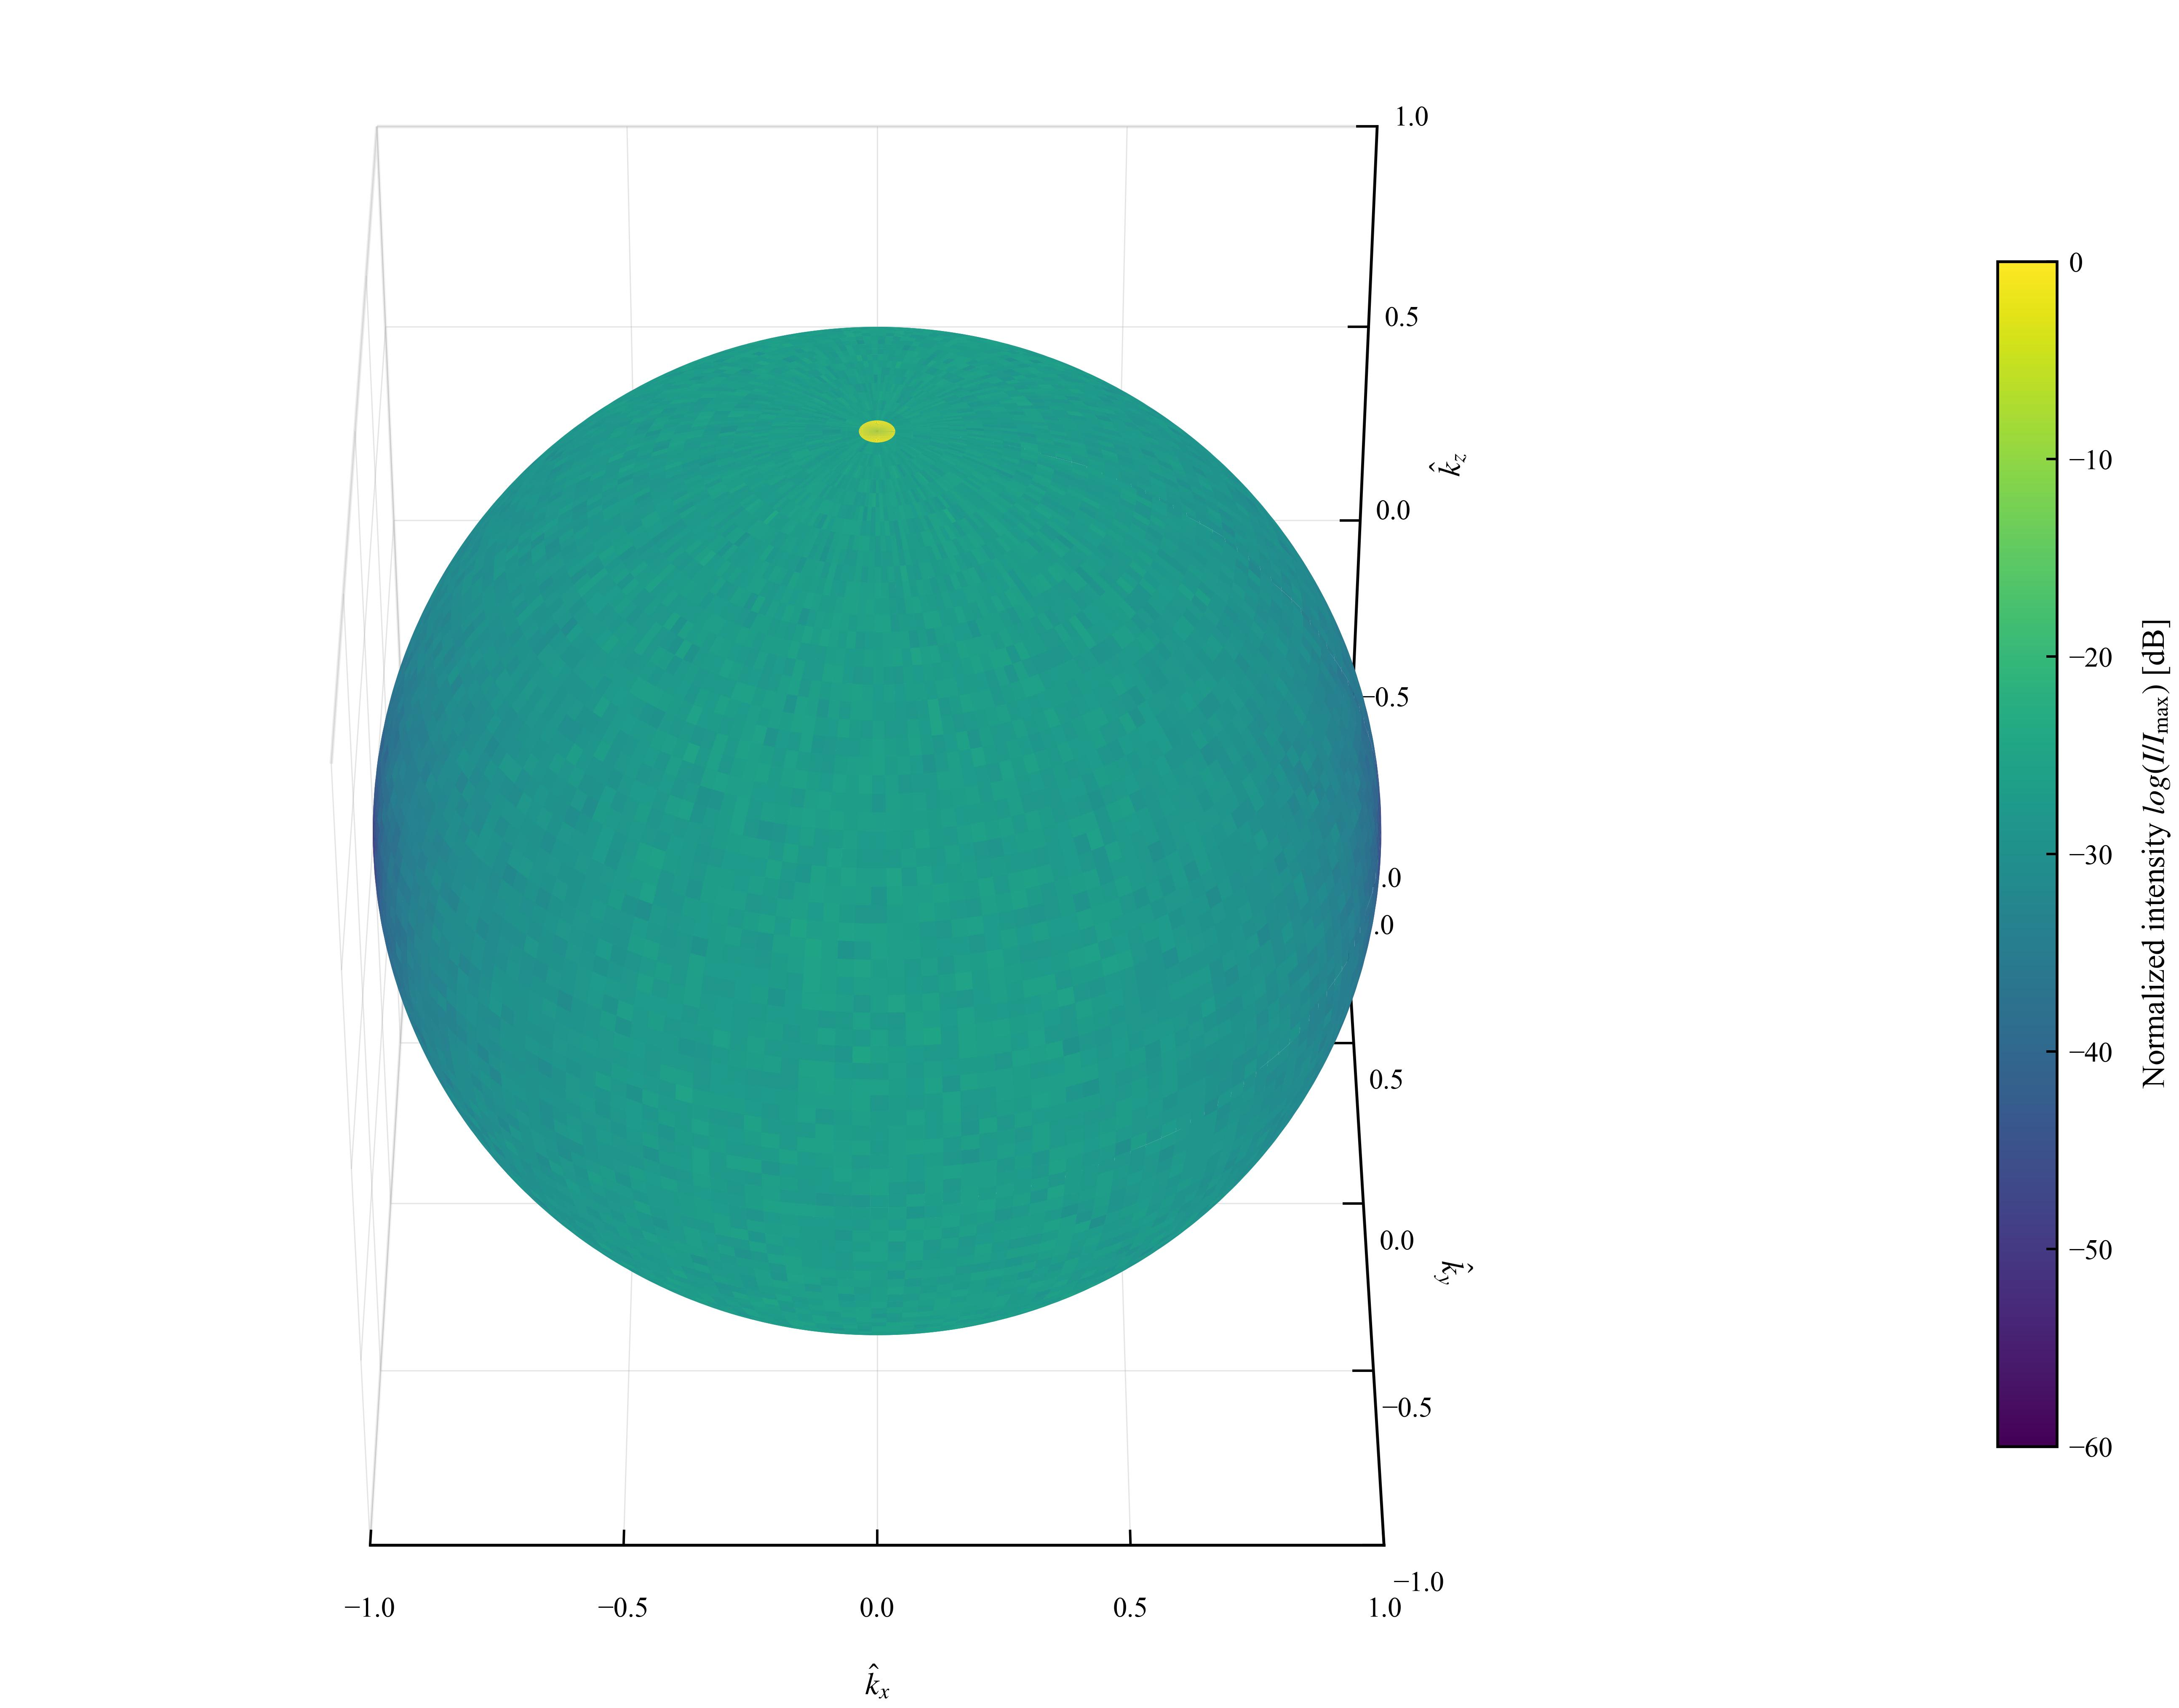
\includegraphics[width=\textwidth]{Figures/far_field_angular_emission_profile.jpeg}
    \end{minipage}
    \hfill
    \begin{minipage}[t]{0.48\textwidth}
        \centering
        \includegraphics[width=\textwidth]{Figures/weighted_atom_cloud_distribution.jpeg}
    \end{minipage}
    \caption{Temporary caption: Left: far-field angular emission profile from the collective spin-wave distribution. Right: three-dimensional atom cloud with normalized atomic weights $|w|_{\mathrm{norm}}$. Together, these plots show that the retrieved signal is a directional coherent-emission mode rather than an incoherent atom-number signal.}
    \label{fig:directional_emission_cloud_weights}
\end{figure}

\subsection{Convergence and Statistical Stability}
\label{subsec:mc_convergence}

Monte Carlo convergence is checked by comparing individual stochastic realizations with the ensemble-averaged coupling curve. This verifies that the simulated decay is not dominated by sampling noise or by a small number of rare trajectories.

\begin{figure}[htbp]
    \centering
    \includegraphics[width=0.78\textwidth]{Figures/mc_convergence_realizations.jpeg}
    \caption{Temporary caption: Monte Carlo convergence check. Thin curves show individual realizations, while the thick curve shows the ensemble average. The figure should demonstrate that the long-time decay and plateau features are statistically stable.}
    \label{fig:mc_convergence}
\end{figure}

\subsection{Gas-Phase Transport and Spatial Escape}
\label{subsec:pressure_scans}

The buffer gas pressure controls the diffusion coefficient and therefore the time scale over which atoms leave the high-overlap optical mode. Pressure scans are used to validate the gas-phase transport model.

\begin{figure}[htbp]
    \centering
    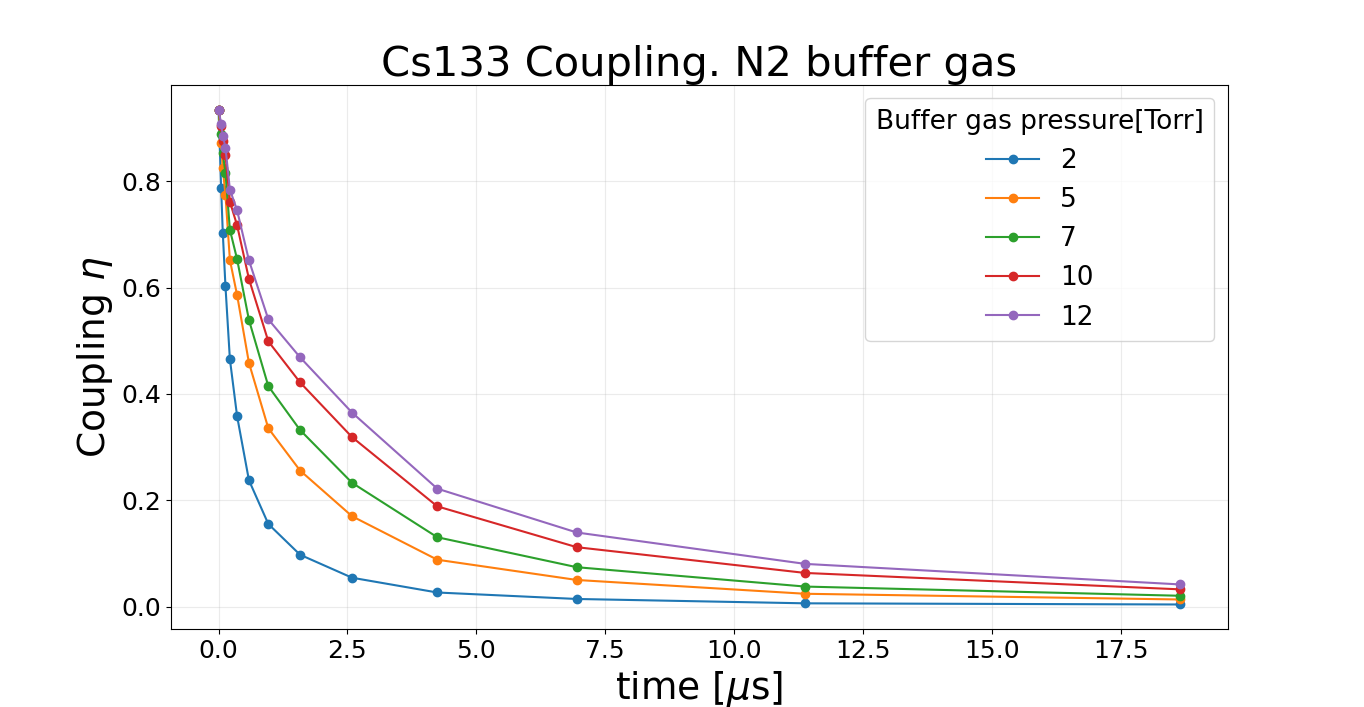
\includegraphics[width=0.78\textwidth]{Figures/pressure_scan_coupling_decay.jpeg}
    \caption{Temporary caption: Coupling decay $\eta(t)$ for different $N_2$ buffer gas pressures in the $\SI{75}{\milli\metre}$ reference cell. Higher pressure reduces diffusion and slows the loss of fibre-mode overlap.}
    \label{fig:pressure_scan_eta}
\end{figure}

\begin{figure}[htbp]
    \centering
    \includegraphics[width=0.72\textwidth]{Figures/pressure_scan_decay_time.jpeg}
    \caption{Temporary caption: Extracted characteristic decay time $\tau_{\eta}$ as a function of $N_2$ buffer gas pressure. This plot summarizes the pressure dependence of the retrievable-mode lifetime.}
    \label{fig:pressure_scan_tau}
\end{figure}

\subsection{Beam-Size Dependence}
\label{subsec:beam_size_dependence}

The optical beam dimensions set the spatial region over which atoms contribute efficiently to the retrieved mode. Larger beams are expected to reduce diffusion-driven escape from the optical mode, while smaller beams increase sensitivity to atomic motion.

\begin{figure}[htbp]
    \centering
    \includegraphics[width=0.78\textwidth]{Figures/beam_size_coupling_decay.jpeg}
    \caption{Temporary caption: Coupling decay $\eta(t)$ for different signal or control beam diameters. Larger beams produce slower mode-overlap decay because atoms remain inside the optically weighted region for longer times.}
    \label{fig:beam_size_eta}
\end{figure}

\begin{figure}[htbp]
    \centering
    \includegraphics[width=0.72\textwidth]{Figures/beam_size_decay_time.jpeg}
    \caption{Temporary caption: Extracted decay time $\tau_{\eta}$ as a function of beam diameter. This plot summarizes the sensitivity of the retrievable-mode lifetime to the transverse optical mode size.}
    \label{fig:beam_size_tau}
\end{figure}

\section{Phase-Gradient and Vector Perturbations in Bulk Media}
\label{sec:phase_gradient_perturbations}

This section isolates mechanisms that degrade the coherent sum without requiring atoms to collide with a physical boundary. The two main perturbations are geometric phase mismatch from beam misalignment and Zeeman dephasing from magnetic-field gradients.

\subsection{Geometric Phase Mismatch from Control-Beam Angle}
\label{subsec:control_beam_angle}

A change in the control-beam direction changes the phase-matching condition. The relevant wave-vector mismatch is
\begin{equation}
    \Delta \mathbf{k}
    =
    \mathbf{k}_{\mathrm{sig}}
    -
    \mathbf{k}_{\mathrm{c}} .
    \label{eq:delta_k_angle}
\end{equation}
Small milliradian angular offsets impose a transverse phase gradient across the ensemble and reduce the constructive interference into the target mode.

\begin{figure}[htbp]
    \centering
    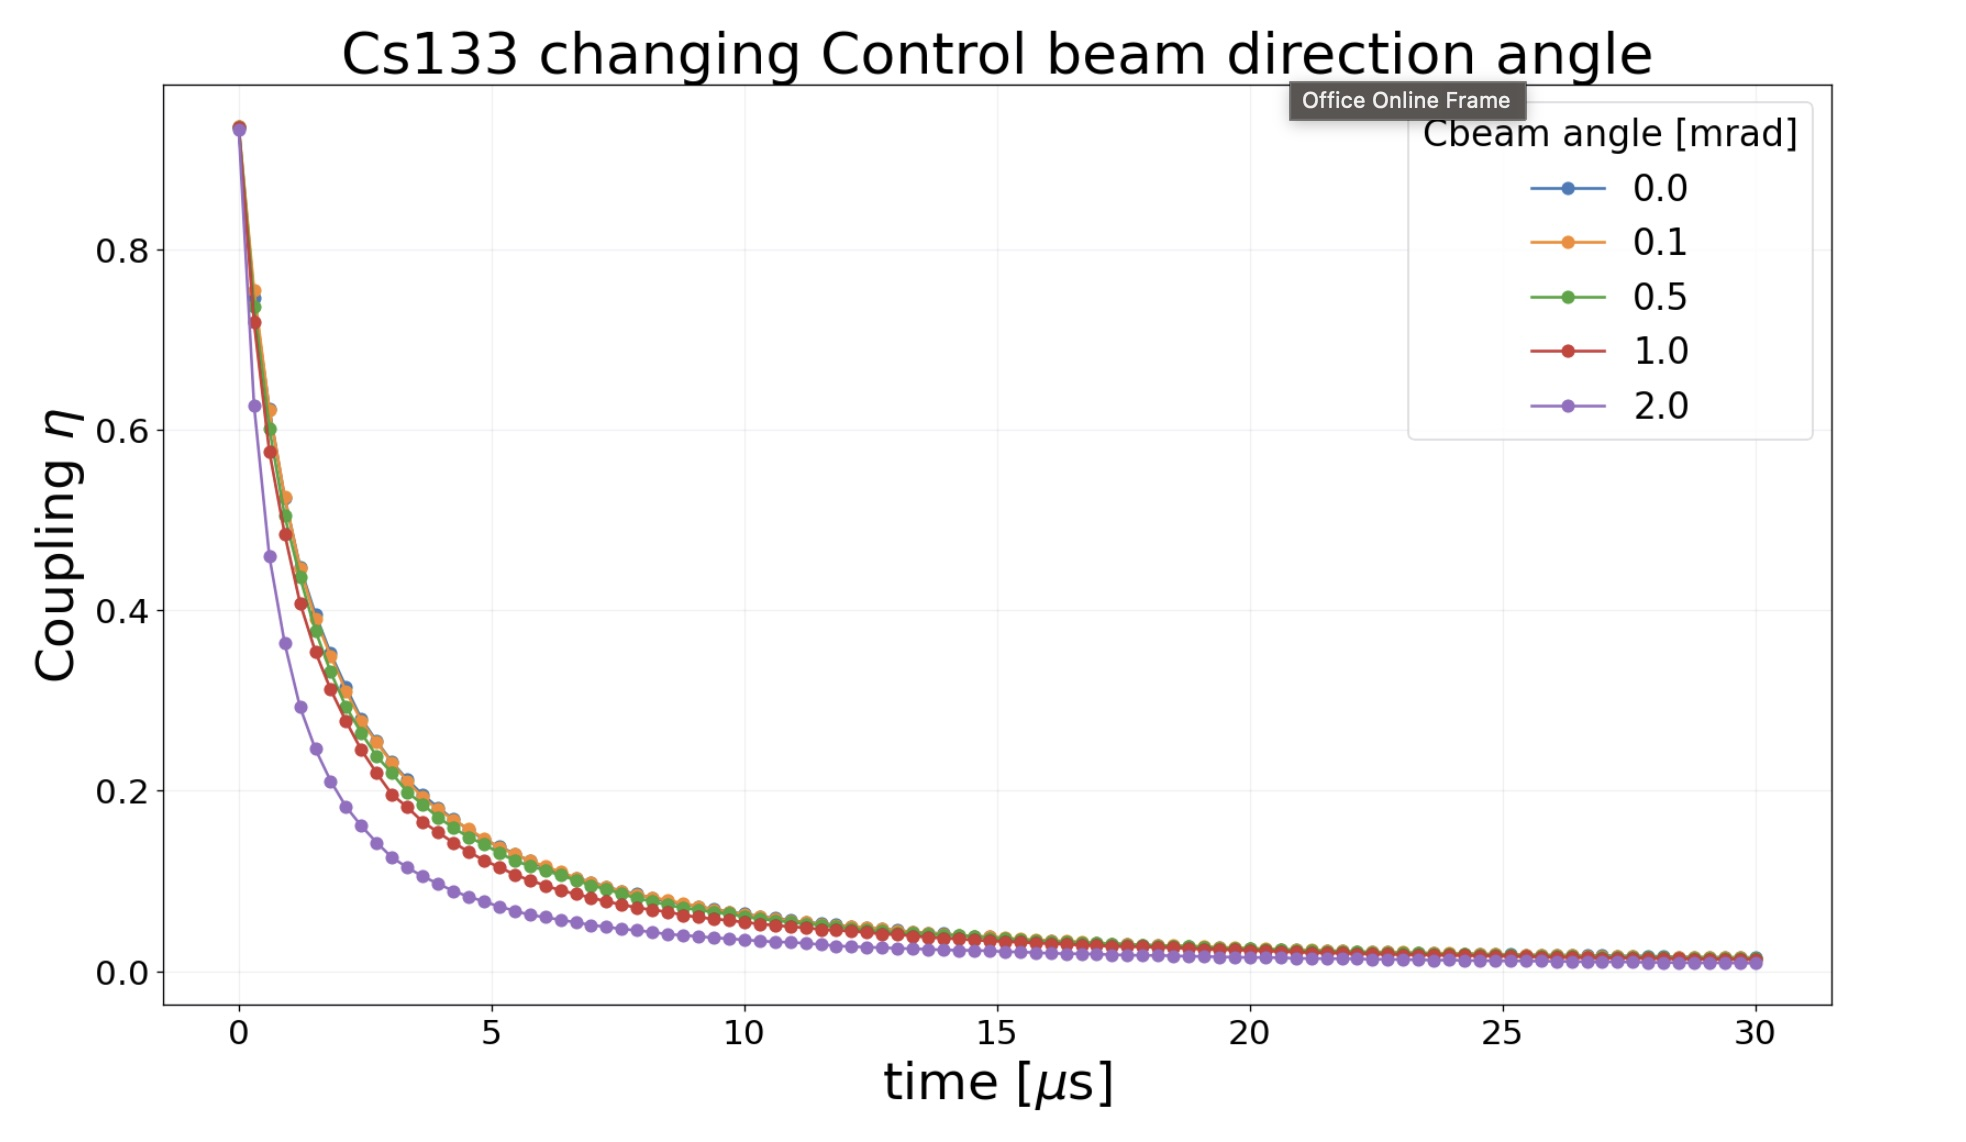
\includegraphics[width=0.78\textwidth]{Figures/control_beam_angle_scan.jpeg}
    \caption{Temporary caption: Coupling decay $\eta(t)$ for different control-beam angular offsets. The scan should include milliradian-scale angles and show the degradation of phase-matched retrieval with increasing angular mismatch.}
    \label{fig:control_angle_scan}
\end{figure}

\begin{figure}[htbp]
    \centering
    \includegraphics[width=0.72\textwidth]{Figures/control_beam_angle_tolerance_summary.jpeg}
    \caption{Temporary caption: Coupling at a fixed storage time, or fitted decay time $\tau_{\eta}$, as a function of control-beam angle. This plot summarizes the angular tolerance of the retrieval geometry.}
    \label{fig:control_angle_summary}
\end{figure}

\subsection{Zeeman Scrambling from Magnetic-Field Gradients}
\label{subsec:magnetic_gradient}

A uniform magnetic field produces only a global phase. By contrast, a magnetic-field gradient produces position-dependent spin-wave precession,
\begin{equation}
    \phi_j(t)
    =
    \phi_j(0)
    -
    \omega_{sg}\!\left(\mathbf r_j\right)t ,
    \label{eq:position_dependent_phase}
\end{equation}
which reduces the coherent fibre-coupled amplitude.

\begin{figure}[htbp]
    \centering
    \begin{minipage}[t]{0.48\textwidth}
        \centering
        \includegraphics[width=\textwidth]{Figures/cs_magnetic_gradient_scan.jpeg}
    \end{minipage}
    \hfill
    \begin{minipage}[t]{0.48\textwidth}
        \centering
        \includegraphics[width=\textwidth]{Figures/rb_magnetic_gradient_scan.jpeg}
    \end{minipage}
    \caption{Temporary caption: Magnetic-field-gradient scans for Cs and Rb configurations. The curves show how spatially varying Zeeman shifts dephase the spin wave and reduce the phase-matched fibre coupling.}
    \label{fig:magnetic_gradient_cs_rb}
\end{figure}

\section{The Compact-Cell Boundary Regime}
\label{sec:compact_cell_boundary_regime}

The validated model is next applied to a compact ${}^{133}\mathrm{Cs}$ cell with diameter $\SI{1}{\milli\metre}$ and length $\SI{1}{\centi\metre}$. The control beam has diameter $\SI{0.8}{\milli\metre}$, and the signal beam has diameter $\SI{0.3}{\milli\metre}$. In this geometry, the control beam occupies a large fraction of the available transverse cell size, so wall interactions and boundary reflections can no longer be treated as negligible.

\begin{figure}[htbp]
    \centering
    \includegraphics[width=0.78\textwidth]{Figures/compact_cell_geometry.jpeg}
    \caption{Temporary caption: Compact-cell geometry. The figure should show the $\SI{1}{\milli\metre}$ diameter cell, the $\SI{1}{\centi\metre}$ length, the $\SI{0.8}{\milli\metre}$ control beam, the $\SI{0.3}{\milli\metre}$ signal beam, and the proximity of the optical modes to the walls.}
    \label{fig:compact_cell_geometry}
\end{figure}

\subsection{Breakdown of a Single-Exponential Lifetime}
\label{subsec:single_exponential_breakdown}

In the compact geometry, the coupling decay can contain a fast initial loss followed by a slow tail or plateau. This occurs because atoms can reflect from the boundaries and re-enter the high-overlap region. Therefore, a single exponential form,
\begin{equation}
    \eta(t)
    =
    \eta_0 e^{-t/\tau},
    \label{eq:single_exp_fit}
\end{equation}
may not be a physically complete description of the compact-cell dynamics.

\begin{figure}[htbp]
    \centering
    \includegraphics[width=0.78\textwidth]{Figures/compact_cell_long_time_decay.jpeg}
    \caption{Temporary caption: Long-time coupling decay in the compact $\SI{1}{\milli\metre}$ cell. The plot should highlight the non-single-exponential structure, including the initial decay, slow tail, and possible plateau produced by reflection and re-entry.}
    \label{fig:compact_cell_long_time_decay}
\end{figure}

\subsection{Surface Chemistry Abstraction: Coating and Wall-Bounce Scans}
\label{subsec:coating_wall_bounce_scans}

Wall depolarization is represented by an effective survival parameter $N_{\text{b}}$, defined as the average number of wall collisions an atom can undergo before losing its spin-wave coherence. The scan covers poor wall survival up to nearly ideal anti-relaxation behaviour, for example once $N_{\text{b}}\sim \num{1e3}\text{ to }\num{1e4}$ and above.

\begin{figure}[htbp]
    \centering
    \includegraphics[width=0.78\textwidth]{Figures/compact_cell_wall_survival_decay.jpeg}
    \caption{Temporary caption: Compact-cell coupling decay $\eta(t)$ for different wall-survival parameters $N_{\text{b}}$. The scan should include values from $N_{\text{b}}=\num{1e3}$ to $N_{\text{b}}=\num{1e12}$, showing the transition from wall-limited decay to a geometry- or diffusion-limited plateau.}
    \label{fig:compact_cell_nbounces_eta}
\end{figure}

\begin{figure}[htbp]
    \centering
    \includegraphics[width=0.72\textwidth]{Figures/compact_cell_wall_survival_design.jpeg}
    \caption{Temporary caption: Design summary plot showing $\eta(t_{\mathrm{target}})$ or $\tau_{\eta}$ as a function of $N_{\text{b}}$. The expected behaviour is a strong improvement at low $N_{\text{b}}$, followed by saturation once wall relaxation is no longer the dominant limitation.}
    \label{fig:compact_cell_nbounces_design}
\end{figure}

\subsection{Beam Size, Coating Quality, and Buffer Gas Coupling}
\label{subsec:beam_coating_pressure_tradeoff}

The compact geometry couples several design parameters. Increasing the beam size improves mode-overlap lifetime but also brings the optical mode closer to the walls. Increasing buffer gas pressure slows diffusion, while improving the coating increases survival during wall encounters. These variables should therefore be interpreted together.

\begin{figure}[htbp]
    \centering
    \includegraphics[width=0.78\textwidth]{Figures/compact_cell_joint_design_map.jpeg}
    \caption{Temporary caption: Joint design map for the compact cell. Possible axes include beam diameter and $N_{\text{b}}$, or buffer gas pressure and $N_{\text{b}}$, with colour representing $\eta(t_{\mathrm{target}})$ or $\tau_{\eta}$.}
    \label{fig:compact_cell_design_map}
\end{figure}

\section{Contactless Confinement: The Ultracold BEC Regime}
\label{sec:bec_regime}

The ultracold regime provides an alternative limit in which physical wall collisions are removed. Instead of wall-limited diffusion, the relevant spatial evolution comes from the initial trapped density distribution, ballistic expansion, gravitational sag, and trap-induced motion.

\subsection{Mapping the Trap Profile}
\label{subsec:bec_trap_profile}

The initial density distribution is no longer uniform inside a cylinder. Instead, the atom cloud follows a trapped density profile, such as a Gaussian or Thomas-Fermi distribution. This modifies the initial spatial overlap with the optical mode.

\begin{figure}[htbp]
    \centering
    \begin{minipage}[t]{0.48\textwidth}
        \centering
        \includegraphics[width=\textwidth]{Figures/bec_density_distribution.jpeg}
    \end{minipage}
    \hfill
    \begin{minipage}[t]{0.48\textwidth}
        \centering
        \includegraphics[width=\textwidth]{Figures/bec_weight_distribution.jpeg}
    \end{minipage}
    \caption{Temporary caption: Ultracold cloud initialization. Left: three-dimensional density distribution of the trapped cloud. Right: spatial distribution of the normalized atomic weights $|w|_{\mathrm{norm}}$ relative to the target optical mode.}
    \label{fig:bec_density_weights}
\end{figure}

\subsection{Free Expansion and Trap-Induced Drift}
\label{subsec:bec_motion_profiles}

If the trap is released, the cloud expands ballistically. The characteristic thermal velocity $v_{\text{th}}$ produces a time-dependent spatial footprint, which modifies the spin-wave overlap with the fibre mode. If the trap remains on, the dominant motion may instead come from residual drift, gravitational sag, or trap oscillations.

\begin{figure}[htbp]
    \centering
    \includegraphics[width=0.78\textwidth]{Figures/bec_motion_decay.jpeg}
    \caption{Temporary caption: Coupling decay $\eta(t)$ for different ultracold motion models, such as released ballistic expansion and trapped-cloud drift. The comparison isolates spatial overlap loss without wall collisions.}
    \label{fig:bec_motion_eta}
\end{figure}

\section{Engineering Synthesis: Comparing the Two Extremes}
\label{sec:engineering_synthesis}

The warm compact cell and ultracold cloud represent two limiting regimes of spatial-mode degradation. The compact warm cell is boundary dominated, while the ultracold cloud is contactless but sensitive to expansion and drift.

\subsection{Collision-Dominated and Ballistic Regimes}
\label{subsec:collision_vs_ballistic}

The decay profiles from both regimes can be compared directly. A compact coated cell can show non-single-exponential decay and long-time plateaus due to reflection and re-entry. An ultracold released cloud is expected to show smoother overlap loss associated with ballistic expansion or drift.

\begin{figure}[htbp]
    \centering
    \includegraphics[width=0.78\textwidth]{Figures/warm_compact_vs_bec_decay.jpeg}
    \caption{Temporary caption: Direct comparison of representative coupling decays from the compact warm-vapour cell and the ultracold cloud. The figure should emphasize the difference between boundary-mediated re-entry and smooth ballistic or trap-induced spatial loss.}
    \label{fig:warm_compact_vs_bec_decay}
\end{figure}

\subsection{Pressure, Coating, Temperature, and Trap Parameters}
\label{subsec:parameter_synthesis}

The final comparison summarizes the controlling design parameters in each regime. Warm-vapour operation depends on buffer gas pressure, temperature, beam size, and wall-survival parameter $N_{\text{b}}$. Ultracold operation depends on trap frequencies, release time, temperature, cloud size, and spatial drift.

\begin{figure}[htbp]
    \centering
    \includegraphics[width=0.82\textwidth]{Figures/warm_vapor_bec_parameter_synthesis.jpeg}
    \caption{Temporary caption: Summary of the dominant design parameters for warm-vapour compact cells and ultracold clouds. The plot may be implemented as a table-style figure, mechanism map, or bar chart comparing characteristic decay times.}
    \label{fig:parameter_synthesis}
\end{figure}

\section{Chapter Summary}
\label{sec:simulation_results_summary}

This chapter has organized the simulation results into three regimes: a macroscopic warm-vapour reference cell, a compact boundary-dominated warm-vapour cell, and a contactless ultracold cloud. The common metric throughout is the decay of the retrievable spatial mode, quantified by $P_{\mathrm{fib}}(t)/P_{\mathrm{tot}}(0)$. The results separate diffusion-driven loss, phase-gradient dephasing, wall-induced relaxation, and contactless expansion as distinct mechanisms controlling the usable memory lifetime.



\chapter{========}%
\label{sec:========}

\chapter{Simulation Results}
\label{chap:simulation_results}

\section{Validation Strategy and Reference Geometry}
\label{sec:results_validation_strategy}

The first purpose of the simulations is not to claim a new storage protocol, but to verify that the numerical model reproduces the physical behaviour expected from a collective spin-wave memory. The relevant observable throughout this chapter is the retrieved mode overlap, written as
\begin{equation}
    \mathcal{R}_{\mathrm{fib}}(t)
    =
    \frac{P_{\mathrm{fib}}(t)}
    {P_{\text{tot}}(0)},
    \label{eq:results_normalized_retrieval}
\end{equation}
where \(P_{\mathrm{fib}}(t)\) is the power coupled into the target fibre mode after a storage time \(t\), and \(P_{\text{tot}}(0)\) is the total emitted power at zero storage time. This normalization is used because the simulations are designed to follow the decay of the retrievable collective mode, rather than the absolute optical efficiency of a full EIT memory.

The reference geometry is based on the standalone caesium warm-vapour memory reported by Jutisz \emph{et al.}~\cite{Smqms_JutiszEtAl_2025}. The simulated cell is a long cylindrical \({}^{133}\mathrm{Cs}\) vapour cell with length \(\SI{75}{\milli\metre}\) and diameter \(\SI{4}{\milli\metre}\), operated near \(\SI{75}{\celsius}\) with nitrogen buffer gas. The signal and control fields are modelled as Gaussian beams. In this geometry, the optical mode occupies only a small fraction of the full transverse cell area. The simulation can therefore focus on the atoms that significantly overlap with the signal and control modes, instead of sampling the entire vapour volume with equal resolution.

\begin{figure}[htbp]
    \centering
    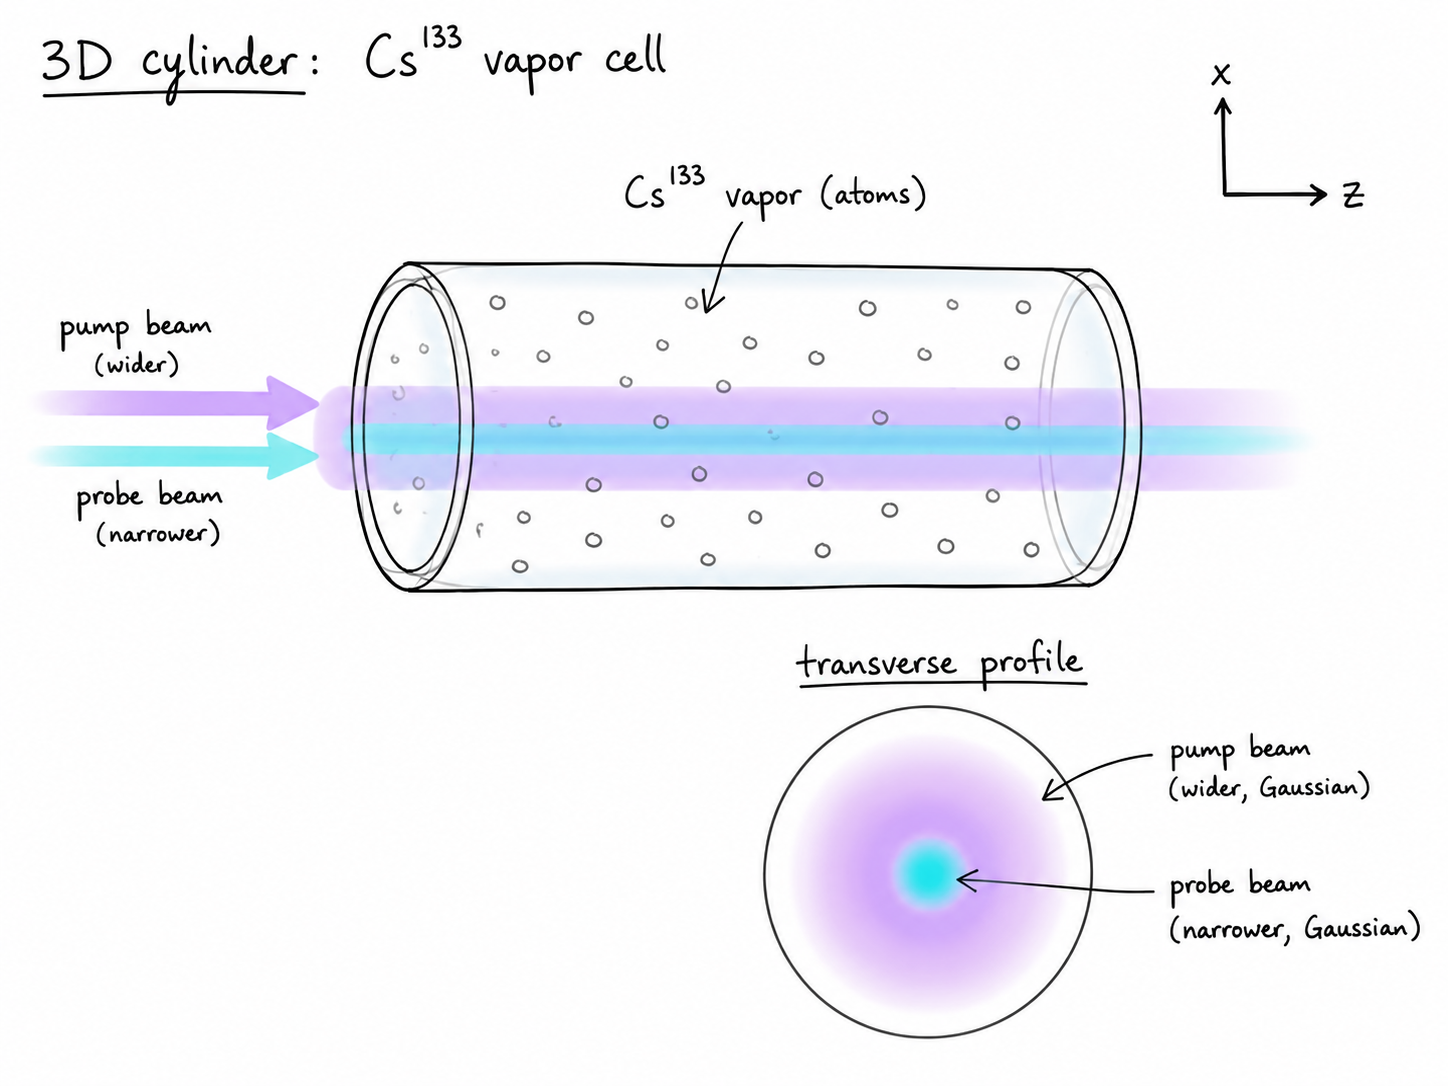
\includegraphics[width=0.72\textwidth]{Figures/ensemble_schematic.jpeg}
    \caption{Schematic representation of the reference warm-vapour geometry. The signal and control beams define a small optical interaction region inside the larger cylindrical vapour cell.}
    \label{fig:ensemble_schematic}
\end{figure}

This reference system is used as a validation case. The expected physical trends are already known: stronger confinement by buffer gas should slow motional loss, larger beams should increase the interaction time, magnetic-field gradients should produce phase dephasing, and phase mismatch should reduce directional retrieval. In this chapter, these expected trends are used to test whether the simulated quantity \(\mathcal{R}_{\mathrm{fib}}(t)\) behaves as a retrievable spin-wave mode.

\section{Directional Collective Emission}
\label{sec:results_directional_collective_emission}

The first validation test is the far-field emission pattern. During retrieval, the stored spin wave is converted into an optical polarization by the read control field. Each atom then contributes a small field amplitude, but the useful emission is not the incoherent sum of the emitted powers. It is the coherent sum of the fields. The direction in which these fields add constructively is fixed by the phase-matching condition~\cite{PsiL-odamIFm_GorshkovEtAl_2007},
\begin{equation}
    \mathbf{k}_{\mathrm{out}}
    =
    \mathbf{k}_{\mathrm{sig}}^{\mathrm{write}}
    -
    \mathbf{k}_{\mathrm{c}}^{\mathrm{write}}
    +
    \mathbf{k}_{\mathrm{c}}^{\mathrm{read}},
    \label{eq:results_phase_matching}
\end{equation}
where \(\mathbf{k}_{\mathrm{out}}\) is the retrieved optical wave vector, \(\mathbf{k}_{\mathrm{sig}}^{\mathrm{write}}\) is the signal wave vector during storage, and \(\mathbf{k}_{\mathrm{c}}^{\mathrm{write}}\) and \(\mathbf{k}_{\mathrm{c}}^{\mathrm{read}}\) are the write and read control-field wave vectors.

Figure~\ref{fig:far_field_angular_emission_profile} shows the simulated far-field angular distribution. The strongest emission is concentrated around the forward, phase-matched direction. This result is important because it confirms that the model is not simply tracking atomic survival. It is computing a collective interference pattern. The noise away from the central direction corresponds to residual constructive interference into other angular modes, but the dominant peak remains aligned with the expected retrieval direction.

\begin{figure}[htbp]
    \centering
    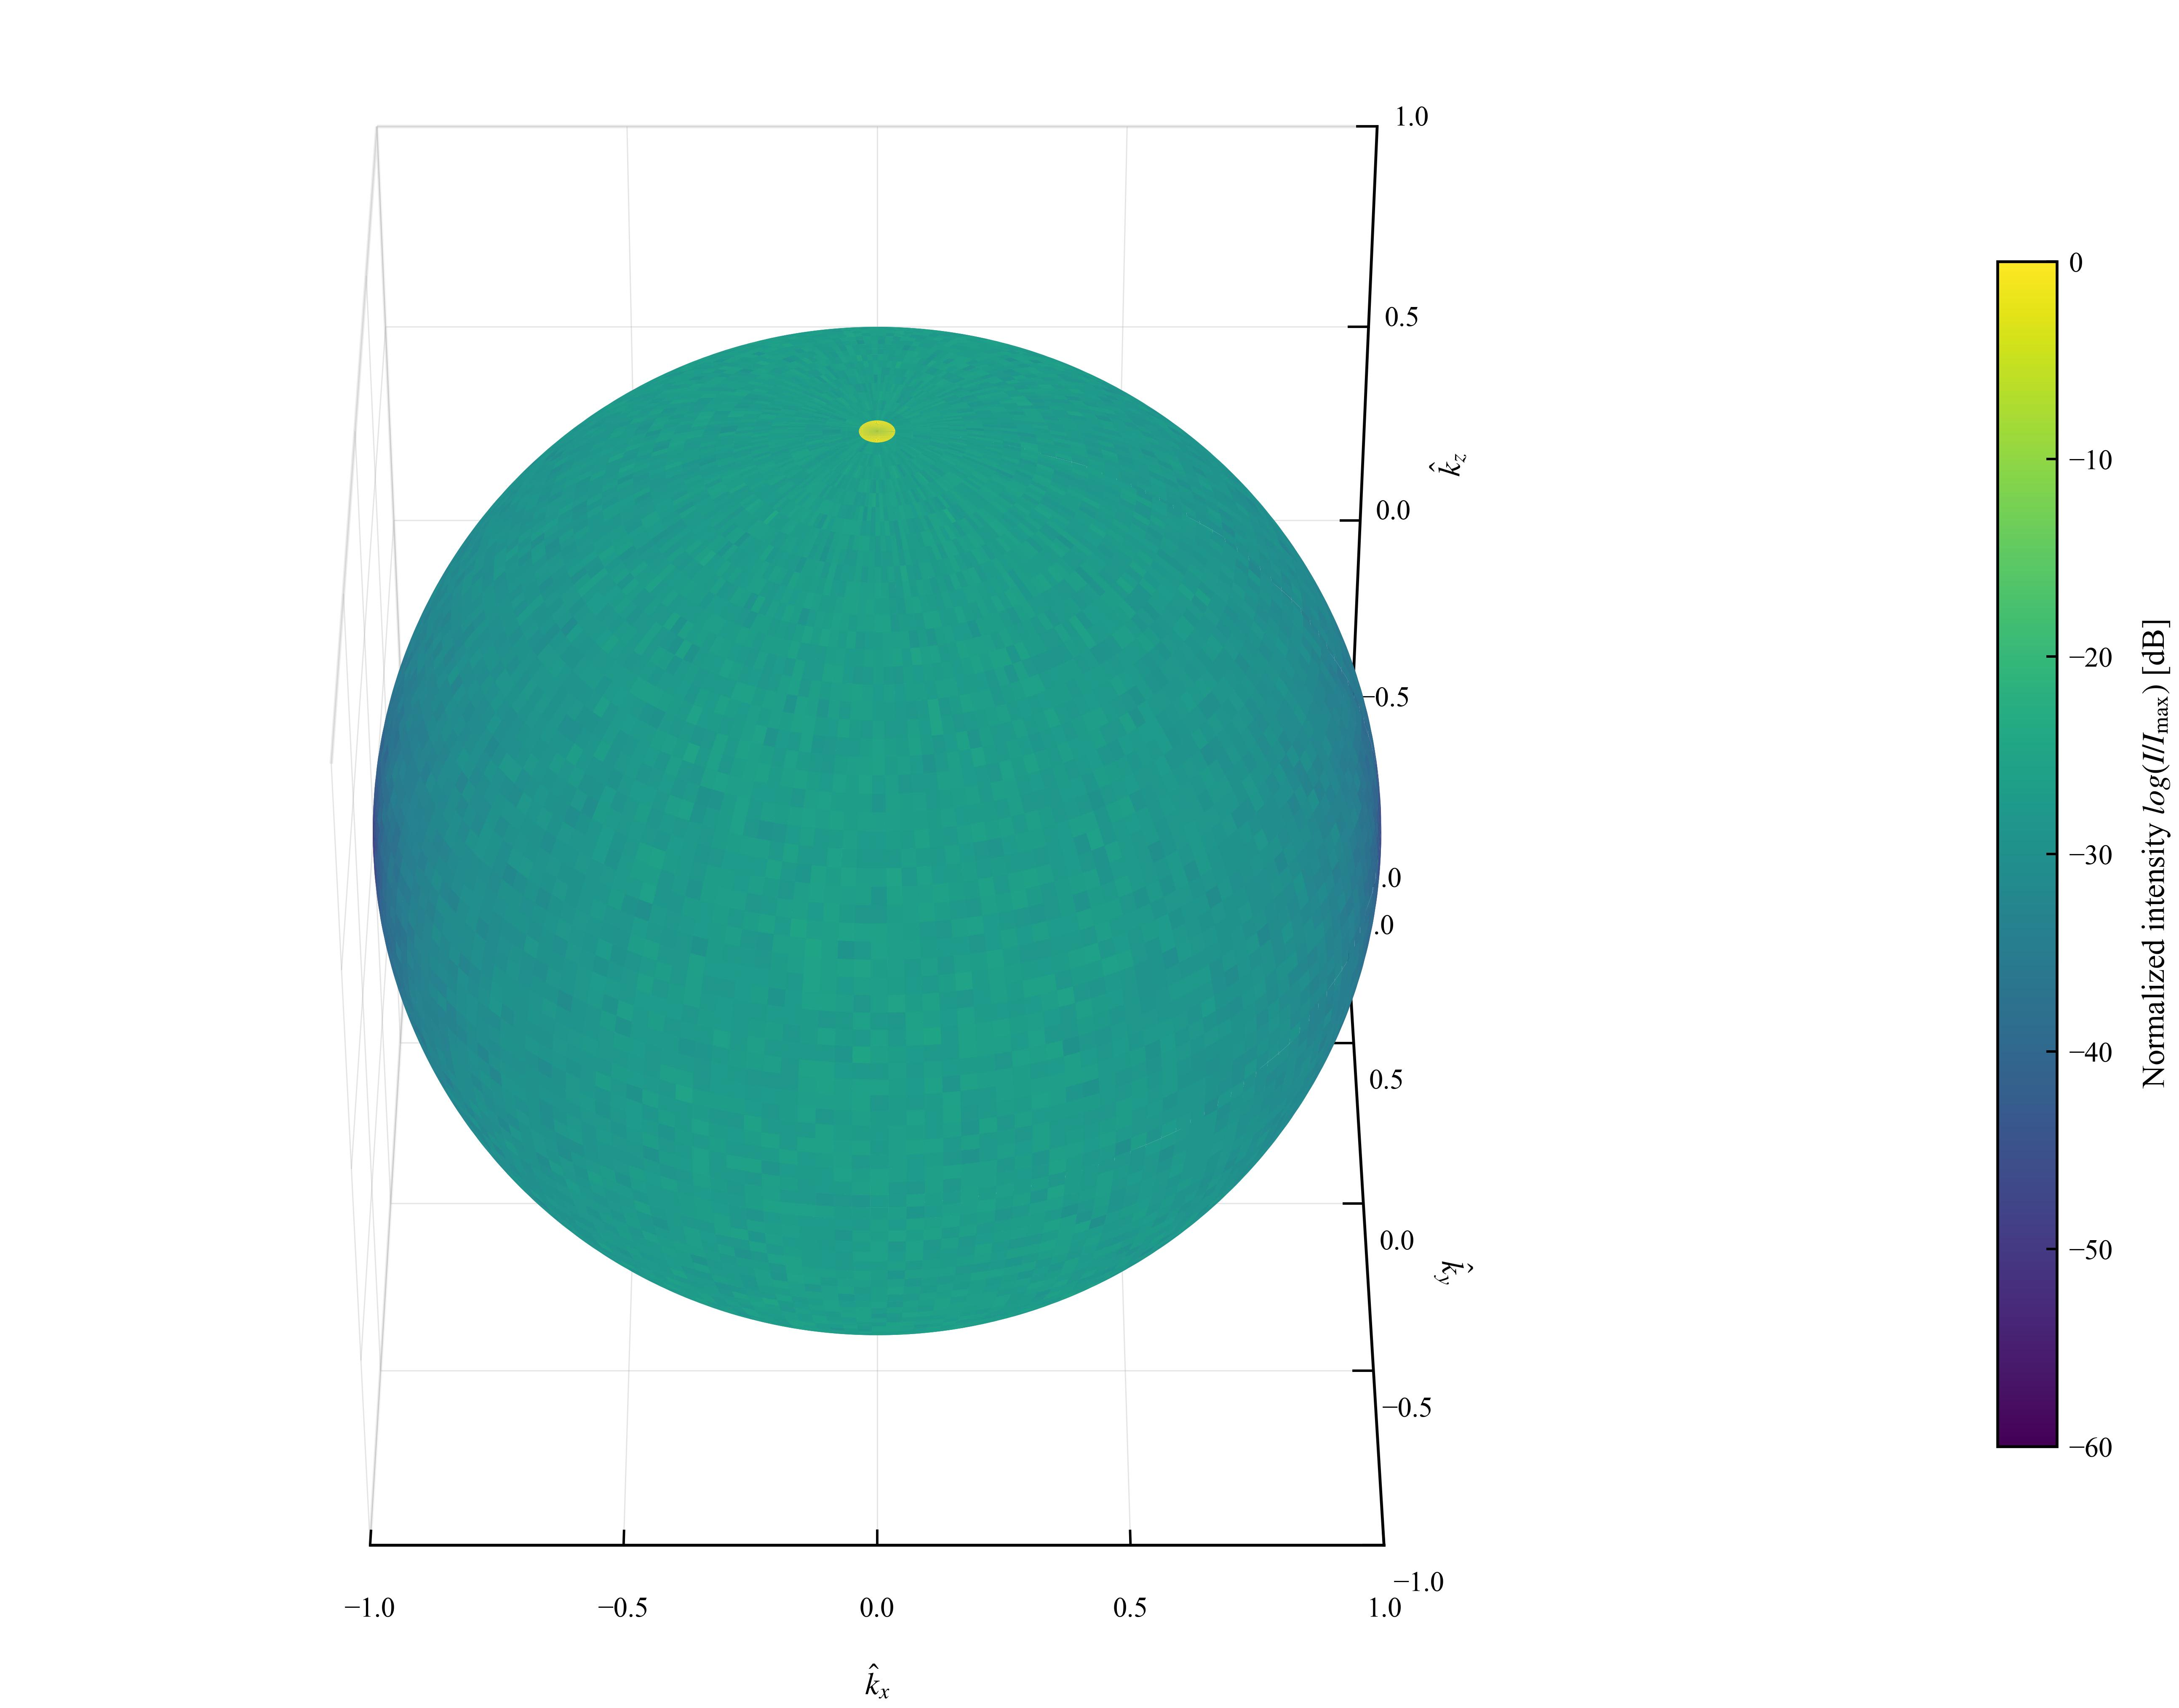
\includegraphics[width=0.70\textwidth]{Figures/far_field_angular_emission_profile.jpeg}
    \caption{Far-field angular emission profile obtained from the coherent dipole sum. The strongest emission appears in the forward phase-matched direction, validating that the simulated spin wave produces directional collective retrieval.}
    \label{fig:far_field_angular_emission_profile}
\end{figure}

The physical meaning of this result is simple. If the atomic phases are arranged according to the written spin wave, the emitted fields add in the direction selected by Eq.~\eqref{eq:results_phase_matching}. If the phases are randomized, the same atoms may still emit light, but the fields no longer add into the selected mode. Directional emission is therefore the first signature that the simulated observable is sensitive to the collective mode structure.

\section{Monte Carlo Convergence}
\label{sec:results_monte_carlo_convergence}

The second validation test concerns numerical convergence. Since the simulation samples a finite number of atoms and stochastic trajectories, the retrieved signal must be shown not to be dominated by rare events or sampling noise. For this reason, repeated Monte Carlo realizations are compared with the ensemble mean.

\begin{figure}[htbp]
    \centering
    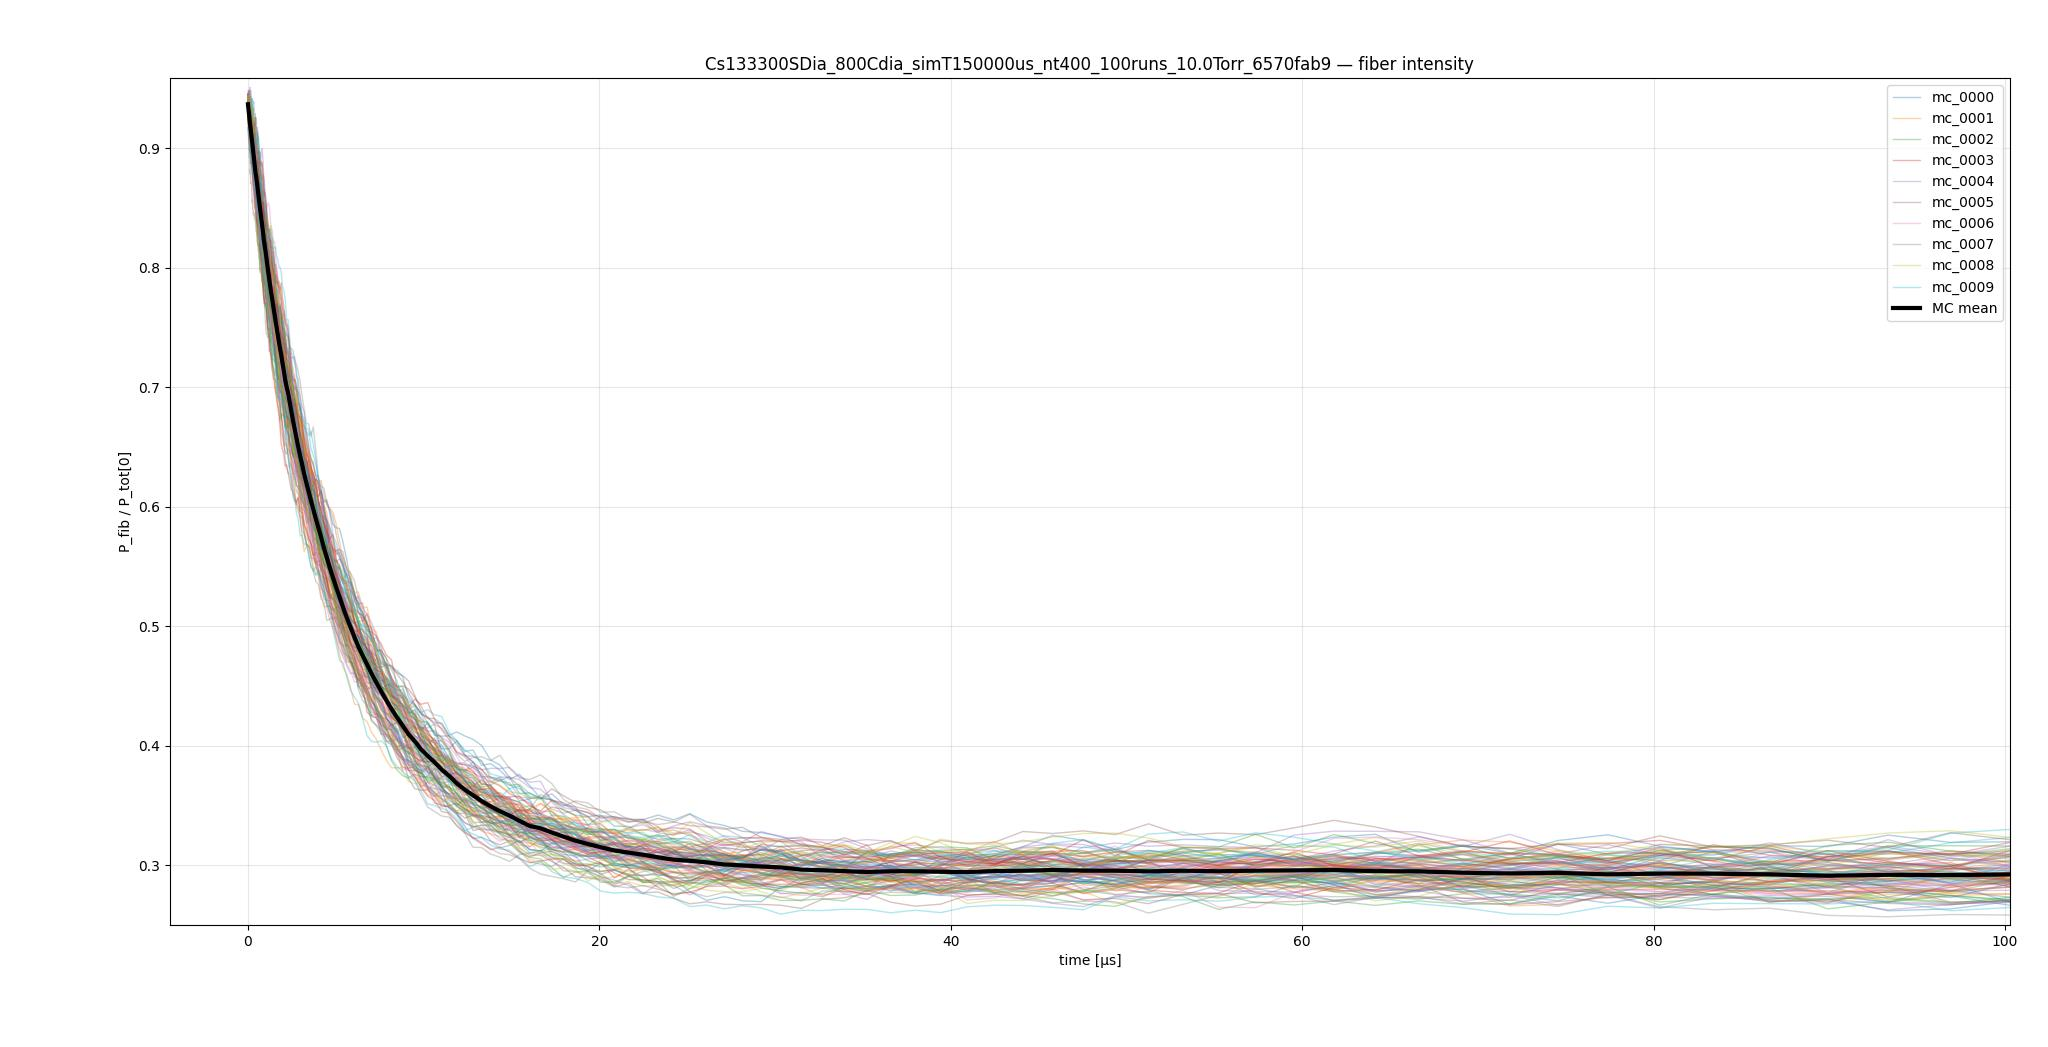
\includegraphics[width=0.72\textwidth]{Figures/monte_carlo_convergence.jpeg}
    \caption{Monte Carlo convergence of the normalized retrieved signal. Individual stochastic realizations follow the same global decay trend as the ensemble mean, showing that the simulated decay is not dominated by a small number of rare trajectories.}
    \label{fig:monte_carlo_convergence}
\end{figure}

Figure~\ref{fig:monte_carlo_convergence} shows that different realizations fluctuate around the same decay curve. The fluctuations are expected because the atoms follow different random trajectories, but the mean behaviour is stable. This validates the use of the Monte Carlo average as a numerical estimator of the retrieval-mode decay. The standard uncertainty of a simple Monte Carlo average decreases as the inverse square root of the number of independent samples~\cite{MonteCarloNotes}. Increasing the number of simulated atoms therefore improves the smoothness of the retrieved decay curve, but does not change the physical trend once convergence has been reached.

\section{Gas-Phase Transport and Buffer-Gas Pressure}
\label{sec:results_buffer_gas_pressure}

After the collective emission and numerical convergence have been validated, the first physical parameter scan is the buffer-gas pressure. Buffer gas changes the motion of alkali atoms by producing frequent velocity-changing collisions. In a warm vapour without sufficient confinement, atoms carrying the spin-wave coherence leave the high-overlap optical mode on a transit-time scale. Once they leave this region, their contribution to \(P_{\mathrm{fib}}(t)\) is reduced even if their internal ground-state coherence has not been completely destroyed.

The diffusion model captures this effect through the diffusion coefficient \(D\). Larger buffer-gas pressure reduces the diffusion coefficient and therefore slows the spatial escape of atoms from the signal and control beam volume. The expected result is a slower decay of \(\mathcal{R}_{\mathrm{fib}}(t)\).

\begin{figure}[htbp]
    \centering
    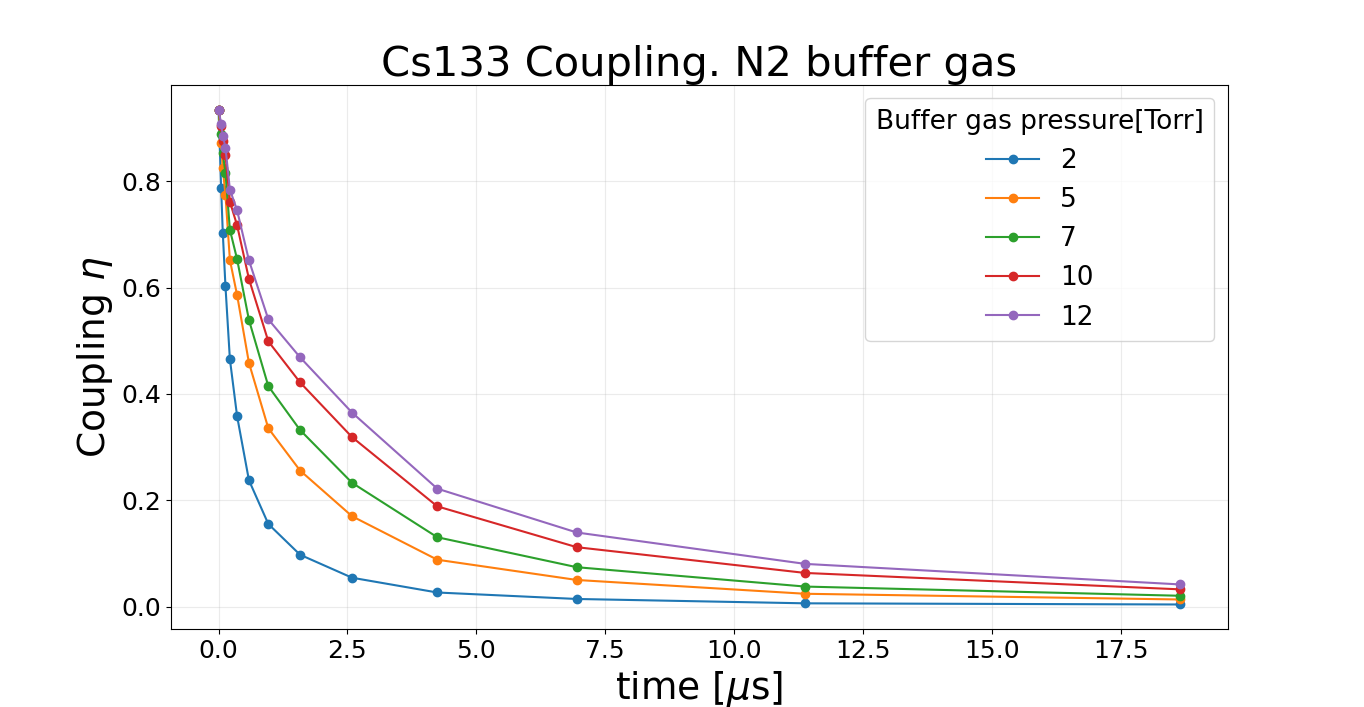
\includegraphics[width=0.72\textwidth]{Figures/pressure_scan_coupling_decay.jpeg}
    \caption{Pressure scan of the normalized fibre-coupled retrieval. Increasing the buffer-gas pressure reduces atomic diffusion and extends the time over which atoms remain inside the high-overlap optical mode.}
    \label{fig:pressure_scan_coupling_decay}
\end{figure}

Figure~\ref{fig:pressure_scan_coupling_decay} shows this behaviour. At lower pressure, the retrieval decays more rapidly because atoms diffuse away from the spatial region where the stored spin wave overlaps well with the readout mode. At higher pressure, the motion is slowed, and the collective mode survives for a longer time. The result should be interpreted as a mode-overlap effect. The atoms are not necessarily destroyed when they leave the beam. Rather, their phase and position no longer match the mode that can radiate efficiently back into the fibre.

\section{Beam-Size Dependence}
\label{sec:results_beam_size}

The same physical mechanism can be tested by changing the optical beam sizes. A larger beam defines a larger interaction region. An atom must move farther before its contribution to the signal-control overlap becomes small. Thus, increasing the signal or control beam size should increase the decay time of the retrieved mode.

\begin{figure}[htbp]
    \centering
    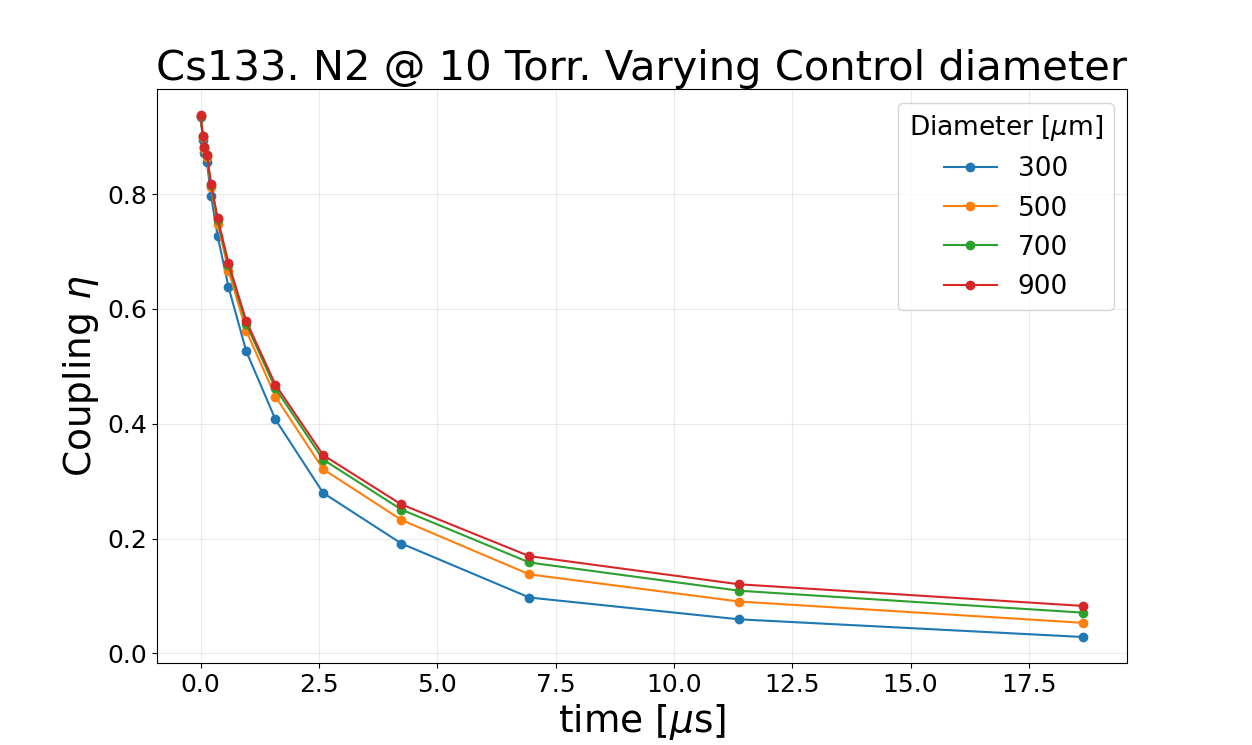
\includegraphics[width=0.72\textwidth]{Figures/beam_size_scan_coupling_decay.jpeg}
    \caption{Beam-size dependence of the normalized retrieval. Larger signal or control beams increase the spatial region over which atoms remain coupled to the readout mode, leading to a slower decay of \(P_{\mathrm{fib}}(t)/P_{\text{tot}}(0)\).}
    \label{fig:beam_size_scan_coupling_decay}
\end{figure}

Figure~\ref{fig:beam_size_scan_coupling_decay} confirms this trend. Larger beams give a longer coupling time because the stored spin wave is distributed over a wider transverse region. The decay is therefore less sensitive to short diffusive displacements. This result is consistent with the usual warm-vapour intuition that transit-time broadening is reduced when the optical mode is enlarged~\cite{Apgteitiav_FinkelsteinEtAl_2023}.

However, this improvement is not a free optimization. In an experiment, increasing the beam size can reduce optical intensity for fixed power, modify the EIT bandwidth, and change the optical depth sampled by the mode. These effects are not fully included in the present simulation. The result here should therefore be read as a statement about spatial mode survival: for fixed optical preparation, a larger beam makes the retrievable spin-wave mode less sensitive to atomic motion.

\section{Comparison with a Cold Gaussian Ensemble}
\label{sec:results_bec_comparison}

The same beam-size logic was also tested in a cold Gaussian ensemble. The simulated cloud contains \(10^8\) atoms with a Gaussian spatial distribution of width approximately \(\SI{1}{\milli\metre}\). The control and signal beams are taken to be smaller than the cloud, so that the stored mode is still defined by the optical overlap rather than by the full atom distribution.

\begin{figure}[htbp]
    \centering
    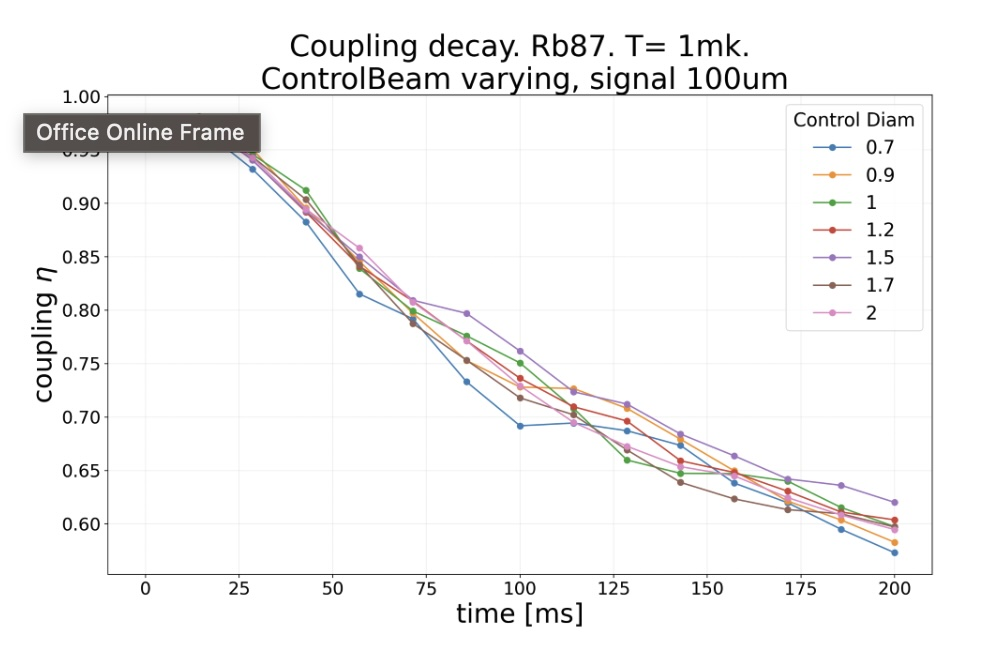
\includegraphics[width=0.72\textwidth]{Figures/bec_beam_size_scan.jpeg}
    \caption{Beam-size scan for a cold Gaussian ensemble. The same qualitative increase in coupling time is observed when the optical mode is enlarged, although the effect is weaker than in the warm-vapour reference case because thermal diffusion is no longer the dominant limitation.}
    \label{fig:bec_beam_size_scan}
\end{figure}

Figure~\ref{fig:bec_beam_size_scan} shows that increasing the beam size also increases the coupling time in the cold-cloud case, but the change is less pronounced than in the warm-vapour cell. This is expected. In the warm vapour, atoms move rapidly through the optical mode, so the transverse beam size directly controls the escape time. In the cold ensemble, the motion is slower and the dominant limitation is no longer the same diffusive transit through the beam. The result is useful because it shows that the same retrieval-overlap formalism can be applied to different atomic platforms, while the dominant physical mechanism changes.

\section{Geometric Phase Mismatch from Control-Beam Angle}
\label{sec:results_control_beam_angle}

A change in the relative angle between the signal and control fields changes the spin-wave wave vector,
\begin{equation}
    \Delta\mathbf{k}
    =
    \mathbf{k}_{\mathrm{sig}}
    -
    \mathbf{k}_{\mathrm{c}},
    \label{eq:results_delta_k_angle}
\end{equation}
where \(\mathbf{k}_{\mathrm{sig}}\) and \(\mathbf{k}_{\mathrm{c}}\) are the signal and control wave vectors during storage. Even a small angular mismatch introduces a transverse spin-wave phase gradient. This matters because atoms that move transversely through this phase grating accumulate different phases. If the spin-wave period is short, a small displacement is enough to change the phase significantly. If the spin-wave period is long, the same displacement produces a smaller phase error.

\begin{figure}[htbp]
    \centering
    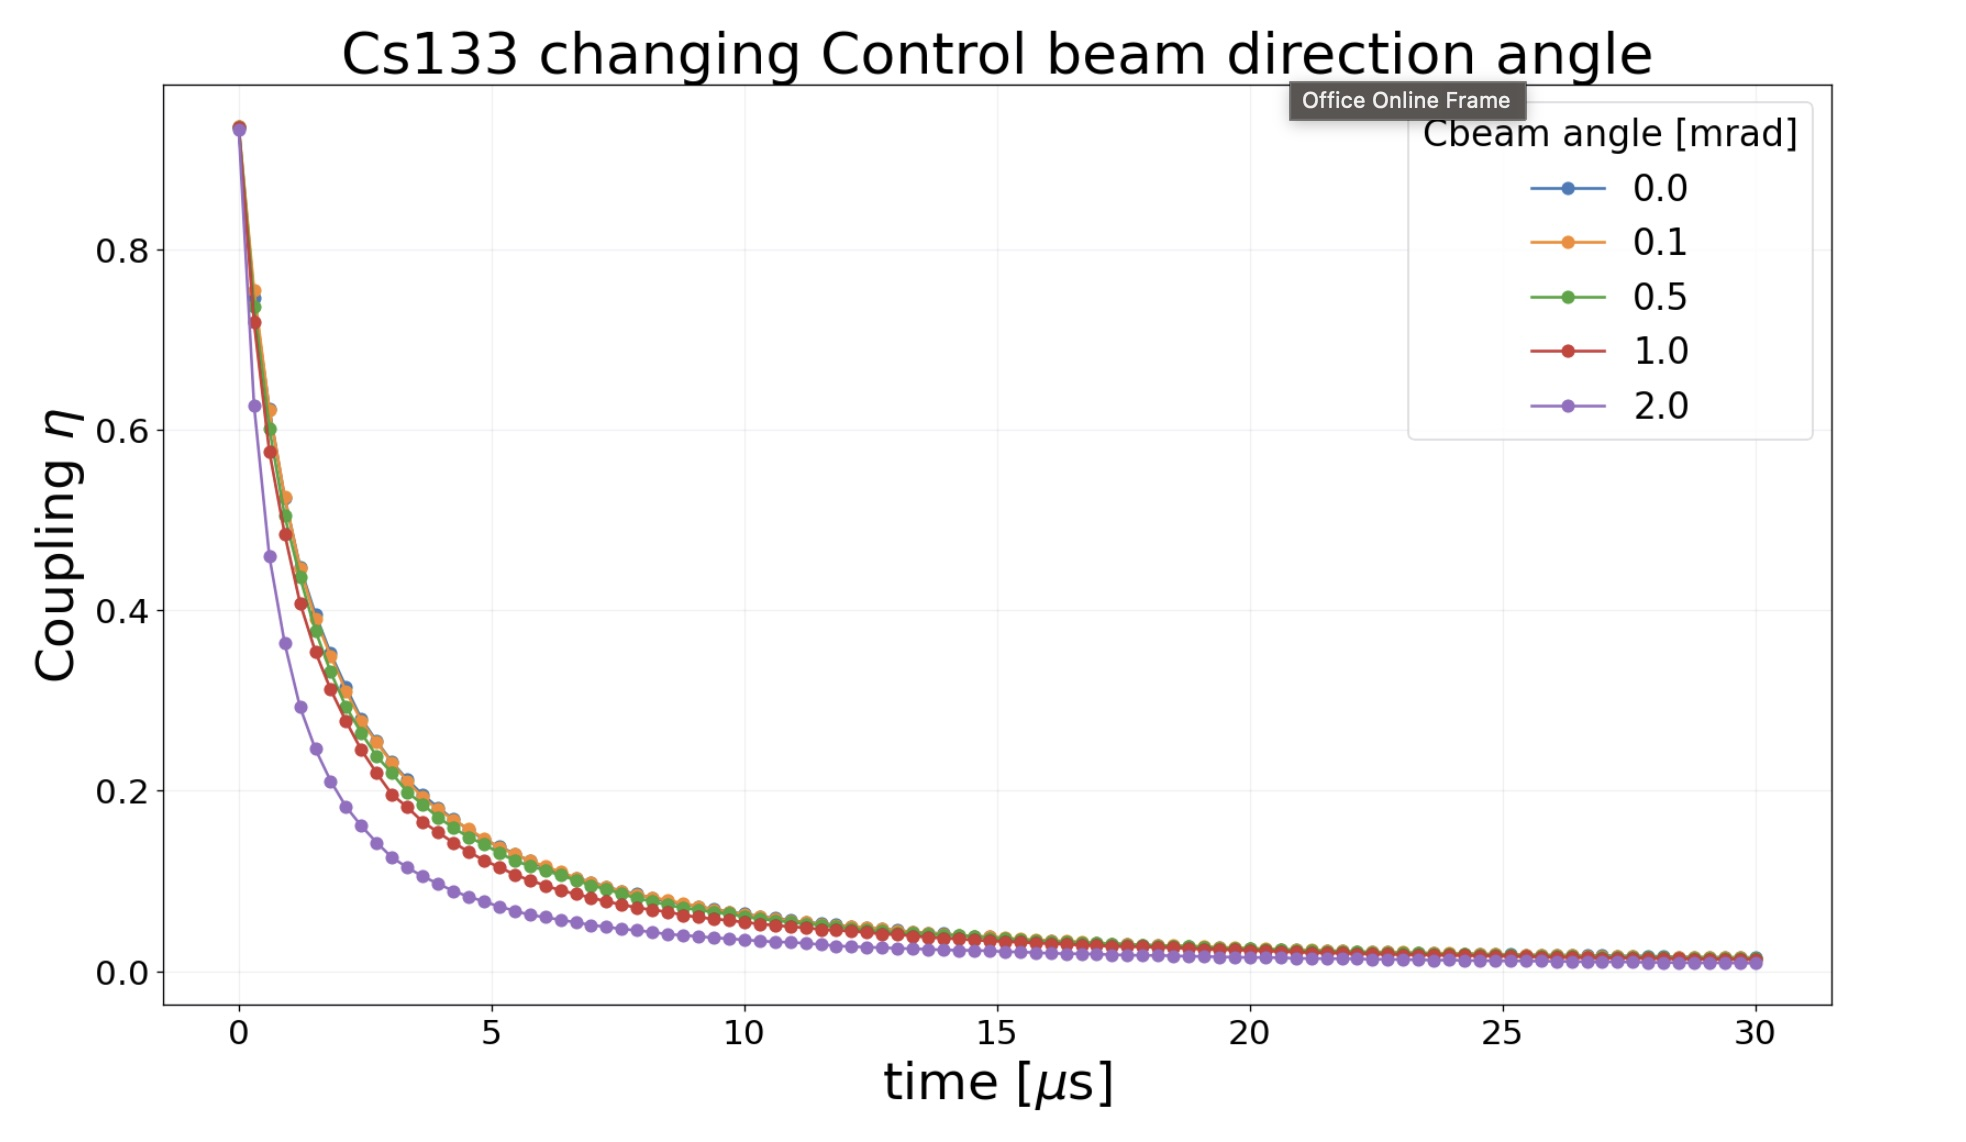
\includegraphics[width=0.72\textwidth]{Figures/control_beam_angle_scan.jpeg}
    \caption{Control-beam angle scan. Changing the signal-control angle modifies the spin-wave wave vector and therefore the sensitivity of the stored coherence to atomic motion.}
    \label{fig:control_beam_angle_scan}
\end{figure}

Figure~\ref{fig:control_beam_angle_scan} shows the effect of this geometric phase mismatch. The retrieved mode decays faster when the spin-wave phase varies more rapidly across the ensemble. This is not a loss of atoms; it is a loss of relative phase. The atoms can still carry ground-state coherence, but the spatial phase pattern no longer matches the phase-matched readout mode.

This result is especially important for warm-vapour EIT, where signal and control beams are usually kept nearly co-propagating. Small relative angles can broaden the two-photon resonance and introduce motional dephasing because the effective two-photon wave vector becomes nonzero~\cite{Apgteitiav_FinkelsteinEtAl_2023}. The simulation reproduces this intuition at the level of the retrievable spin-wave mode.

\section{Magnetic-Gradient Dephasing}
\label{sec:results_magnetic_gradient}

A magnetic-field gradient provides a different way to destroy the collective mode. Instead of changing the optical phase written into the spin wave, it makes the ground-state splitting position dependent. The accumulated phase of atom \(j\) may be written as
\begin{equation}
    \phi_j(t)
    =
    \int_0^t
    \omega_{sg}\!\left(\mathbf{r}_j(t')\right)
    \,dt',
    \label{eq:results_magnetic_phase}
\end{equation}
where \(\omega_{sg}(\mathbf{r})\) is the local angular frequency splitting between \(\ket{g}\) and \(\ket{s}\), and \(t'\) is the integration variable. If \(\omega_{sg}\) is the same everywhere, all atoms acquire the same phase and the collective interference is unchanged. If \(\omega_{sg}\) varies across the cell, different atoms acquire different phases, and the collective readout is reduced.

\begin{figure}[htbp]
    \centering
    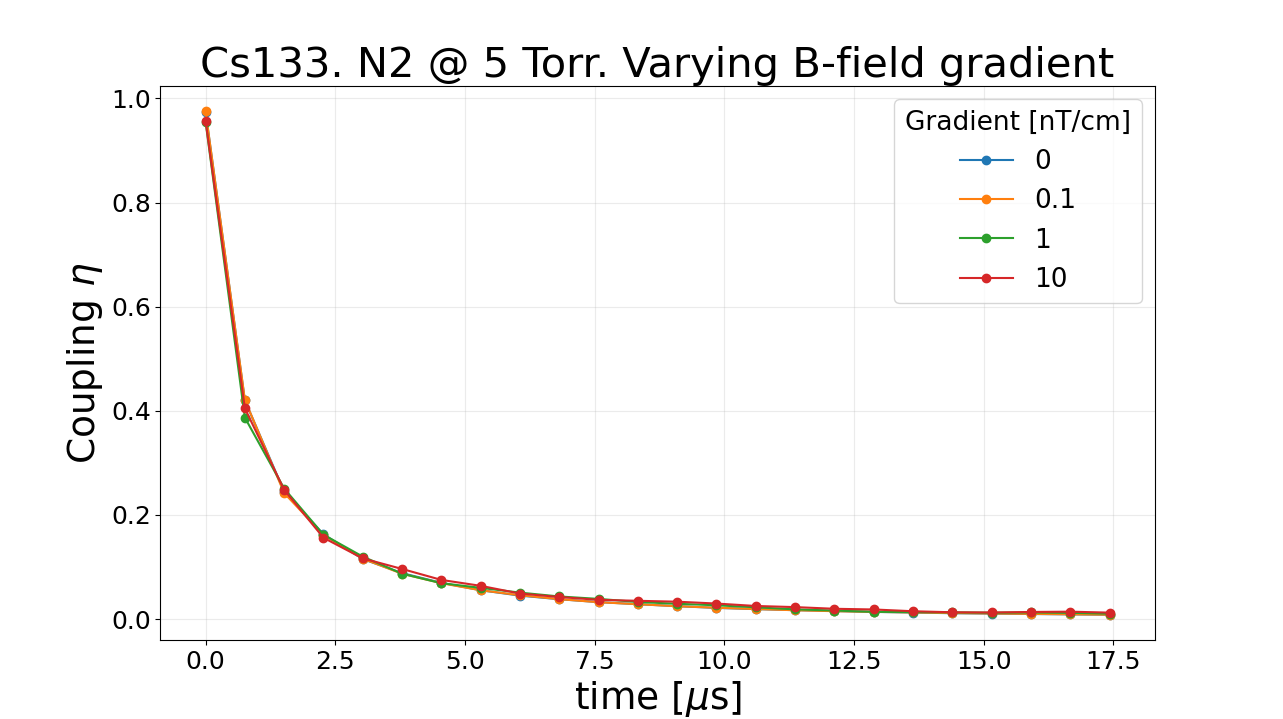
\includegraphics[width=0.72\textwidth]{Figures/magnetic_gradient_scan.jpeg}
    \caption{Magnetic-gradient-induced decay of the normalized retrieval. A spatially varying ground-state splitting causes atoms in different parts of the ensemble to accumulate different phases, reducing constructive retrieval into the target mode.}
    \label{fig:magnetic_gradient_scan}
\end{figure}

Figure~\ref{fig:magnetic_gradient_scan} shows that increasing the magnetic gradient accelerates the decay of \(P_{\mathrm{fib}}(t)/P_{\text{tot}}(0)\). The physical mechanism is phase scrambling. Unlike beam-size loss, where atoms leave the optical mode, magnetic dephasing can reduce retrieval even when the atoms remain inside the beam. This distinction is useful experimentally because the two mechanisms require different improvements. Beam-size or buffer-gas changes address spatial escape, while magnetic shielding and field homogeneity address phase evolution.

\section{Compact-Cell Geometry}
\label{sec:results_compact_cell_geometry}

The reference cell is long compared with its optical mode and has a diameter much larger than the beam waist. In that regime, atoms can diffuse out of the optical mode before wall collisions dominate the retrieval decay. The compact geometry changes this balance. The simulated compact cell has diameter \(\SI{1}{\milli\metre}\) and length \(\SI{10}{\milli\metre}\), with control and signal FWHM diameters of approximately \(\SI{0.8}{\milli\metre}\) and \(\SI{0.3}{\milli\metre}\), respectively. The optical mode now occupies a substantial fraction of the cell cross-section.

This changes the interpretation of the decay. In the reference geometry, an atom can leave the optical mode while still being far from the cell boundary. In the compact geometry, the cell wall is close to the optical mode. Atoms that carry the spin-wave coherence therefore reach the wall on timescales relevant for the simulated retrieval decay. The boundary condition can no longer be ignored.

\section{Wall Coatings as an Effective Boundary Condition}
\label{sec:results_wall_coatings}

The wall interaction has two parts that must be kept conceptually separate. The first is mechanical reflection: the atom remains inside the cell after hitting the boundary. The second is internal-state survival: the atom may or may not retain the ground-state coherence that allows it to contribute to the spin wave. These two processes are not the same. An atom can return to the vapour mechanically while its spin coherence has already been randomized by the surface interaction~\cite{OP_Happer_1972}.

The simulation represents the coating as an effective survival probability per wall collision. If \(N_{\text{b}}\) is the average number of wall collisions before depolarization, the survival probability per collision is written as
\begin{equation}
    p_{\mathrm{survive}}
    =
    1-\frac{1}{N_{\text{b}}},
    \label{eq:results_wall_survival_probability}
\end{equation}
where \(p_{\mathrm{survive}}\) is the probability that the atomic ground-state coherence survives one wall encounter. This model does not describe the microscopic chemistry of the coating. Instead, it condenses the complicated surface interaction into a single effective parameter.

Anti-relaxation coatings are useful because they reduce the probability that a wall encounter destroys the atomic spin state. The detailed coating performance depends on material, temperature, surface coverage, adsorption dynamics, and morphology~\cite{Aiacoavc_ChiEtAl_2020}. For the compact-cell simulations, this complexity is represented by scanning \(N_{\text{b}}\). Small \(N_{\text{b}}\) corresponds to a poor coating or nearly depolarizing wall. Large \(N_{\text{b}}\) corresponds to a wall that preserves coherence over many collisions.

\begin{figure}[htbp]
    \centering
    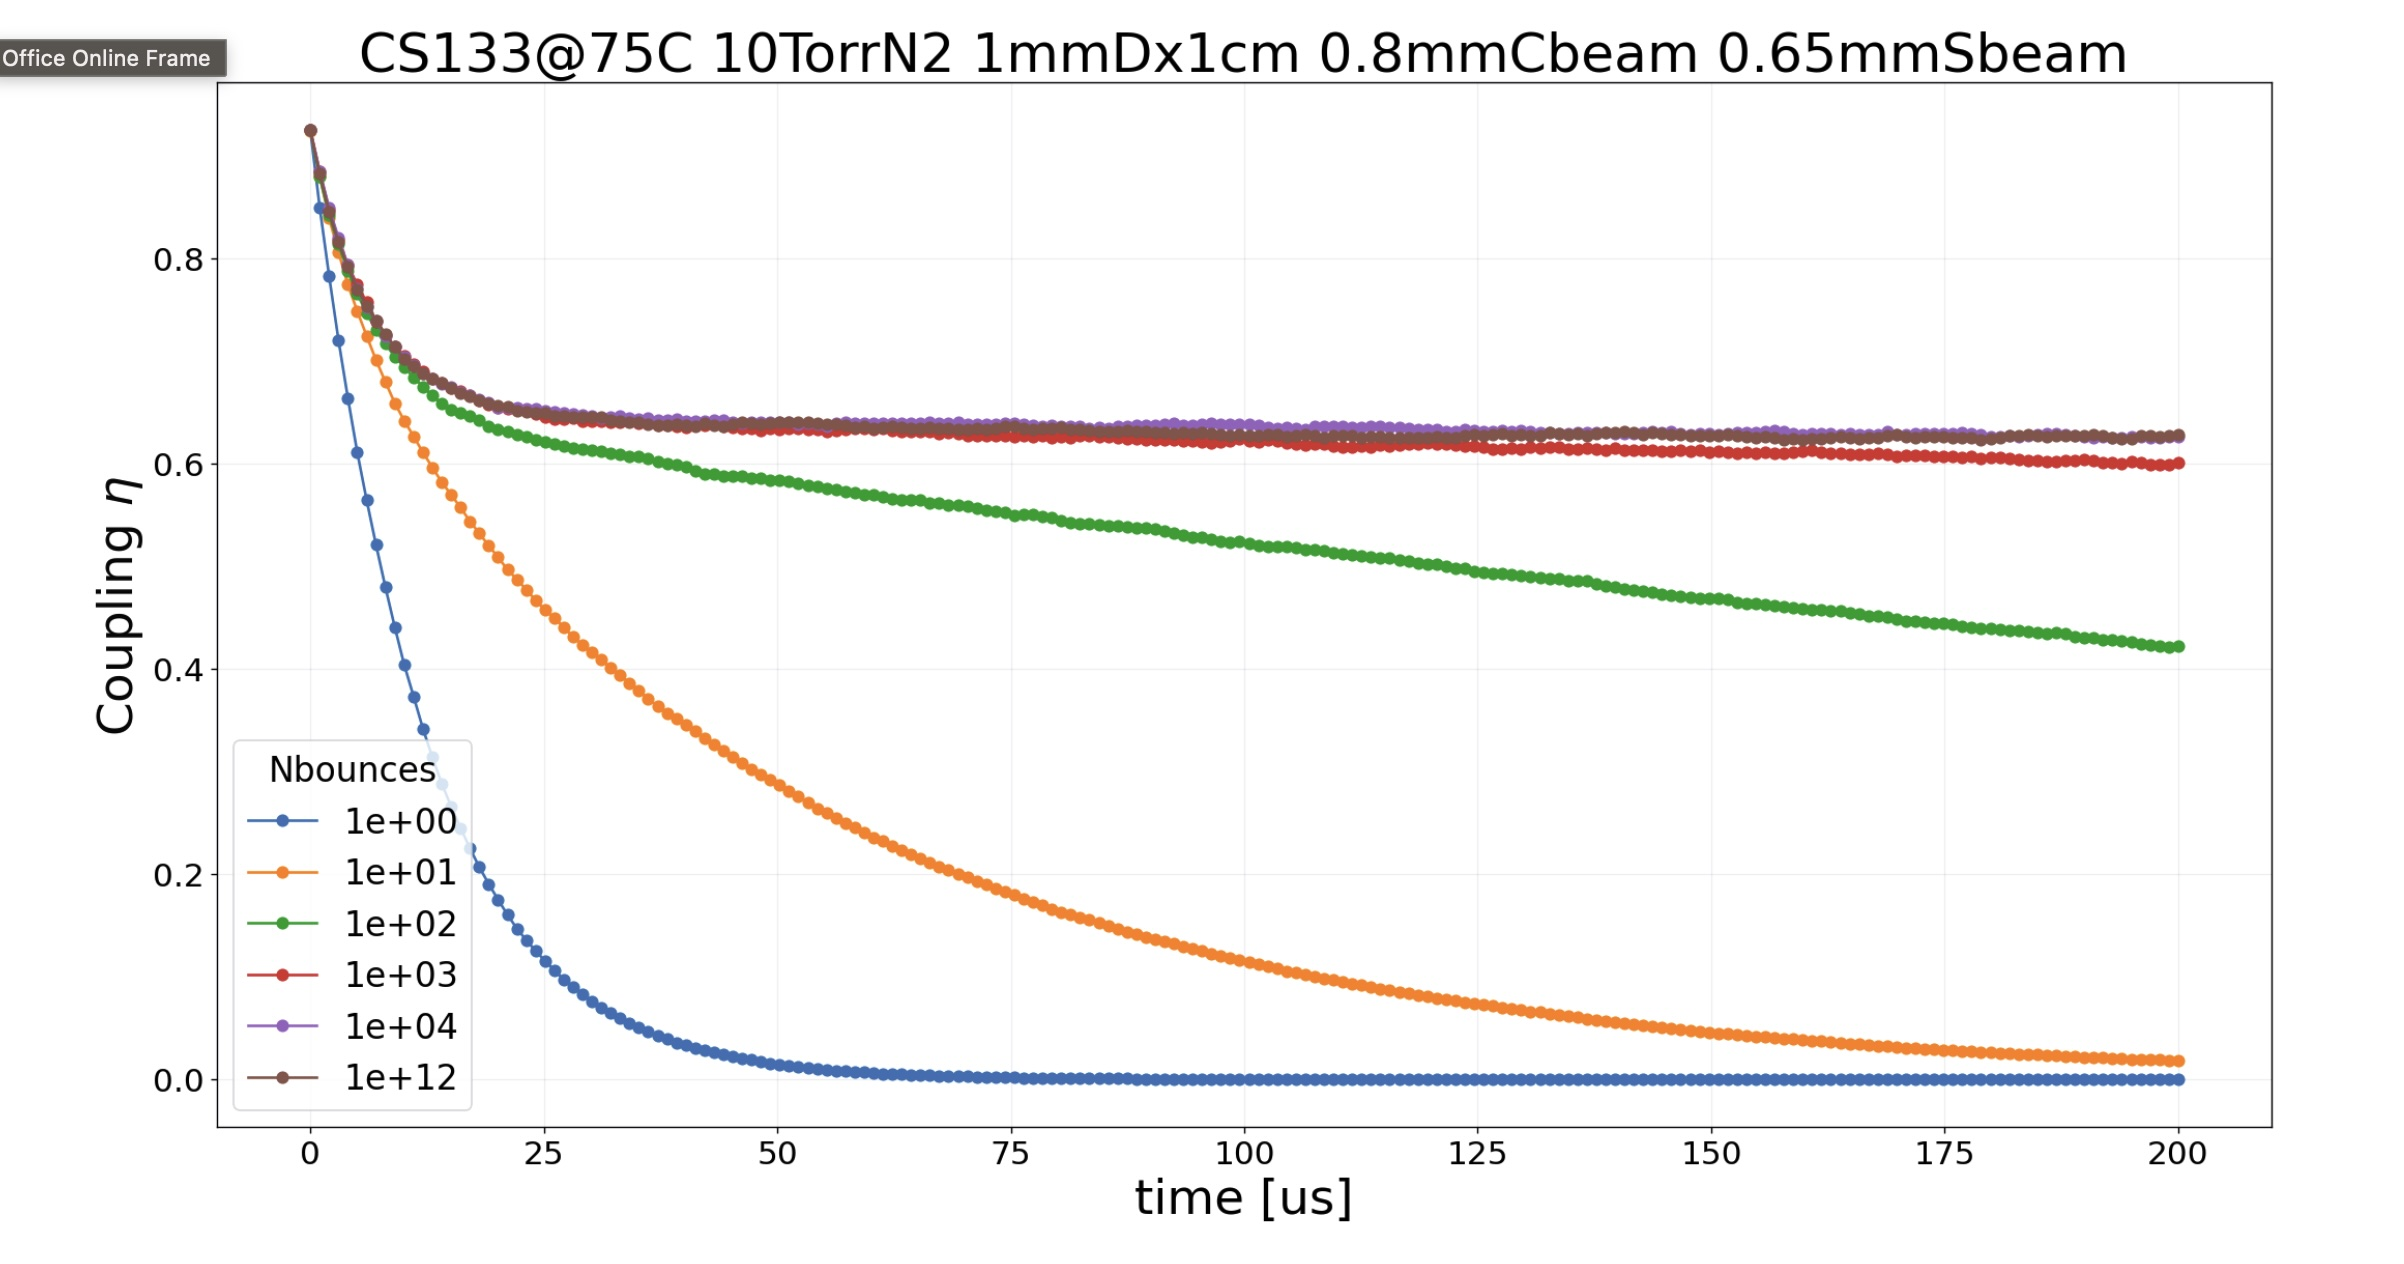
\includegraphics[width=0.72\textwidth]{Figures/coating_bounce_scan.jpeg}
    \caption{Compact-cell coating scan. Increasing the average number of coherence-preserving wall collisions \(N_{\text{b}}\) improves the retrieval decay when wall relaxation is the dominant loss channel.}
    \label{fig:coating_bounce_scan}
\end{figure}

Figure~\ref{fig:coating_bounce_scan} shows that increasing \(N_{\text{b}}\) improves the retrieval lifetime for poor coatings. In this regime, each wall encounter has a significant probability of removing the atom from the collective spin wave, so wall collisions act almost like an absorbing boundary for the retrievable mode. When \(N_{\text{b}}\) is increased, atoms can hit the wall and return to the vapour while still carrying coherence. The retrieved signal therefore decays more slowly.

The improvement does not continue indefinitely. Once \(N_{\text{b}}\) is large enough, the curves begin to converge. In that regime, wall-induced depolarization is no longer the dominant limitation. The remaining decay is set mainly by diffusion through the optical mode, the finite cell geometry, and imperfect overlap with the readout mode. This saturation is an important design result: beyond a certain coating quality, improving the wall survival alone does not strongly increase \(P_{\mathrm{fib}}(t)/P_{\text{tot}}(0)\).

\section{Temperature Dependence in the Compact Cell}
\label{sec:results_temperature_compact_cell}

Temperature affects a warm-vapour memory in two opposite ways. Increasing the temperature raises the alkali vapour pressure and can increase the optical depth, which is beneficial for storage and retrieval efficiency. At the same time, higher temperature increases the thermal velocity and modifies the transport through the buffer gas. It can also make wall interactions and coating stability more important~\cite{Apgteitiav_FinkelsteinEtAl_2023,Aiacoavc_ChiEtAl_2020}.

The present simulation focuses on the transport and mode-overlap side of this trade-off. It does not compute the full temperature dependence of the EIT optical depth. Therefore, the temperature scan should not be read as a complete optimization of memory efficiency. It should be read as a test of how motion and wall encounters affect the retrievable spin-wave mode under different thermal conditions.

\begin{figure}[htbp]
    \centering
    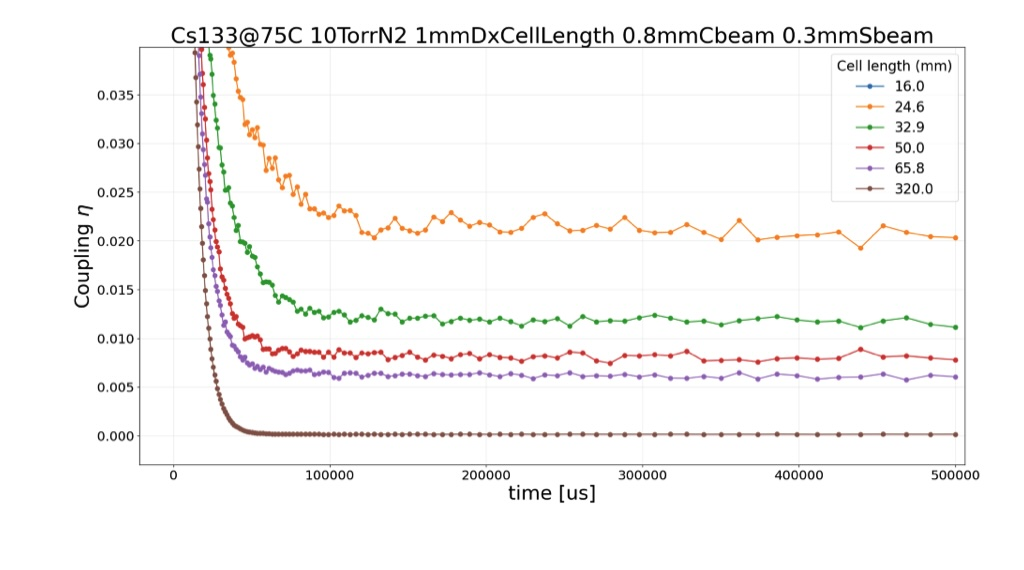
\includegraphics[width=0.72\textwidth]{Figures/compact_temperature_scan.jpeg}
    \caption{Temperature dependence of the compact-cell retrieval for different wall-survival parameters. The plotted decay reflects the transport and wall-relaxation contribution to the retrievable-mode lifetime, not the full optical-depth optimization of an EIT memory.}
    \label{fig:compact_temperature_scan}
\end{figure}

Figure~\ref{fig:compact_temperature_scan} shows the resulting temperature-dependent retrieval decay. When the wall survival is low, the decay is strongly affected by the rate at which atoms reach the boundary. When the wall survival is high, the decay becomes less sensitive to the coating parameter and more sensitive to residual mode-overlap loss. This is the regime in which atoms may survive wall encounters but still fail to return with the correct spatial phase and optical overlap for efficient fibre-coupled retrieval.

\section{Cell Length and Spin-Wave Phase}
\label{sec:results_cell_length_spin_wave}

The compact-cell geometry also makes the relationship between cell length and spin-wave phase important. The stored spin wave contains a phase factor
\begin{equation}
    e^{i\Delta\mathbf{k}\cdot\mathbf{r}},
    \label{eq:results_spin_wave_phase_factor}
\end{equation}
where \(\Delta\mathbf{k}\) is set by the signal-control geometry. If the cell length is short compared with the spin-wave period, the phase does not vary strongly across the cell. If the cell spans many spin-wave periods, different longitudinal regions of the cell can contribute with very different phases.

\begin{figure}[htbp]
    \centering
    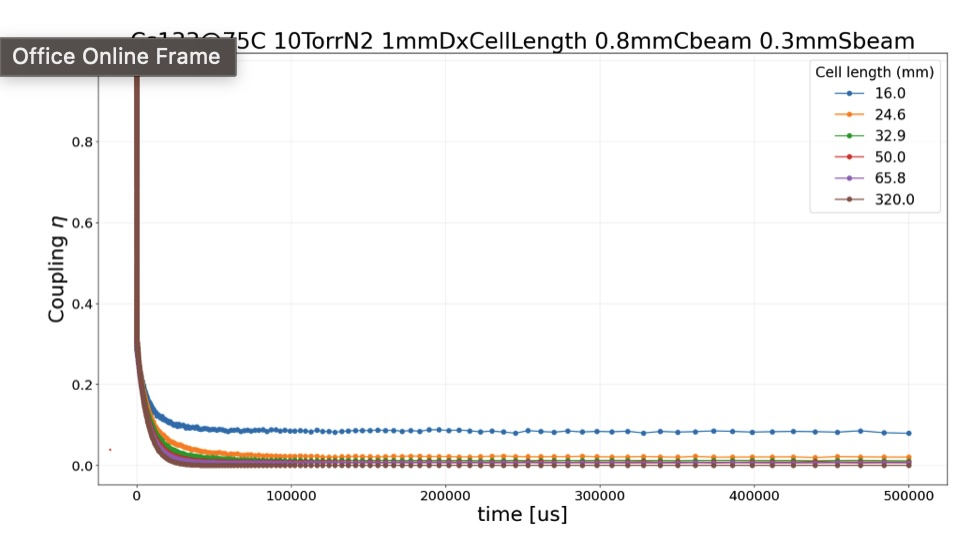
\includegraphics[width=0.72\textwidth]{Figures/cell_length_spin_wave_scan.jpeg}
    \caption{Cell-length scan relative to the spin-wave phase period. When the cell length spans many spin-wave periods, different parts of the ensemble contribute with different phases, reducing the retrievable collective mode.}
    \label{fig:cell_length_spin_wave_scan}
\end{figure}

Figure~\ref{fig:cell_length_spin_wave_scan} shows that the long-time plateau is sensitive to the relation between cell length and spin-wave phase. This result should not be interpreted as a simple volume effect. A longer cell contains more atoms, but it also samples more of the spin-wave phase pattern. If the phase varies significantly over the cell, the coherent sum into the target mode can decrease because different regions interfere less constructively.

This effect is especially relevant when comparing compact and elongated geometries. Miniaturization does not only change the wall-collision rate. It also changes how much of the spin-wave phase structure is sampled by the ensemble and how this structure overlaps with the readout mode.

%\chapter{Optimisation of Experimental Parameters}
\label{chap:experimental_optimisation}

The previous chapter considered intrinsic platform properties that are fixed once the system has been fabricated or purchased. This chapter instead examines experimentally adjustable parameters that can be modified during operation. The influence of the optical beam dimensions, beam geometry, and magnetic-field homogeneity is evaluated through their effect on the fibre-coupled retrieval.

\section{Optical Beam Geometry}
\label{sec:results_optical_beam_geometry}

The optical geometry determines both the spatial extent of the prepared spin wave and the phase-matching conditions for retrieval. The beam widths and relative propagation directions are therefore considered separately.

\subsection{Beam Width}
\label{sec:results_beam_width}

The signal and control fields are represented by Gaussian transverse profiles whose diameters can be modified through the optical focusing system. Changing the beam widths alters the number of atoms contributing significantly to the prepared and retrieved modes, as well as the distance that an atom must travel before its optical weight becomes small.

A wider interaction region reduces the sensitivity to transverse atomic motion. In the warm-vapour system, diffusing atoms must travel farther before leaving the region of significant mode overlap. In the cold-atom system, a larger mode similarly increases the ballistic transit time across the illuminated region. For fixed atomic preparation and transport parameters, increasing the beam width is therefore expected to extend the decay time of the fibre-coupled retrieval.

The comparison between the warm-vapour and cold-atom systems is shown in Fig.~\ref{fig:beam_width_scan}. Although the transport mechanisms differ, the same geometric effect is observed in both platforms. Larger optical modes remain overlapped with the moving ensemble for longer times and consequently produce a slower reduction of the retrieved signal.

\begin{figure}[htbp]
    \centering
        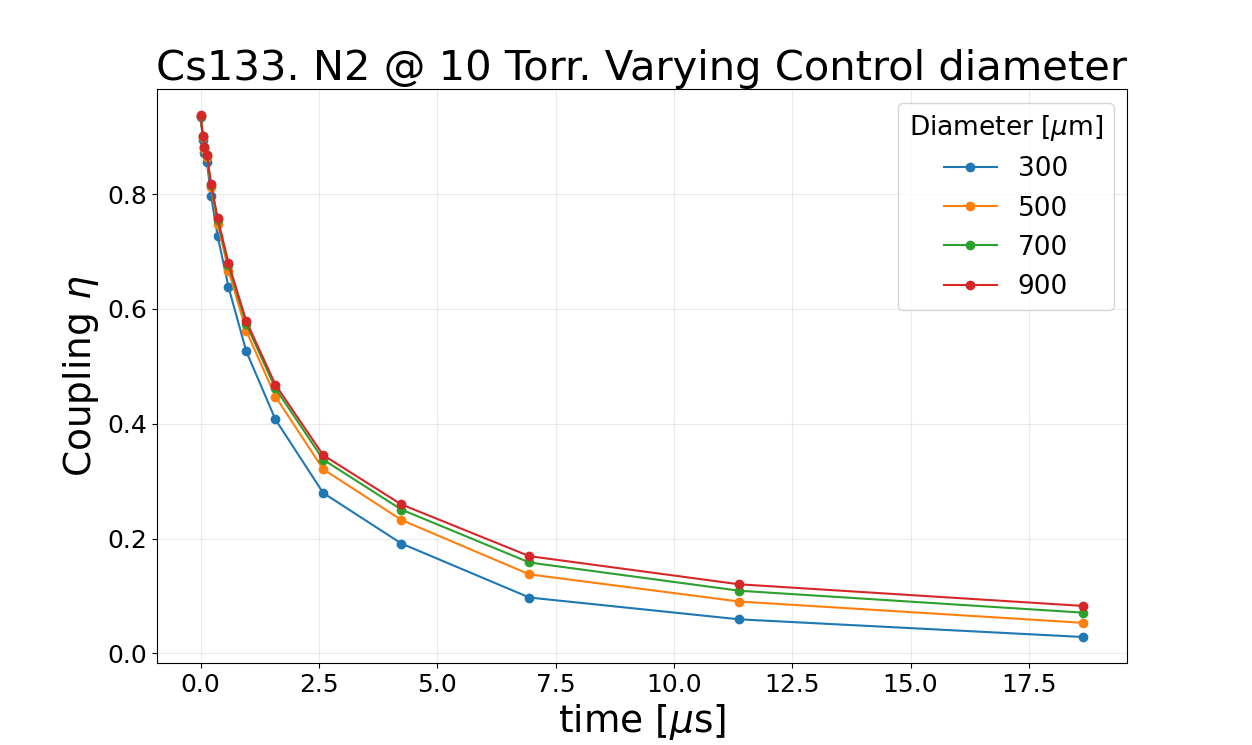
\includegraphics[width=0.78\textwidth]{Figures/beam_size_scan_coupling_decay.jpeg}
    \caption{Normalized fibre-coupled retrieval for different magnetic-field gradients. A spatially varying ground-state splitting causes different parts of the ensemble to accumulate different phases, thereby reducing constructive retrieval into the target optical mode.}
    \label{fig:magnetic_gradient_scan}
\end{figure}



\subsection{Control--Signal Beam Angle}
\label{sec:results_beam_angle}

A non-zero angle between the signal and control beams can assist the spatial separation and filtering of the weak retrieved signal from the strong control field. This experimental advantage is accompanied by a change in the spin-wave wave vector,
\begin{equation}
    \Delta\mathbf{k}
    =
    \mathbf{k}_{\mathrm{sig}}
    -
    \mathbf{k}_{\mathrm{ctrl}}.
\end{equation}
Increasing the angle increases $|\Delta\mathbf{k}|$ and reduces the corresponding spin-wave wavelength. Atomic motion then produces a larger phase change for a given displacement,
\begin{equation}
    \delta\phi_j(t)
    =
    \Delta\mathbf{k}\cdot
    \left[
        \mathbf{r}_j(t)-\mathbf{r}_j(0)
    \right].
\end{equation}

The collective readout therefore becomes more sensitive to atomic motion as the angle is increased. The beam angle must consequently be selected by balancing the improved spatial filtering against the resulting increase in motion-induced spin-wave dephasing.
\section{Magnetic-Field Homogeneity}
\label{sec:results_magnetic_gradient}

In addition to motion-induced loss of spatial overlap, collective retrieval can be reduced by magnetic-field inhomogeneity. The relevant quantity is the differential Zeeman shift of the two ground states forming the stored coherence,
\begin{equation}
\Delta\omega_{sg}(B)
=
\frac{E_s(B)-E_g(B)}{\hbar}.
\end{equation}
For sufficiently weak fields, this shift can be approximated as
\begin{equation}
\Delta\omega_{sg}(B)
\simeq
\Delta\omega_{sg}^{(0)}
+
\beta B,
\qquad
\beta
=
\frac{\mu_{\mathrm B}}{\hbar}
\left(
g_{F_s}m_{F_s}
-
g_{F_g}m_{F_g}
\right),
\label{eq:results_zeeman_sensitivity}
\end{equation}
where $\beta$ denotes the differential magnetic sensitivity of the selected ground-state coherence. A spatially uniform magnetic field produces the same phase shift for all atoms. For a single selected coherence, this common phase changes the phase of the retrieved optical field but does not reduce its intensity. Dephasing is produced only by spatial variations of the field, since different atoms then accumulate different phases before retrieval.

The origin and structure of these inhomogeneities differ between the two platforms. In a warm-vapour cell, external magnetic fields can be strongly attenuated by $\mu$-metal shielding, although residual gradients may remain because of shield apertures, remanent magnetization, nearby magnetic materials, heater currents, and imperfect compensation. Laboratory measurements indicate residual gradients of order $\SI{10}{\nano\tesla\per\centi\metre}$. In a cold-atom experiment, the quadrupole field used for the magneto-optical trap must be switched off before the memory sequence. The residual field is then determined by coil-current decay, eddy-current transients, compensation errors, and spatial curvature. Its evolution can be both time dependent and non-linear across the expanding cloud, which makes a realistic field model strongly dependent on the specific coil geometry, switching electronics, and surrounding conducting structures. The smaller initial size of the cold ensemble reduces the field variation sampled at short times, but ballistic expansion increases the sampled volume during longer storage intervals and may expose higher-order spatial variations. Because these details are experiment specific and are not constrained by the present model, the numerical study is restricted to a static linear magnetic-field gradient in the warm-vapour system. This simpler case isolates the basic phase-scrambling mechanism and allows the required field homogeneity to be assessed without introducing poorly determined cold-atom transients.
The magnetic phase accumulated by atom $j$ is calculated along its trajectory as
\begin{equation}
\delta\phi_j(t)
=
\int_0^t
\left[
\Delta\omega_{sg}
\left(
\mathbf r_j(t')
\right)
-
\Delta\omega_{\mathrm{ref}}
\right]
dt',
\label{eq:results_magnetic_phase}
\end{equation}
where $\Delta\omega_{\mathrm{ref}}$ removes the common frequency shift. In the present simulation, the magnetic field is approximated by a linear axial gradient,
\begin{equation}
B_z(z)
=
B_0+G_z z,
\qquad
G_z
=
\frac{\partial B_z}{\partial z}.
\label{eq:results_linear_magnetic_gradient}
\end{equation}
The corresponding relative phase is therefore
\begin{equation}
\delta\phi_j(t)
=
\beta G_z
\int_0^t
\left[
z_j(t')-z_{\mathrm{ref}}
\right]
dt'.
\label{eq:results_linear_gradient_phase}
\end{equation}
This model assumes a fixed quantization axis and isolates dephasing caused by the longitudinal field component. Transverse-field-induced state mixing and time-dependent magnetic noise are not included.
The magnetic-gradient scan is performed for a warm $^{133}\mathrm{Cs}$ ensemble contained in a cylindrical cell of length $\SI{75}{\milli\metre}$ and diameter $\SI{4}{\milli\metre}$. The cell contains $\SI{10}{\Torr}$ of $\mathrm{N_2}$ buffer gas and is operated at $\SI{75}{\degreeCelsius}$. The signal and control beams have FWHM diameters of $\SI{120}{\micro\metre}$ and $\SI{300}{\micro\metre}$, respectively. The stored coherence is formed between
\begin{equation}
    \ket{g}
    =
    \ket{F=3,m_F=+3},
    \qquad
    \ket{s}
    =
    \ket{F=4,m_F=+4}.
\end{equation}
This coherence is linearly sensitive to magnetic fields, with a weak-field sensitivity of approximately
    $\frac{\beta}{2\pi}
    \simeq
    \SI{2.45}{\hertz\per\nano\tesla}.
$
Axial gradients between $\SI{0}{\nano\tesla\per\centi\metre}$ and $\SI{1e3}{\nano\tesla\per\centi\metre}$ are applied along the propagation direction. Since the cell is considerably longer than it is wide, an axial gradient produces the largest field variation across the ensemble for a given gradient magnitude and therefore provides a conservative test case.

\begin{figure}[htbp]
    \centering
    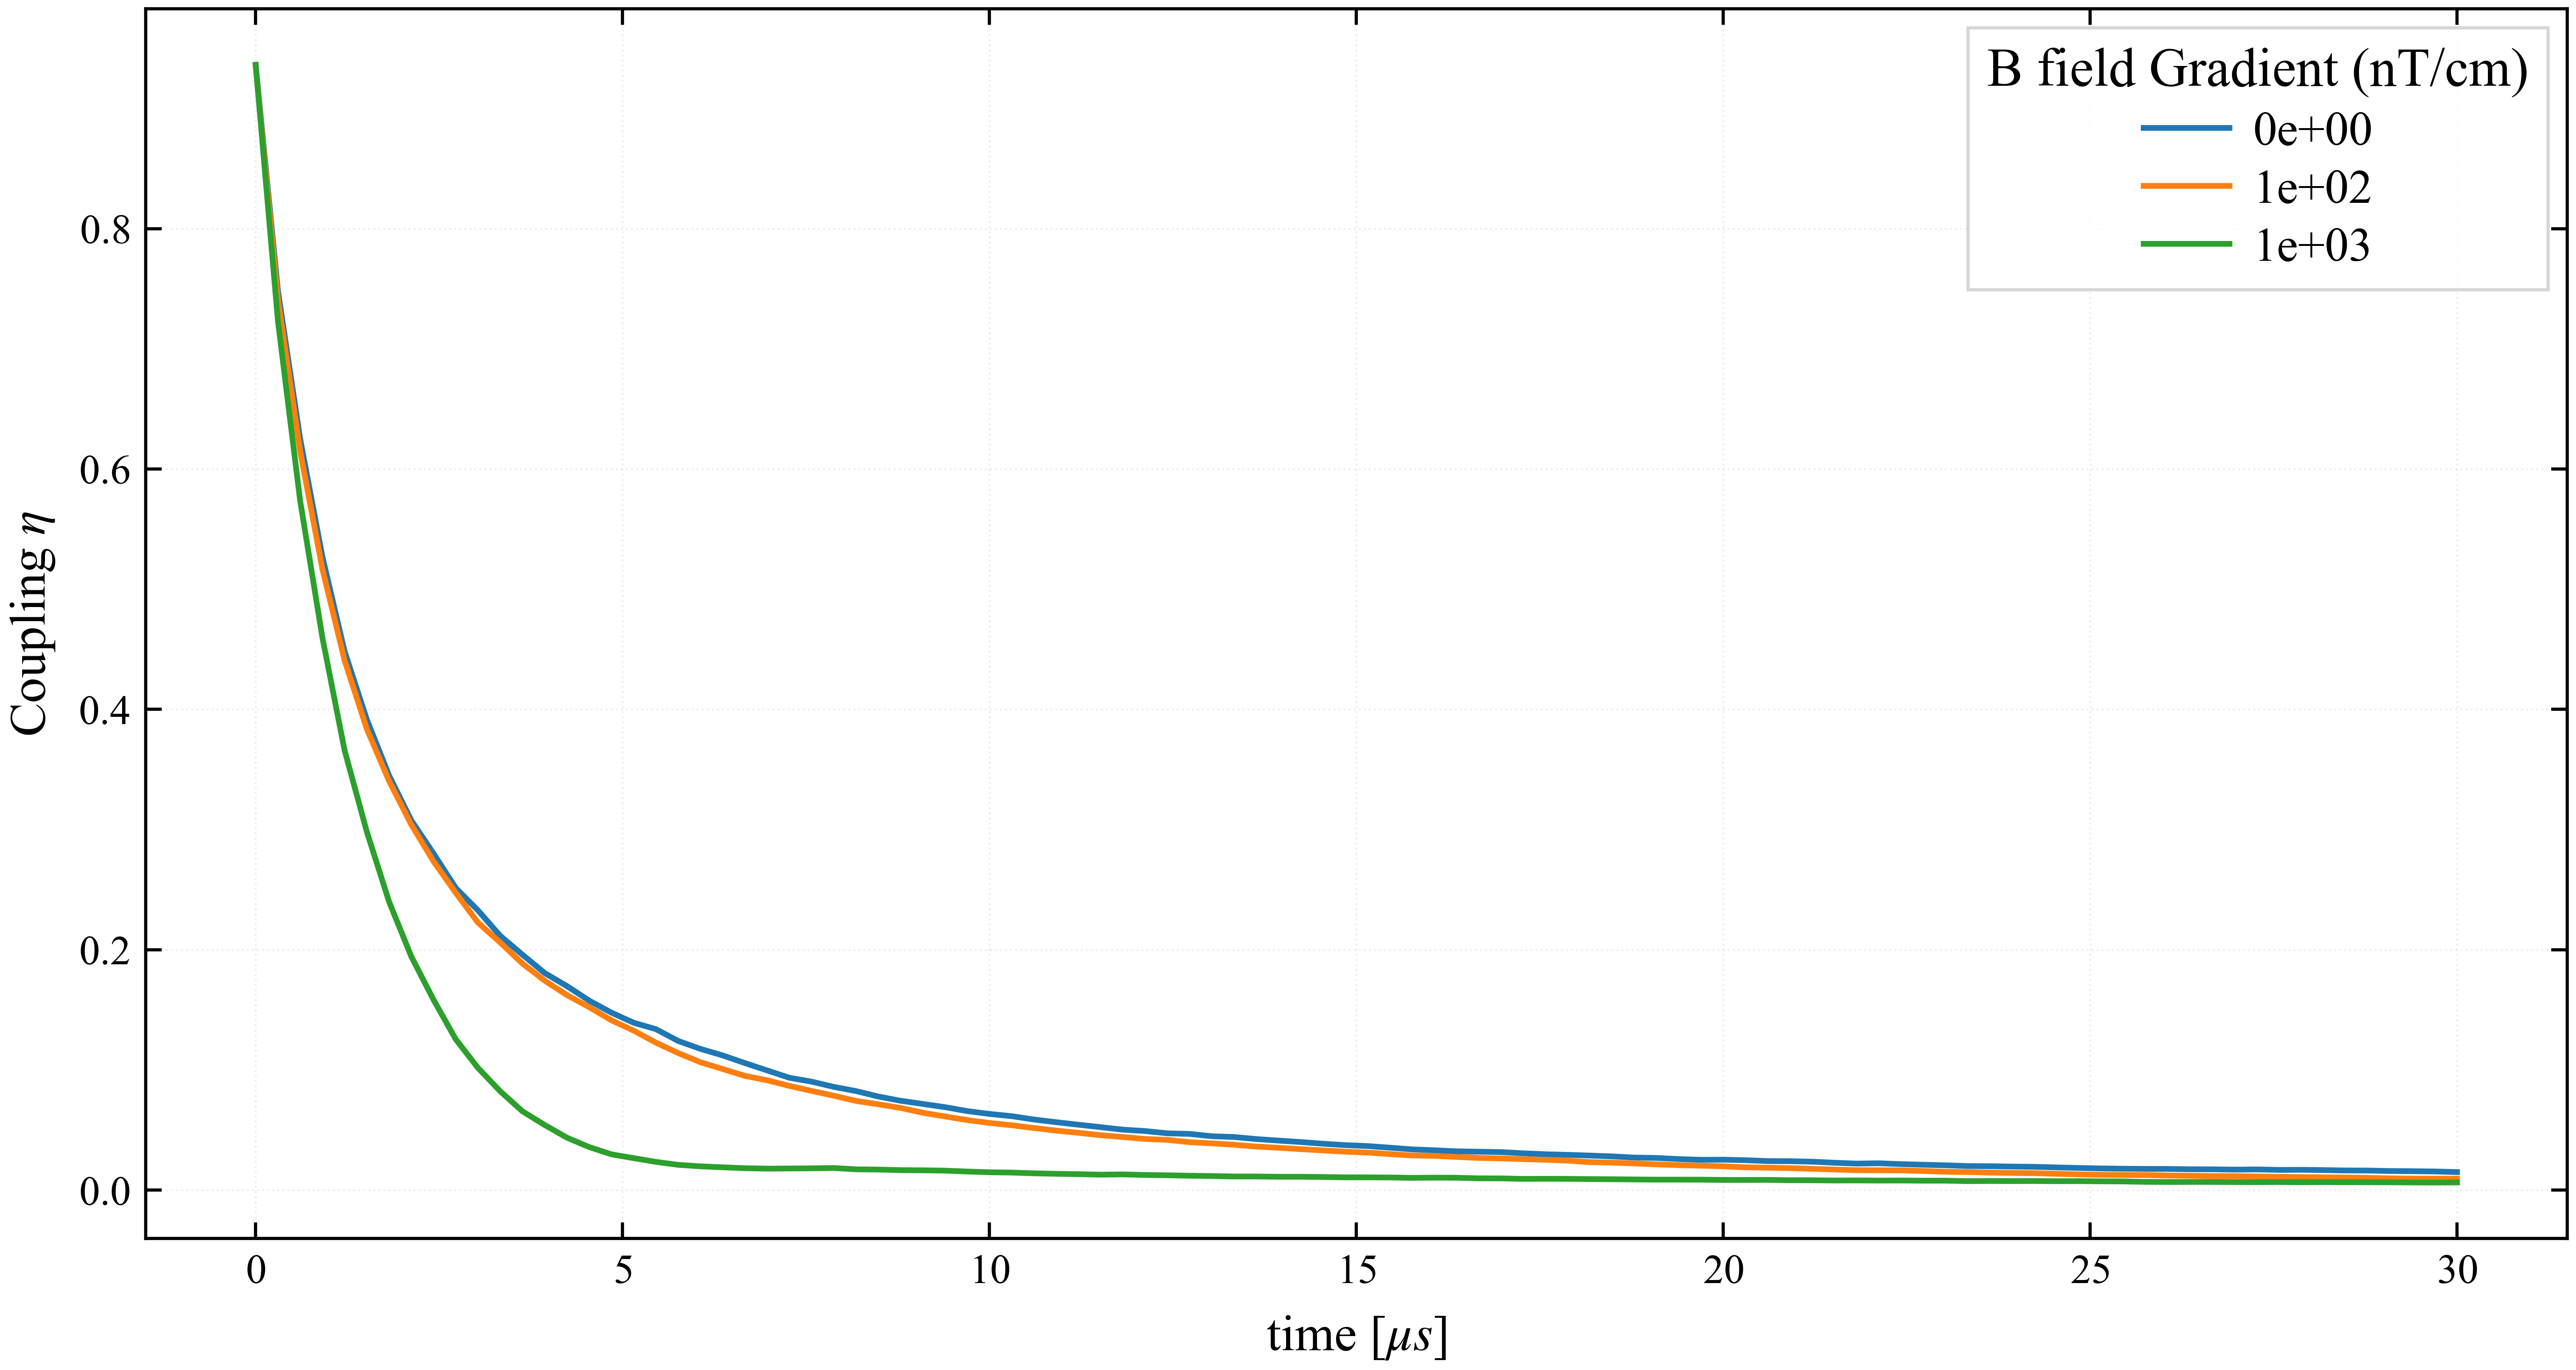
\includegraphics[width=0.72\textwidth]{Figures/magnetic_gradient_scan.png}
    \caption{Normalized fibre-coupled retrieval for different axial magnetic-field gradients $G_z=\partial B_z/\partial z$. The simulation considers a $^{133}\mathrm{Cs}$ cell of length $\SI{75}{\milli\metre}$ and diameter $\SI{4}{\milli\metre}$, operated at $\SI{75}{\degreeCelsius}$ with $\SI{10}{\Torr}$ of $\mathrm{N_2}$ buffer gas. The signal and control beams have FWHM diameters of $\SI{120}{\micro\metre}$ and $\SI{300}{\micro\metre}$, respectively.}
    \label{fig:magnetic_gradient_scan}
\end{figure}

Figure~\ref{fig:magnetic_gradient_scan} shows that the simulated retrieval remains close to the zero-gradient result for gradients up to approximately $\SI{1e2}{\nano\tesla\per\centi\metre}$ over the considered time interval. At larger gradients, the accumulated phase spread becomes appreciable and the fibre-coupled retrieval decays more rapidly. The gradient tolerance depends on the magnetic sensitivity of the selected coherence, the ensemble dimensions, the atomic trajectories, and the retrieval time.

The onset of magnetic dephasing in the simulation occurs at gradients approximately three orders of magnitude larger than those measured in the laboratory. Under the present warm-vapour conditions, magnetic-field inhomogeneity is therefore not expected to be the dominant limitation on the retrieved mode. Nevertheless, magnetic shielding and active field compensation remain necessary because this dephasing mechanism cannot be mitigated by increasing the optical beam size. An atom may remain within the illuminated region while ceasing to contribute constructively once its internal phase is no longer aligned with the remainder of the ensemble. Magnetic homogeneity must therefore be controlled independently of the spatial-overlap losses considered in the preceding sections.

%\section{Cell Dimensions and the Wall-Collision Regime}
\label{sec:results_compact_cell_geometry}

The dimensions of a vapour cell are fixed once the cell has been fabricated and must therefore be selected before the optical system is assembled. They determine the available optical path length, the surface-to-volume ratio of the vapour, and the distance that an atom can diffuse before reaching a boundary. These effects cannot be considered independently of the optical beam dimensions. A cell that is large compared with the signal and control modes behaves differently from a compact cell in which the optical fields occupy a substantial fraction of the available transverse area.

The physical connection between the cell geometry and the retrieved field follows from the collective spin-wave description in Sec.~\ref{sec:collective_spin_wave_storage}. The stored coherence between the ground states $\ket{g}$ and $\ket{s}$ has the spatial form given in Eq.~\eqref{eq:continuous_spin_wave_initial}. During storage, each atom moves away from the position at which it initially contributed to this mode. Its contribution to the readout is consequently modified through the spatial weight $W_j(t)$ in Eq.~\eqref{eq:time_dependent_weight} and through the phase entering the coherent sum in Eq.~\eqref{eq:array_factor_general}. An atom may therefore retain its internal $\ket{g}$--$\ket{s}$ coherence while no longer contributing efficiently to the fibre-coupled field.

\subsection{Transverse Cell Size and Diffusive Transport Regimes}
\label{subsec:transverse_cell_size}

The reference vapour cell is much wider than the optical interaction region. In this limit, the signal and control beams define a localized region near the cell axis, while the radial wall remains far from the atoms that initially carry most of the spin-wave amplitude. Atomic diffusion first moves these atoms out of the high-overlap optical region. Their contribution to retrieval decreases because the readout weight $u_{\mathrm{read}}(\mathbf{r}_j(t))$ in Eq.~\eqref{eq:time_dependent_weight} becomes small, even though the atoms may not yet have encountered the cell boundary. This regime may therefore be described as \emph{mode limited}: the relevant loss is primarily the loss of spatial overlap with the optical mode.

The transverse displacement expected from the diffusion model can be estimated from Eq.~\eqref{eq:diffusion_msd}. For isotropic diffusion, the root-mean-square displacement in the plane perpendicular to the optical axis is~\cite{MonteCarloNotes}
\begin{equation}
\ell_{\perp}(t)
=
\sqrt{
\left\langle
\Delta x^2+\Delta y^2
\right\rangle
}
=
\sqrt{4Dt},
\label{eq:results_transverse_diffusion_length}
\end{equation}
where $D$ is the diffusion coefficient and $\ell_{\perp}(t)$ is the characteristic transverse distance explored during the storage time $t$. If $\ell_{\mathrm{wall}}$ denotes a representative distance between the initially occupied spin-wave region and the cell wall, the corresponding wall-encounter timescale is approximately
\begin{equation}
\tau_{\mathrm{wall},\perp}
\sim
\frac{\ell_{\mathrm{wall}}^2}{4D}.
\label{eq:results_transverse_wall_time}
\end{equation}
This expression is an order-of-magnitude estimate rather than a fit to the simulated decay. Its purpose is to identify whether the boundary is expected to be reached during the relevant storage interval.

A different regime is entered when the cell diameter is reduced while the optical beam sizes are maintained. The compact geometry considered here has an internal diameter of $\SI{1}{\milli\metre}$ and a length of $\SI{10}{\milli\metre}$. The control and signal intensity profiles have FWHM diameters of approximately $\SI{0.8}{\milli\metre}$ and $\SI{0.3}{\milli\metre}$, respectively. The control mode therefore extends across a large fraction of the transverse cell aperture. Because a Gaussian field does not have a sharp edge, the FWHM contour should not be interpreted as the complete optical extent of the beam. A non-negligible control-field amplitude is present beyond this contour and approaches the radial wall.

Under these conditions, atoms that diffuse away from the initially populated signal mode can remain within the broader control or readout field while approaching the boundary. The timescale for leaving the optical mode can then become comparable to the timescale for reaching the wall. Spatial escape and wall interaction can no longer be separated into independent stages. The system instead operates in a mixed transport regime in which atoms may leave the strongest part of the mode, collide with the surface, and later return to the illuminated region.

The cell radius is $\SI{0.5}{\milli\metre}$, whereas the distance from the centre of the cell to either end cap is $\SI{5}{\milli\metre}$. For atoms initially located near the centre, the characteristic axial distance to an end cap is therefore approximately ten times larger than the radial distance to the cylindrical wall. Since diffusive times scale with the square of the travelled distance, radial wall encounters are expected to occur approximately two orders of magnitude earlier than end-cap encounters under otherwise identical conditions. The early compact-cell decay is therefore expected to be more sensitive to the internal diameter than to the total cell length.

This distinction is important when a cell is selected experimentally. Reducing the diameter lowers the cell volume and may simplify heating, magnetic shielding, and mechanical integration. It also increases the frequency with which the stored atoms sample the surface. The internal diameter must therefore be chosen with sufficient clearance for the largest optical beam, including the low-intensity wings of the Gaussian profile and the expected alignment tolerance. A diameter that only accommodates the nominal FWHM of the control beam leaves little tolerance for beam displacement, window imperfections, or thermal changes in the optical alignment.

\subsection{Wall Coatings as an Effective Boundary Condition}
\label{sec:results_wall_coatings}

A wall encounter affects the stored excitation through two physically separate processes. The first is mechanical. The atom reaches the cell boundary, interacts with the surface, and eventually returns to the vapour volume. The second concerns its internal state. During the interaction with the surface, the coherence between $\ket{g}$ and $\ket{s}$ may acquire an uncontrolled phase or may be destroyed completely. Mechanical return to the vapour does not therefore guarantee that the atom remains part of the retrievable spin wave.

Atoms that reach a glass surface can remain adsorbed for a finite residence time before returning to the vapour. During this interval, magnetic interactions, electric-field gradients, spin-dependent interactions, and coupling to the surface can perturb the electronic and hyperfine state. The accumulated perturbation varies between wall encounters and can randomize the ground-state coherence carried by the atom~\cite{OP_Happer_1972}. A bare or poorly prepared glass surface can consequently behave as a strongly depolarizing boundary even when the atom is not permanently removed from the vapour.

Anti-relaxation coatings are used to reduce this surface-induced loss. A coating separates the alkali atom from the underlying glass and changes the adsorption dynamics. The probability of preserving the atomic spin depends on the coating material, its surface coverage, molecular ordering, preparation procedure, alkali exposure, and operating temperature~\cite{Aiacoavc_ChiEtAl_2020}. Coating performance is therefore not a universal material constant. A coating characterized at room temperature or before exposure to cesium may not provide the same spin survival under the actual operating conditions of the memory.

\section{section name}%
\label{sec:section name}


The coating material determines the range of $N_{\mathrm{b}}$ that can realistically be expected and the temperature over which this performance can be maintained. This trade-off is particularly important for a compact vapour cell. Increasing the temperature raises the atomic density and can provide the optical depth required for efficient EIT storage, but the selected coating must remain effective at that temperature. A coating with a very large $N_{\mathrm{b}}$ at room temperature may therefore be less suitable than a more thermally stable coating with a smaller collision-survival number.

The principal coating families considered for alkali-vapour cells are compared in Table~\ref{tab:coating_comparison}. The values should be regarded as representative ranges reported in the coating literature rather than as fixed material constants~\cite{Aiacoavc_ChiEtAl_2020}. The measured $N_{\mathrm{b}}$ also depends on the alkali species, cell geometry, fabrication procedure, and method used to extract the wall-relaxation rate.

\begin{table}[htbp]
    \centering
    \label{tab:coating_comparison}
    \begin{tabular}{lcc}
        \hline
        \textbf{Compound} & \textbf{$N_{\mathrm{b}}$} & \textbf{Temperature} \\
        \hline
        Alpha-olefin fraction C20--24 & $\sim 10^{6}$ & $\SI{33}{\degreeCelsius}$ \\
            1-Nonadecene & $\sim 10^6$  & $\SIrange{20}{60}{\degreeCelsius}$ \\
        Tetracontane, $\mathrm{C}_{40}\mathrm{H}_{82}$ & $10^{3}$--$10^{4}$ & $\SIrange{60}{80}{\degreeCelsius}$ \\
        Octadecyltrichlorosilane (OTS) & $\sim 2100$ & $>\SI{170}{\degreeCelsius}$ \\
        \hline
    \end{tabular}
    \caption{Representative anti-relaxation coatings for alkali-vapour cells~\cite{Aiacoavc_ChiEtAl_2020}.}
\end{table}

Straight-chain alkane coatings, of which paraffin is the conventional example, form physically adsorbed films on the inner glass surface. They can preserve the atomic polarization over approximately $10^{4}$ wall encounters, which represents a substantial improvement over an uncoated surface~\cite{Aiacoavc_ChiEtAl_2020}. Their main limitation is thermal stability. Paraffin softens or melts as the temperature is increased and generally ceases to provide reliable anti-relaxation behaviour above approximately $\SI{80}{\degreeCelsius}$. This restricts its use when a high atomic density must be obtained by strongly heating the cell.

Alkene coatings are also physically adsorbed films, but contain unsaturated C=C bonds. High-quality alkene coatings have produced exceptionally long spin-relaxation times, corresponding in the best reported room-temperature cells to collision numbers approaching $N_{\mathrm{b}}\sim10^{6}$~\cite{Aiacoavc_ChiEtAl_2020}. Such values are well above the range for which the simulated curves become insensitive to further increases in $N_{\mathrm{b}}$. From the perspective of the present model, an alkene coating with this performance would therefore approximate a coherence-preserving boundary over the simulated storage interval. Its experimental disadvantage is that the coating remains subject to the temperature limitations associated with physically adsorbed organic films.

Organochlorosilanes, particularly octadecyltrichlorosilane, provide a different compromise. The silane head group forms chemical bonds with the glass surface, producing a more strongly anchored coating. OTS-coated cells have commonly been reported to preserve polarization over several hundred wall encounters, with the best cells reaching approximately $2\times10^{3}$ encounters~\cite{Aiacoavc_ChiEtAl_2020}. Although this is lower than the best alkene performance, OTS can remain effective at temperatures close to $\SI{160}{\degreeCelsius}$. Degradation has been observed during extended operation near $\SI{170}{\degreeCelsius}$. OTS is therefore relevant when the atomic density required by the experiment cannot be reached within the temperature range tolerated by paraffin or alkene coatings.

For the compact-cell simulations, the coating families in Table~\ref{tab:coating_comparison} provide a physical interpretation of the scanned values of $N_{\mathrm{b}}$. Values around $N_{\mathrm{b}}\sim10^{2}$ represent a modest anti-relaxation coating, while $N_{\mathrm{b}}\sim10^{3}$ is representative of a high-quality thermally robust OTS cell. Values near $N_{\mathrm{b}}\sim10^{4}$ correspond to established paraffin performance, whereas $N_{\mathrm{b}}\gtrsim10^{5}$ represents the exceptionally high survival reported for optimized alkene coatings. The numerical scan therefore covers coating regimes that are experimentally plausible, while also extending to the idealized limit in which wall-induced depolarization becomes negligible.


\section{===}

The microscopic interaction between a particular coating and the atomic state is not resolved in the simulation. It is represented by the effective parameter $N_{\mathrm{b}}$, defined as the mean number of wall encounters that can occur before the ground-state coherence is lost. Following the phenomenological description of repeated wall relaxation~\cite{OP_Happer_1972,Aiacoavc_ChiEtAl_2020}, the survival probability associated with one collision is written as
\begin{equation}
p_{\mathrm{b}}
=
1-\frac{1}{N_{\mathrm{b}}},
\label{eq:results_single_bounce_survival}
\end{equation}
where $p_{\mathrm{b}}$ is the probability that the coherence survives a single wall encounter. If atom $j$ has undergone $n_j(t)$ wall encounters by time $t$, its mean surviving coherence weight is given by Eq.~\eqref{eq:wall_survival_factor},
\begin{equation*}
\eta_j(t)
=
\left(
1-\frac{1}{N_{\mathrm{b}}}
\right)^{n_j(t)}.
\end{equation*}
The limiting case $N_{\mathrm{b}}=1$ represents a fully depolarizing wall, for which the first encounter removes the atom from the coherent spin-wave sum. In the limit $N_{\mathrm{b}}\rightarrow\infty$, wall-induced relaxation is neglected and the coherence is preserved through repeated encounters.

The factor $\eta_j(t)$ enters the time-dependent atomic weight in Eq.~\eqref{eq:time_dependent_weight}. A wall collision therefore does not reduce the retrieved signal as an independent intensity loss applied after the field has been calculated. Instead, it reduces the amplitude contributed by the affected atom before the coherent sum is taken. This distinction is required because the fibre-coupled power is obtained from the squared modulus of the collective amplitude, as shown in Eqs.~\eqref{eq:array_factor_general} and~\eqref{eq:fibre_power}. Removing one coherent contribution changes the interference between that atom and the remainder of the ensemble.

Several classes of anti-relaxation coatings have been studied for alkali-vapour cells. Alkane and alkene coatings can preserve spin polarization over many wall encounters, but their performance may deteriorate at elevated temperatures. Chemically bonded organosilane coatings generally provide greater thermal robustness, although the number of coherence-preserving encounters can be lower than for the best low-temperature hydrocarbon coatings~\cite{Aiacoavc_ChiEtAl_2020}. The most appropriate coating for a compact memory is therefore not necessarily the material with the largest value of $N_{\mathrm{b}}$ reported under any condition. It is the coating that retains an adequate $N_{\mathrm{b}}$ at the temperature required to obtain the desired cesium density and optical depth.

\begin{figure}[htbp]
\centering
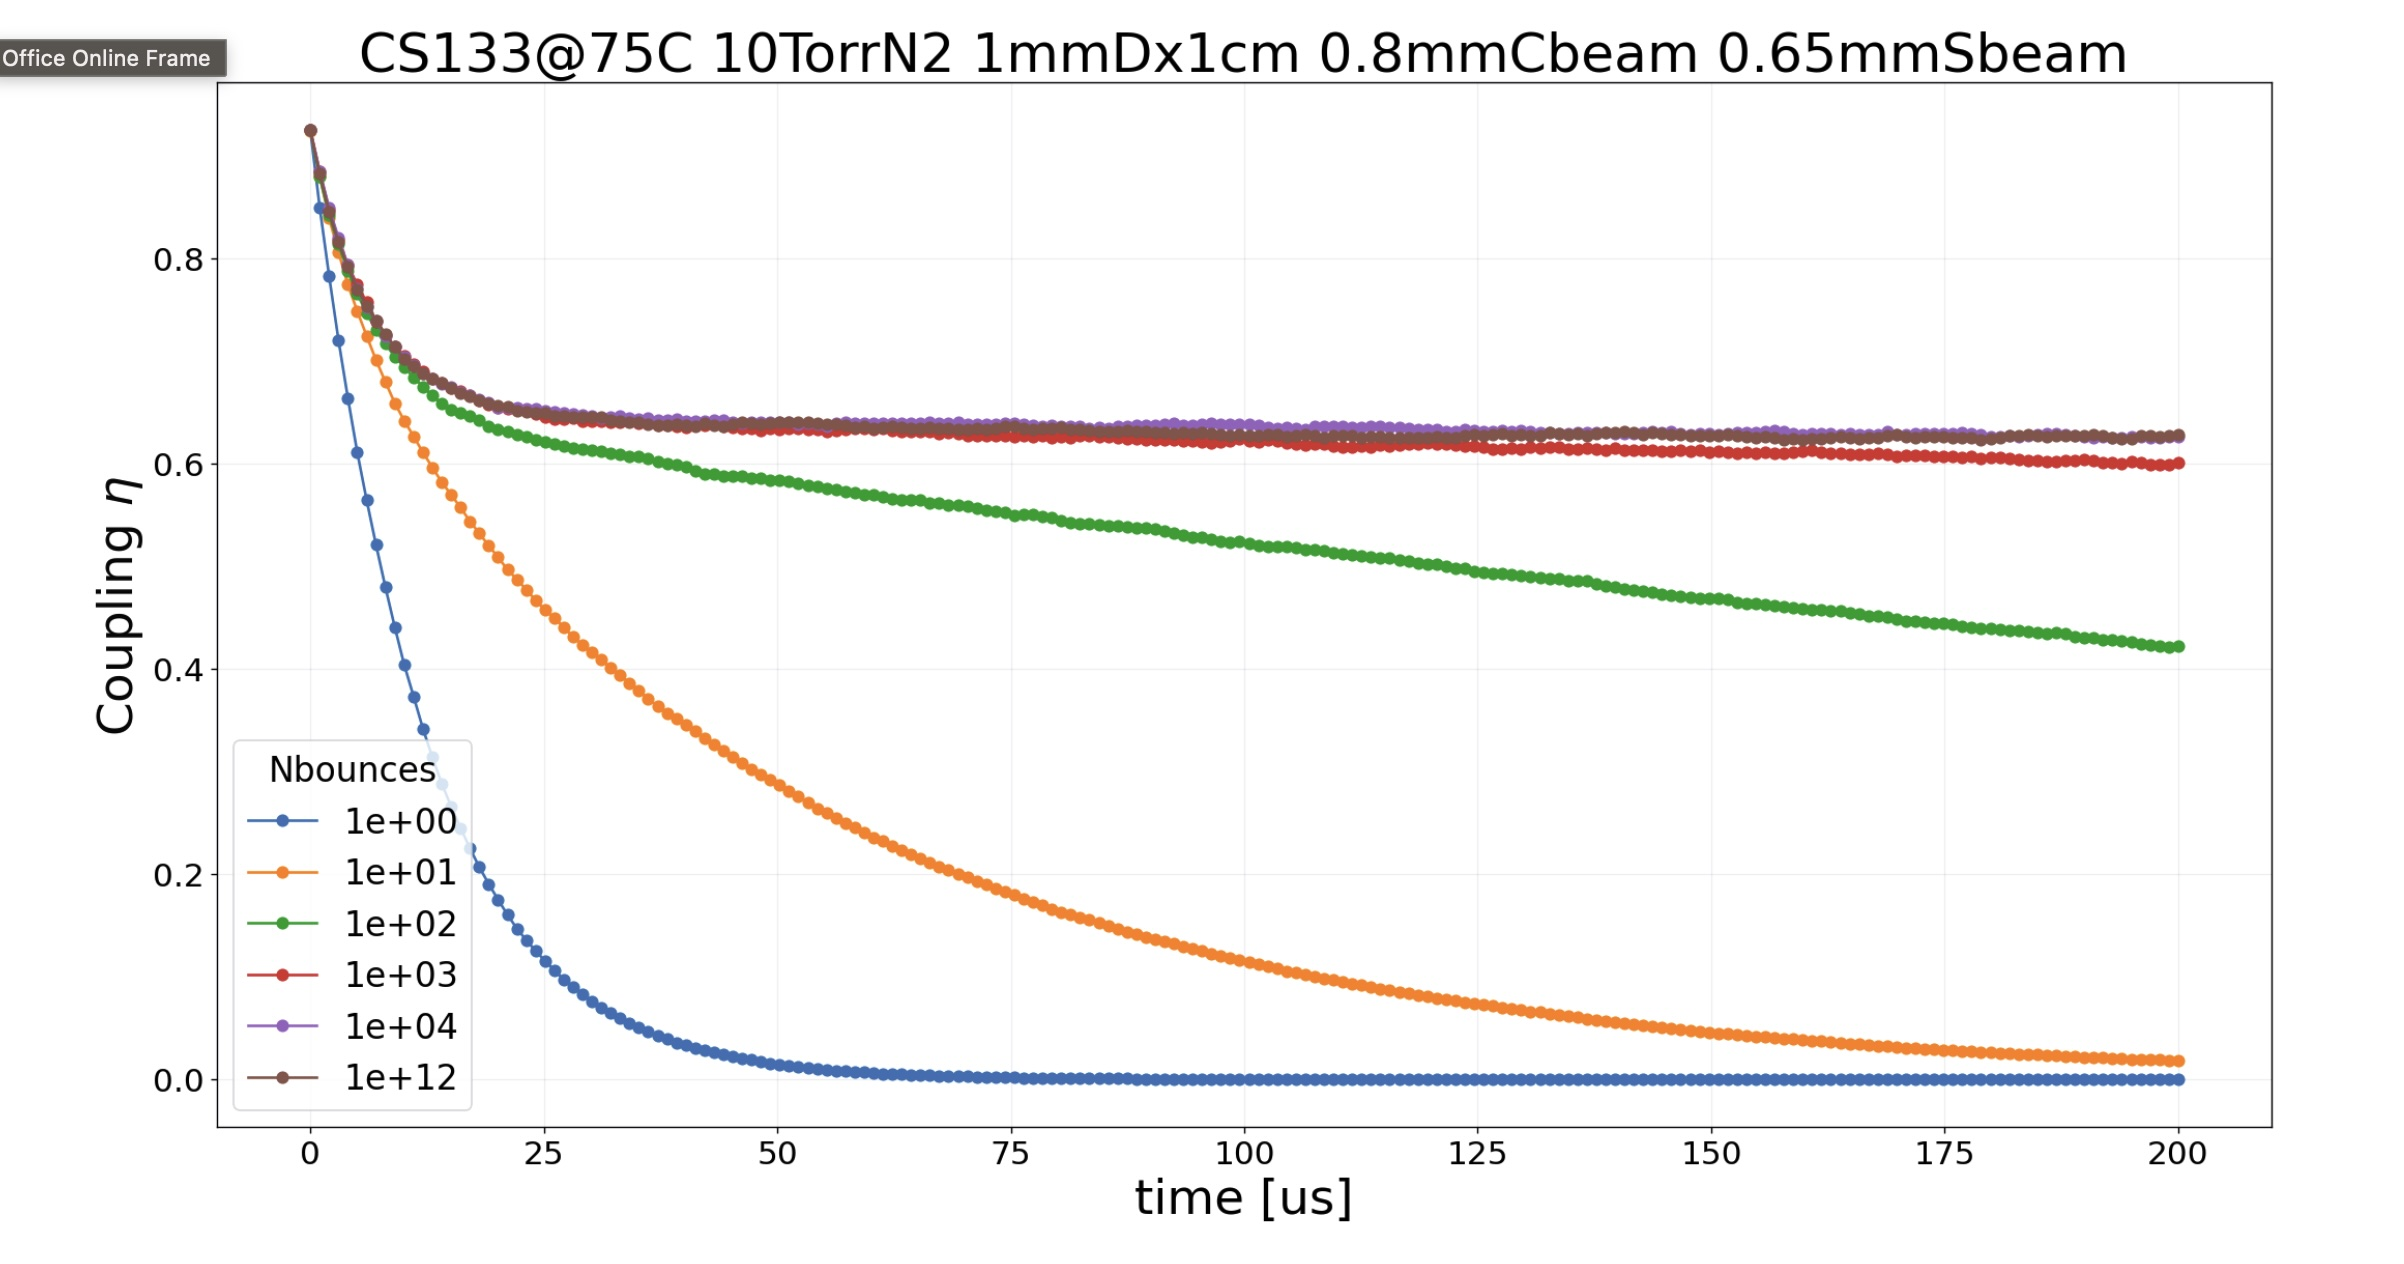
\includegraphics[width=0.72\textwidth]{Figures/coating_bounce_scan.jpeg}
\caption{Normalized fibre-coupled retrieval in the compact cell for different values of the mean coherence-preserving wall-collision number $N_{\mathrm{b}}$. The influence of the coating is strongest when wall-induced relaxation removes a substantial fraction of the atomic contributions from the coherent readout.}
\label{fig:coating_bounce_scan}
\end{figure}

The calculated coating dependence is shown in Fig.~\ref{fig:coating_bounce_scan}. At low $N_{\mathrm{b}}$, each encounter has an appreciable probability of destroying the $\ket{g}$--$\ket{s}$ coherence. The cylindrical wall then behaves as an absorbing boundary for the collective excitation, even though the simulated atom is mechanically reflected and remains inside the cell. Atoms that reach the wall are progressively removed from the amplitude sum, and the fibre-coupled retrieval decreases as the number of wall encounters grows.

Increasing $N_{\mathrm{b}}$ allows a larger fraction of the atoms to remain coherent after reaching the boundary. These atoms may subsequently diffuse back towards the optical axis and recover a non-negligible readout weight. The improvement is therefore most visible at storage times for which a significant part of the ensemble has already sampled the wall. The early-time behaviour can remain comparatively insensitive to the coating because many of the atoms have not yet reached the boundary.

The curves approach one another when $N_{\mathrm{b}}$ becomes sufficiently large. In this regime, the expected survival factor remains close to unity for the number of collisions accumulated during the simulated interval. Wall-induced depolarization is no longer the dominant source of retrieval loss. The remaining decay is then determined mainly by the spatial factor $u_{\mathrm{read}}(\mathbf{r}_j(t))$, motion away from the initially prepared spin-wave envelope, and any loss of collective phase alignment. Improving the coating beyond this point cannot recover atoms whose internal coherence survives but whose spatial contribution no longer matches the fibre mode.

A long tail or plateau at large $N_{\mathrm{b}}$ must consequently be interpreted with care. It does not demonstrate an indefinitely preserved memory. In a finite reflecting volume, atoms can leave the strongly weighted optical region and later return to it. When wall survival is high, these returning atoms can again contribute to the simulated coherent field. Such behaviour represents finite-volume diffusion and recurrence within the assumed boundary conditions. Additional experimental relaxation mechanisms, including residual magnetic gradients, spin-exchange collisions, coating inhomogeneity, and imperfect control-field coverage, would reduce this contribution in a physical cell~\cite{OP_Happer_1972,Apgteitiav_FinkelsteinEtAl_2023}.

For cell procurement, the coating should therefore be specified together with the intended operating temperature and alkali species. A quoted coating name alone is insufficient. The experimentally relevant information is the measured ground-state relaxation time or effective collision number after alkali exposure, under the temperature conditions expected during operation. The coating of the cylindrical wall, end caps, windows, and any stem connected to the vapour reservoir must also be considered, since atoms can sample each of these surfaces during long storage intervals.

\subsection{Cell Length Relative to the Spin-Wave Wavelength}
\label{sec:results_cell_length_spin_wave}

The effect of the cell length is governed by its relation to the axial spin-wave wavelength,
\begin{equation}
    \lambda_{\mathrm{SW},z}
    =
    \frac{2\pi}{|\Delta k_z|},
    \label{eq:results_axial_spin_wave_wavelength}
\end{equation}
where $\Delta k_z$ is the axial component of the spin-wave wave vector. The presence of several spin-wave periods within the cell does not by itself reduce retrieval, since the phase-matched readout addresses the corresponding collective mode. Dephasing arises when atomic motion changes the phase carried by each atom.

An axial displacement $\Delta z_j(t)=z_j(t)-z_j(0)$ produces the phase change
\begin{equation}
    \delta\phi_{j,z}(t)
    =
    \Delta k_z\Delta z_j(t)
    =
    \frac{2\pi\Delta z_j(t)}
         {\lambda_{\mathrm{SW},z}}.
    \label{eq:results_axial_motion_phase}
\end{equation}
Different atomic displacements therefore produce different phases, reducing the constructive interference in the coherent sum of Eq.~\eqref{eq:array_factor_general}.

In a short cell, the axial displacement is restricted to a range smaller than the spin-wave period. When $L\ll\lambda_{\mathrm{SW},z}$, the accessible phase spread remains smaller than $2\pi$, and the atomic contributions cannot become completely dephased. A residual coherent contribution consequently remains, producing the long-time plateau observed in the retrieval.

As the cell length becomes comparable to or larger than $\lambda_{\mathrm{SW},z}$, atoms can explore a broader part of the spin-wave phase pattern. Their phases then span a larger interval and cancel more completely. The reduction of the plateau with increasing $L$ therefore results from the larger range of motion-induced dephasing allowed by the cell geometry.

%%\subsection{Wall coatings as an effective boundary condition}
\label{subsec:wall_coatings}

%The previous sections considered the loss of spin-wave overlap due to atomic motion inside the optical interaction region. This description is sufficient when the optical beams occupy only a small fraction of the transverse cell area, because atoms can diffuse out of the mode before the cell boundary becomes the dominant limitation. In the compact geometry considered here, however, the situation changes. The cell diameter is only \(1~\mathrm{mm}\), while the control and signal beams have FWHM diameters of approximately \(0.8~\mathrm{mm}\) and \(0.3~\mathrm{mm}\), respectively. The optical mode therefore occupies a substantial fraction of the cell cross-section. Under these conditions, diffusion no longer occurs in an effectively unbounded transverse volume: atoms that carry part of the stored spin-wave coherence inevitably encounter the cell wall on the timescale relevant for the memory decay. A realistic interpretation of the simulated decay time \(\tau\) must therefore include not only transport through the buffer gas, but also the boundary condition imposed by the cell surface.

%During the residence time on the surface, the atom is exposed to interactions that are absent during free flight. Happer treats this type of relaxation as arising from fluctuating perturbations to the atomic Hamiltonian, which can include magnetic, electric, and spin-dependent interactions at the surface \cite{OP_Happer_1972}. For alkali atoms on uncoated glass, these perturbations are strong enough that wall collisions have historically been treated as highly depolarizing in optical-pumping experiments \cite{OP_Happer_1972}. The atom may therefore return mechanically to the vapor, but its ground-state coherence can be lost during the surface interaction.

The wall interaction must be separated into two conceptually different processes: mechanical reflection and internal-state survival. Mechanical reflection determines whether the atom remains inside the cell after reaching the boundary. Spin survival determines whether the atom still contributes coherently to the collective ground-state excitation after the collision. Happer describes relaxation in optically pumped vapors using the density matrix and treats many relaxation processes as the result of a weak fluctuating perturbation added to the atomic Hamiltonian,
     $
     \hat{H}(t) = \hat{H}_0 + \hat{V}(t),
    \label{eq:weak_fluctuation_hamiltonian}
    $
where \(\hat{H}_0\) is the unperturbed atomic Hamiltonian and \(\hat{V}(t)\) represents a random perturbation that varies from atom to atom and from collision to collision \cite{OP_Happer_1972}. In the case of wall relaxation, this perturbation is not applied continuously during free flight. Instead, it acts primarily when the atom interacts with the cell surface. Thus, an atom may elastically return to the vapor while its electronic or hyperfine coherence has already been randomized.

Upon striking the wall, an atom does not necessarily rebound immediately. It may stick to the surface for a finite dwell time before desorbing back into the vapor \cite{OP_Happer_1972,Aiacoavc_ChiEtAl_2020}. During this residence time, thermal agitation can cause the atom to hop between adsorption sites. Happer gives the average dwell time in the form
\begin{equation}
    \tau_{\mathrm{s}}
    =
    \tau_0
    \exp\!\left(\frac{E_{\mathrm{a}}}{k_{\mathrm{B}}T}\right),
    \label{eq:dwell_time}
\end{equation}
where \(\tau_0\) is a microscopic attempt time, \(E_{\mathrm{a}}\) is the adsorption energy, \(k_{\mathrm{B}}\) is Boltzmann's constant, and \(T\) is the wall temperature \cite{OP_Happer_1972}. While the atom is adsorbed, local magnetic fields, electric-field gradients, spin-orbit interactions, or nuclear spins in the substrate can act as random perturbations \cite{OP_Happer_1972}. These perturbations generate random phase shifts and spin relaxation. For an uncoated glass wall, this interaction is typically strong enough that a wall encounter can be treated, to a good approximation, as a fully depolarizing event for an alkali atom. In the absence of buffer gas, the relaxation time is then closely connected to the average flight time between wall collisions and therefore scales with the characteristic linear dimension of the cell \cite{OP_Happer_1972}. This scaling is precisely why wall effects become increasingly important as the vapor cell is miniaturized.

Anti-relaxation coatings reduce this surface-induced relaxation by separating the alkali atom from the strongly perturbing glass substrate. The coating provides a molecular layer in which the atom can adsorb and desorb with a smaller probability of spin randomization. If the perturbation accumulated during one surface encounter is weak, the spin state is only slightly changed after a single bounce and the atom can survive many wall bounces before losing its polarization. The coating can therefore be characterized by an average number of coherence-preserving collisions, denoted here by \(N_{\text{b}}\). Equivalently, one can describe the coating by a depolarization probability per bounce. This effective description is useful because the full microscopic surface dynamics are complex and material dependent.

Following the classification framework established by Chi et al.~\cite{Aiacoavc_ChiEtAl_2020}, the main coating families for alkali-vapor cells include straight-chain alkanes, alkenes, and organochlorosilanes. Straight-chain alkanes, such as paraffin, form ``wet'' films mainly through physical adsorption on the inner glass surface. These coatings were among the first successful anti-relaxation coatings and can allow alkali atoms to undergo many wall collisions before depolarization, with typical reported values around \(N_{\text{b}}\sim 10^4\). Their chemical structure is dominated by saturated C--C bonds. These bonds have relatively low polarizability and weak adsorption energies, which helps reduce spin-randomizing interactions during wall contact. However, paraffin-based coatings are limited by thermal stability and are generally unsuitable for high-temperature operation.

Alkene coatings are also physically adsorbed films, but they contain unsaturated C=C bonds. These bonds are more polarizable than saturated C--C bonds, and early intuition might suggest that this would be harmful for spin preservation. However, experiments discussed in the coating literature show that C=C bonds are not necessarily strongly depolarizing, and alkene coatings can reach very large bounce numbers, in some cases approaching \(N_{\text{b}}\sim 10^6\) \cite{Aiacoavc_ChiEtAl_2020}. Their main limitation is again temperature stability: their anti-relaxation performance can degrade at temperatures that are relevant for high-density alkali vapors. This makes them attractive from the point of view of spin survival, but less suitable when high optical depth requires elevated cell temperature.

Organochlorosilanes, such as octadecyltrichlorosilane (OTS), represent a different chemical strategy. Instead of forming only a physically adsorbed wet film, these coatings can form chemically bonded dry films. The chlorosilane end groups react with hydroxyl groups on the glass or silicon surface, producing siloxane bonds that anchor the organic layer to the substrate \cite{Aiacoavc_ChiEtAl_2020}. This chemical attachment improves thermal robustness and allows operation at substantially higher temperatures than typical paraffin or alkene coatings. The trade-off is that the spin survival is usually lower, with reported maximum values closer to \(N_{\text{b}}\sim 10^3\) than to the best alkene coatings. Thus, organochlorosilanes are not necessarily the best coatings in terms of bounce number, but they are important for compact warm-vapor memories because they remain usable in temperature regimes where high optical depth becomes accessible.

The coating literature also shows that the anti-relaxation mechanism is not completely settled. For paraffin, models based on adsorption, electron-randomization relaxation, spin-exchange relaxation, and relaxation associated with atoms in stems or reservoirs have been developed. Chi et al. emphasize that surface-science techniques are increasingly used to study coating composition and morphology, including methods such as atomic force microscopy, ellipsometry, X-ray diffraction, and contact-angle measurements \cite{Aiacoavc_ChiEtAl_2020}. These measurements are relevant because coating performance depends not only on the chemical family, but also on thickness, roughness, surface coverage, molecular ordering, adsorption energy, and the interaction between the coating and the alkali atom. For this reason, \(N_{\text{b}}\), atomic dwell time, hyperfine relaxation, and storage time are best understood as effective experimental characterizations of a complicated microscopic surface.

Temperature makes this trade-off central for warm-vapor quantum memories. Increasing the cell temperature raises the alkali vapor pressure and therefore the optical depth \(d\), which is beneficial for storage and retrieval efficiency. At the same time, a higher temperature increases the thermal velocity \(v_{\mathrm{th}}\), modifies the diffusion constant, increases the frequency with which atoms sample the cell boundary, and can degrade or modify the coating itself. Temperature therefore plays two opposite roles. It improves the optical interaction by increasing atomic density, but it can reduce the spin-wave lifetime through faster motion and stronger wall-related relaxation. This creates the central optimization problem for the compact cell: the memory should operate at a temperature high enough to provide sufficient optical depth, but not so high that wall-induced relaxation or coating degradation dominates the decay.

The present simulation does not attempt to resolve the microscopic chemistry of the coated surface. Instead, the coating is represented as an effective stochastic boundary condition. When an atom reaches the cylindrical wall or one of the end caps, its trajectory is reflected according to the chosen kinematic boundary rule. Independently of this mechanical reflection, its spin-wave contribution is multiplied by a survival factor. A simple parametrization is
\begin{equation}
    p_{\mathrm{survive}}
    =
    1 - \frac{1}{N_{\text{b}}},
    \label{eq:survival_probability}
\end{equation}
where \(N_{\text{b}}\) is the average number of wall collisions an atom can undergo before losing its coherence. This parameter condenses the surface material, adsorption dynamics, and microscopic relaxation mechanisms into a single quantity that can be varied numerically.

This abstraction also clarifies how coatings change the interpretation of the simulation results. In the low-survival limit, corresponding to bare glass or a poor coating, wall collisions act as an absorbing boundary for the spin wave. In that regime, increasing the buffer-gas pressure can improve the memory lifetime by slowing diffusion and reducing the probability that atoms reach the wall during the storage time. In the high-survival limit, corresponding to an effective anti-relaxation coating, atoms can collide with the wall and later re-enter the optical mode while still carrying coherence. This can produce long non-exponential tails in the retrieved coupling, because part of the ensemble temporarily leaves the high-overlap region and later returns.

The simulations therefore probe a regime that is not captured by the two simplest analytical limits. The limit \(N_{\text{b}}=0\) corresponds to immediate spin destruction at the wall, while \(N_{\text{b}}\rightarrow\infty\) corresponds to perfect coherence preservation. Real coated compact cells lie between these extremes. In particular, when the cell radius, beam waist, and diffusion length are comparable, the retrieval decay depends on the combined effect of beam geometry, buffer gas, temperature, and wall survival. The numerical results show that increasing \(N_{\text{b}}\) strongly improves the decay for poor coatings, but that the curves tend to converge once \(N_{\text{b}}\sim 10^3\text{ to }10^4\). Above this range, wall-induced depolarization is no longer the dominant loss channel. The remaining reduction of coupling is then mainly set by diffusion out of the signal and control mode volume, finite cell geometry, and the spatial overlap of the spin wave with the readout mode. This is why the coating model is essential for interpreting the simulated \(\tau\)-versus-temperature trends in compact vapor cells.

%%
%%\input{compact_newSystem.tex}
%
%\addcontentsline{toc}{chapter}{References}
%\printbibliography
%\appendix 
%\chapter{Anti-Relaxation Coatings for Alkali-Vapour Cell}
\label{app:anti_relaxation_coatings}
Anti-relaxation coatings are used to reduce the loss of atomic polarization and ground-state coherence caused by collisions with the inner surface of an alkali-vapour cell. Their function is not to prevent atoms from reaching the wall, but to modify the atom--surface interaction so that a wall encounter produces a smaller perturbation of the internal state. The coating therefore acts as an effective boundary material between the alkali vapour and the underlying glass substrate. Its performance depends on both the chemical structure of the coating and the microscopic properties of the deposited film.

Following the classification framework established by Chi et al.~\cite{Aiacoavc_ChiEtAl_2020}, the principal anti-relaxation coating families for alkali-vapour cells include straight-chain alkanes, alkenes, and organochlorosilanes. These materials differ in their chemical bonding, thermal stability, and anti-relaxation performance, leading to different compromises between spin preservation and operating temperature.

Straight-chain alkanes, such as paraffin, form ``wet'' films mainly through physical adsorption on the inner glass surface. These coatings were among the first successful anti-relaxation coatings and can allow alkali atoms to undergo many wall collisions before depolarization, with typical reported values around $N_{\mathrm{b}}\sim10^{4}$. Their chemical structure is dominated by saturated C--C bonds. These bonds have relatively low polarizability and weak adsorption energies, which helps reduce spin-randomizing interactions during wall contact. However, paraffin-based coatings are limited by thermal stability and are generally unsuitable for high-temperature operation.

Alkene coatings are also physically adsorbed films, but they contain unsaturated C=C bonds. These bonds are more polarizable than saturated C--C bonds, and early intuition might suggest that this would be harmful for spin preservation. However, experiments discussed in the coating literature show that C=C bonds are not necessarily strongly depolarizing, and alkene coatings can reach very large bounce numbers, in some cases approaching $N_{\mathrm{b}}\sim10^{6}$~\cite{Aiacoavc_ChiEtAl_2020}. Their principal limitation is again temperature stability, since their anti-relaxation performance can degrade at temperatures relevant for high-density alkali vapours. This makes them attractive from the point of view of spin survival, but less suitable when high optical depth requires elevated cell temperature.

Organochlorosilanes, such as octadecyltrichlorosilane (OTS), represent a different chemical strategy. Instead of forming only a physically adsorbed wet film, these coatings can form chemically bonded dry films. The chlorosilane end groups react with hydroxyl groups on the glass or silicon surface, producing siloxane bonds that anchor the organic layer to the substrate~\cite{Aiacoavc_ChiEtAl_2020}. This chemical attachment improves thermal robustness and allows operation at substantially higher temperatures than typical paraffin or alkene coatings. The trade-off is that the spin survival is usually lower, with reported maximum values closer to $N_{\mathrm{b}}\sim10^{3}$ than to the best alkene coatings. Thus, organochlorosilanes are not necessarily the best coatings in terms of bounce number, but they remain important for compact warm-vapour memories because they can operate in temperature regimes where high optical depth becomes accessible.

The coating literature also shows that the microscopic anti-relaxation mechanism is not yet completely understood. For paraffin, models based on adsorption, electron-randomization relaxation, spin-exchange relaxation, and relaxation associated with atoms in stems or reservoirs have been proposed. During a wall encounter, an atom may remain adsorbed on the surface for a finite dwell time before desorbing back into the vapour. While adsorbed, it can experience local magnetic fields, electric-field gradients, spin-orbit interactions, or interactions with nuclear spins in the substrate, all of which may contribute to random phase accumulation and spin relaxation~\cite{OP_Happer_1972,Aiacoavc_ChiEtAl_2020}. The relative importance of these processes depends on the coating material and operating conditions.

Chi et al.~\cite{Aiacoavc_ChiEtAl_2020} further emphasize that surface-science techniques are increasingly used to study coating composition and morphology. Common characterization methods include atomic force microscopy, ellipsometry, X-ray diffraction, and contact-angle measurements. These techniques provide information about film thickness, roughness, molecular ordering, surface coverage, and other structural properties that influence the interaction between the alkali atom and the coated surface.

Consequently, coating performance depends not only on the chemical family, but also on the fabrication procedure, thickness, roughness, surface coverage, molecular ordering, adsorption energy, alkali exposure, and operating temperature. Quantities such as $N_{\mathrm{b}}$, atomic dwell time, hyperfine relaxation, and memory storage time should therefore be regarded as effective experimental characterizations of a complex microscopic surface rather than as intrinsic material constants.


\input{test.tex}
tetst \cite{RbDataLineSteck}
\end{document}
